\documentclass[12pt, a4paper]{article}
\usepackage[utf8]{inputenc}
\usepackage{graphicx}
\usepackage[margin=2cm]{geometry}
\usepackage{amssymb}
\newcommand{\checkbox}{$\square$}
\newcommand\fillin[1][3cm]{\makebox[#1]{\dotfill}}

\begin{document}
\setcounter{page}{1}
\noindent {\Large \bf Ad/Soyadı: \dotfill}\\
\vspace*{0.8cm}
\begin{center}

\includegraphics[width=0.8\linewidth]{cebirlogo.png}


\includegraphics[width=0.25\linewidth]{bootstrap-logo.png}
 
\end{center}

\vspace*{0.2cm}


\begin{center}
{\Large \bf{Nesin Köyleri Cebir ve Programlama Yazokulu 2024 - Cebir}}

{\tiny Bootstrap is licensed under a Creative Commons 3.0 Unported License. Based on a work from
www.BootstrapWorld.org. Permissions beyond the scope of this license may be available at
contact@BootstrapWorld.org.

Türkçe versiyonu. Mehmet Gençer, Chris Stephenson ve diğer Nesin Köyleri Cebir ve Programlama Yazokulu öğretim takım üyeleri.

Lisans: Creative Commons 3.0 Unported License} 
\end{center}

%\begin{verbatim}
%#!/bin/bash 
%\end{verbatim}

%\subsubsection*{Using the files}

%Save the files on your own computer, in some sensible directory in your home, call it virthostfiles 
%\begin{enumerate}
%\item Finish up what you started in class. Be prepared to show what you have done in the next lab class. 
%\end{enumerate}
\newpage
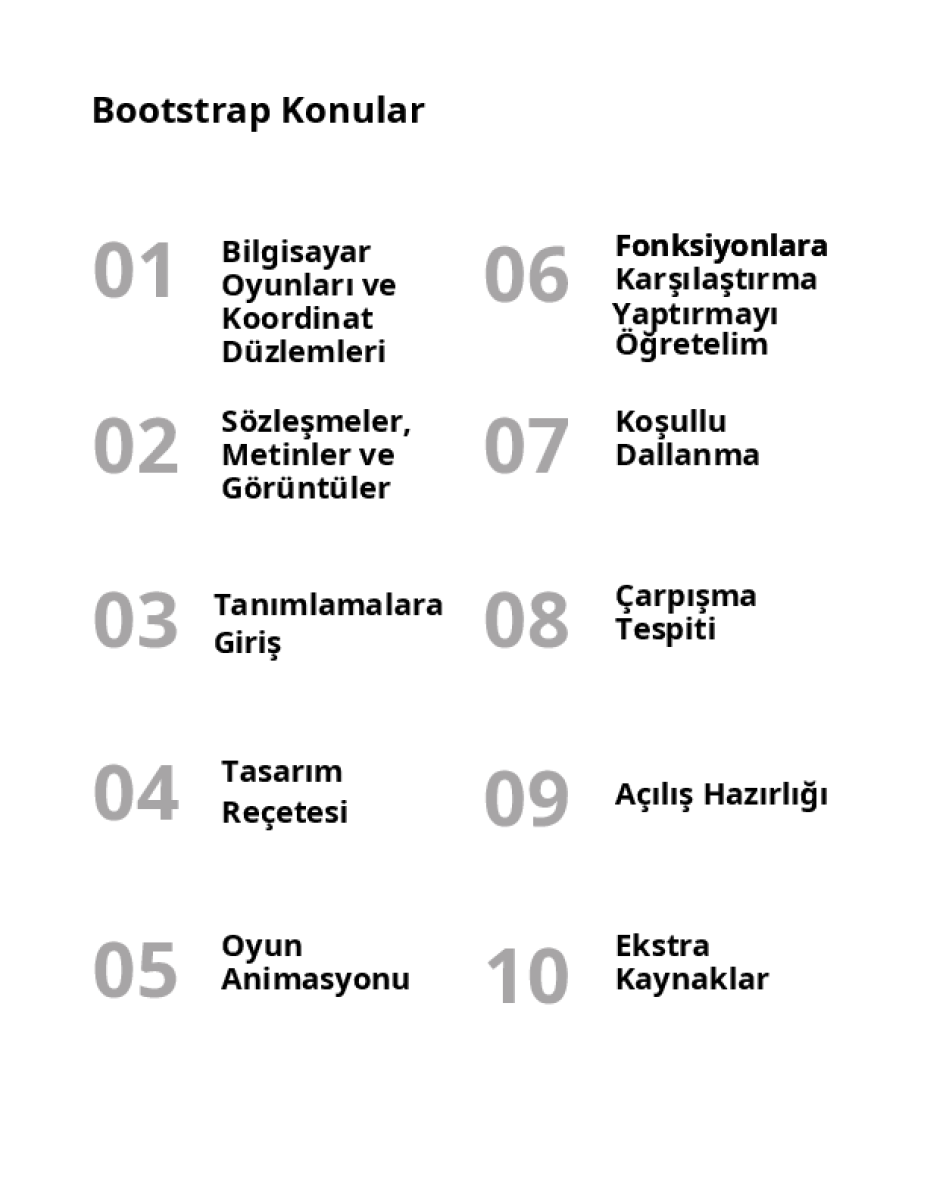
\includegraphics[width=1\linewidth]{cebirkapak-1.png}

\newpage
\includegraphics[width=1\linewidth]{cebir-bölüm-1-001.png}
\newpage
\includegraphics[width=1\linewidth]{cebirsplit-1.png}
\newpage
\includegraphics[width=1\linewidth]{cebirsplit-2.png}
\newpage
\includegraphics[width=1\linewidth]{cebirsplit-3.png}
\newpage
\includegraphics[width=1\linewidth]{cebirsplit-4.png}
\newpage
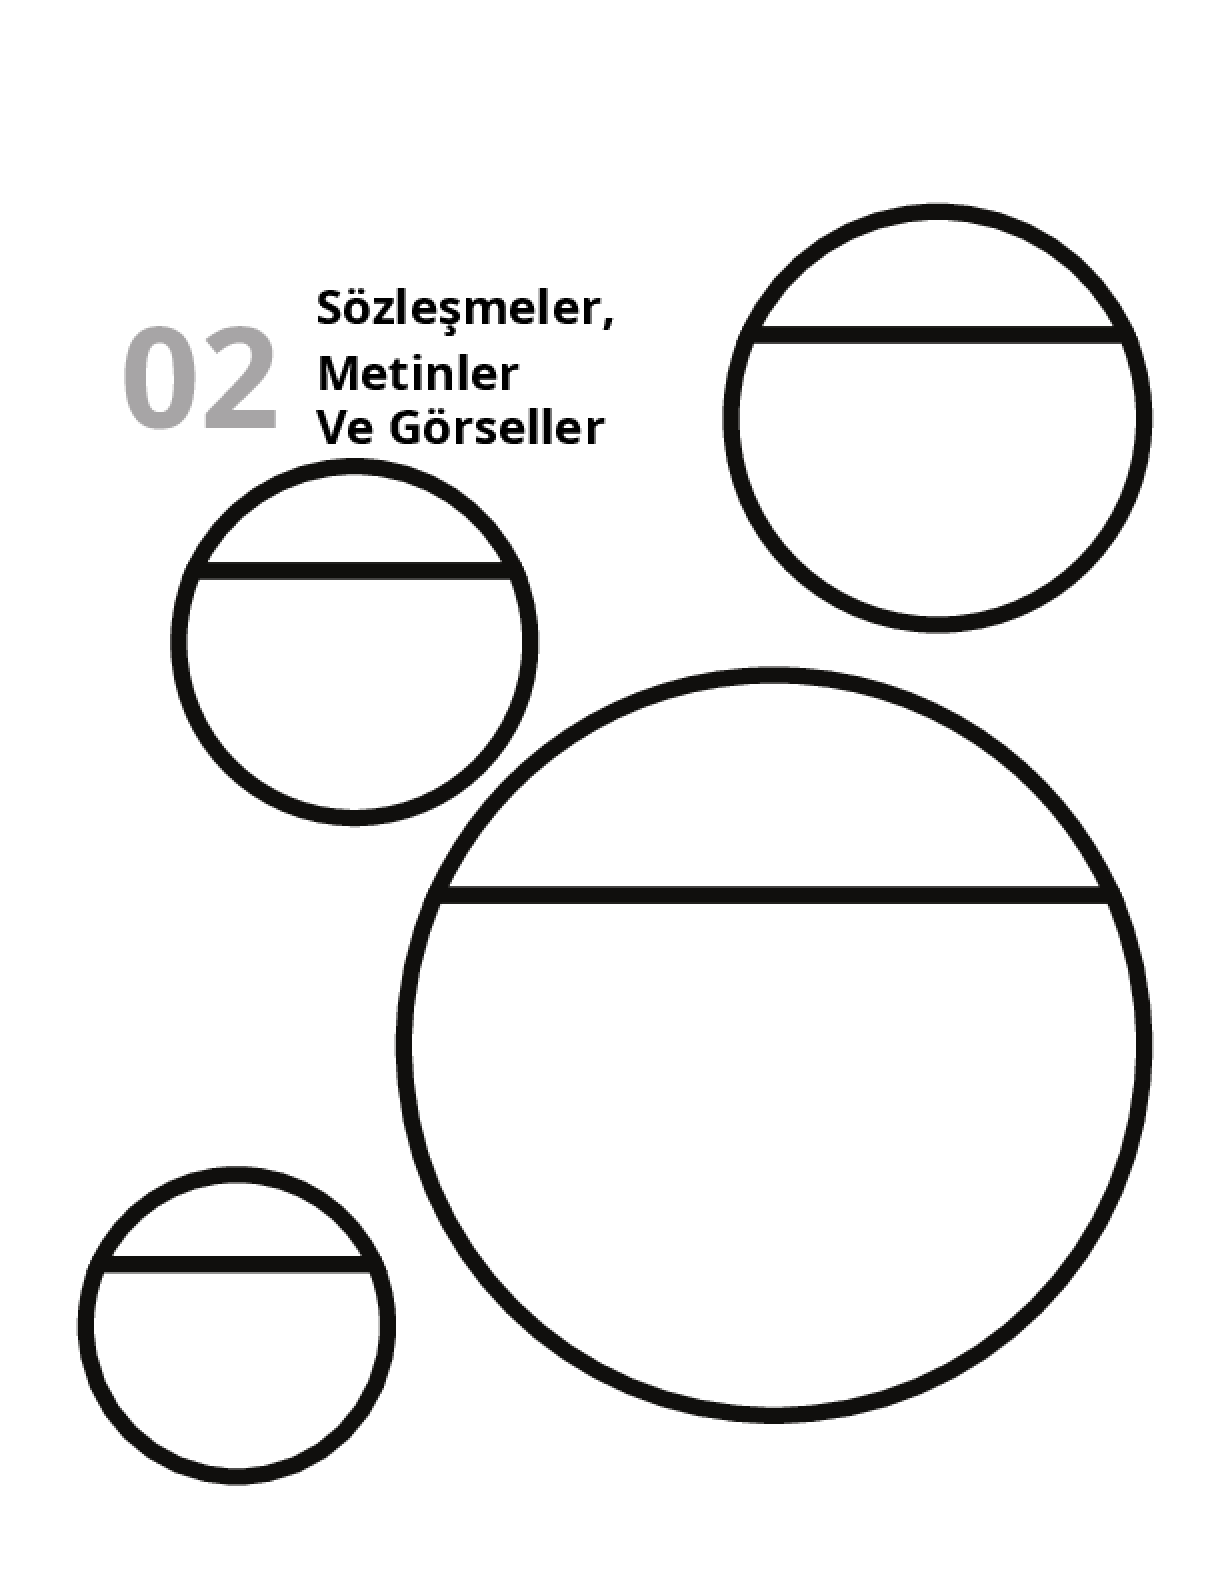
\includegraphics[width=1\linewidth]{cebirsplit-5.png}
\newpage
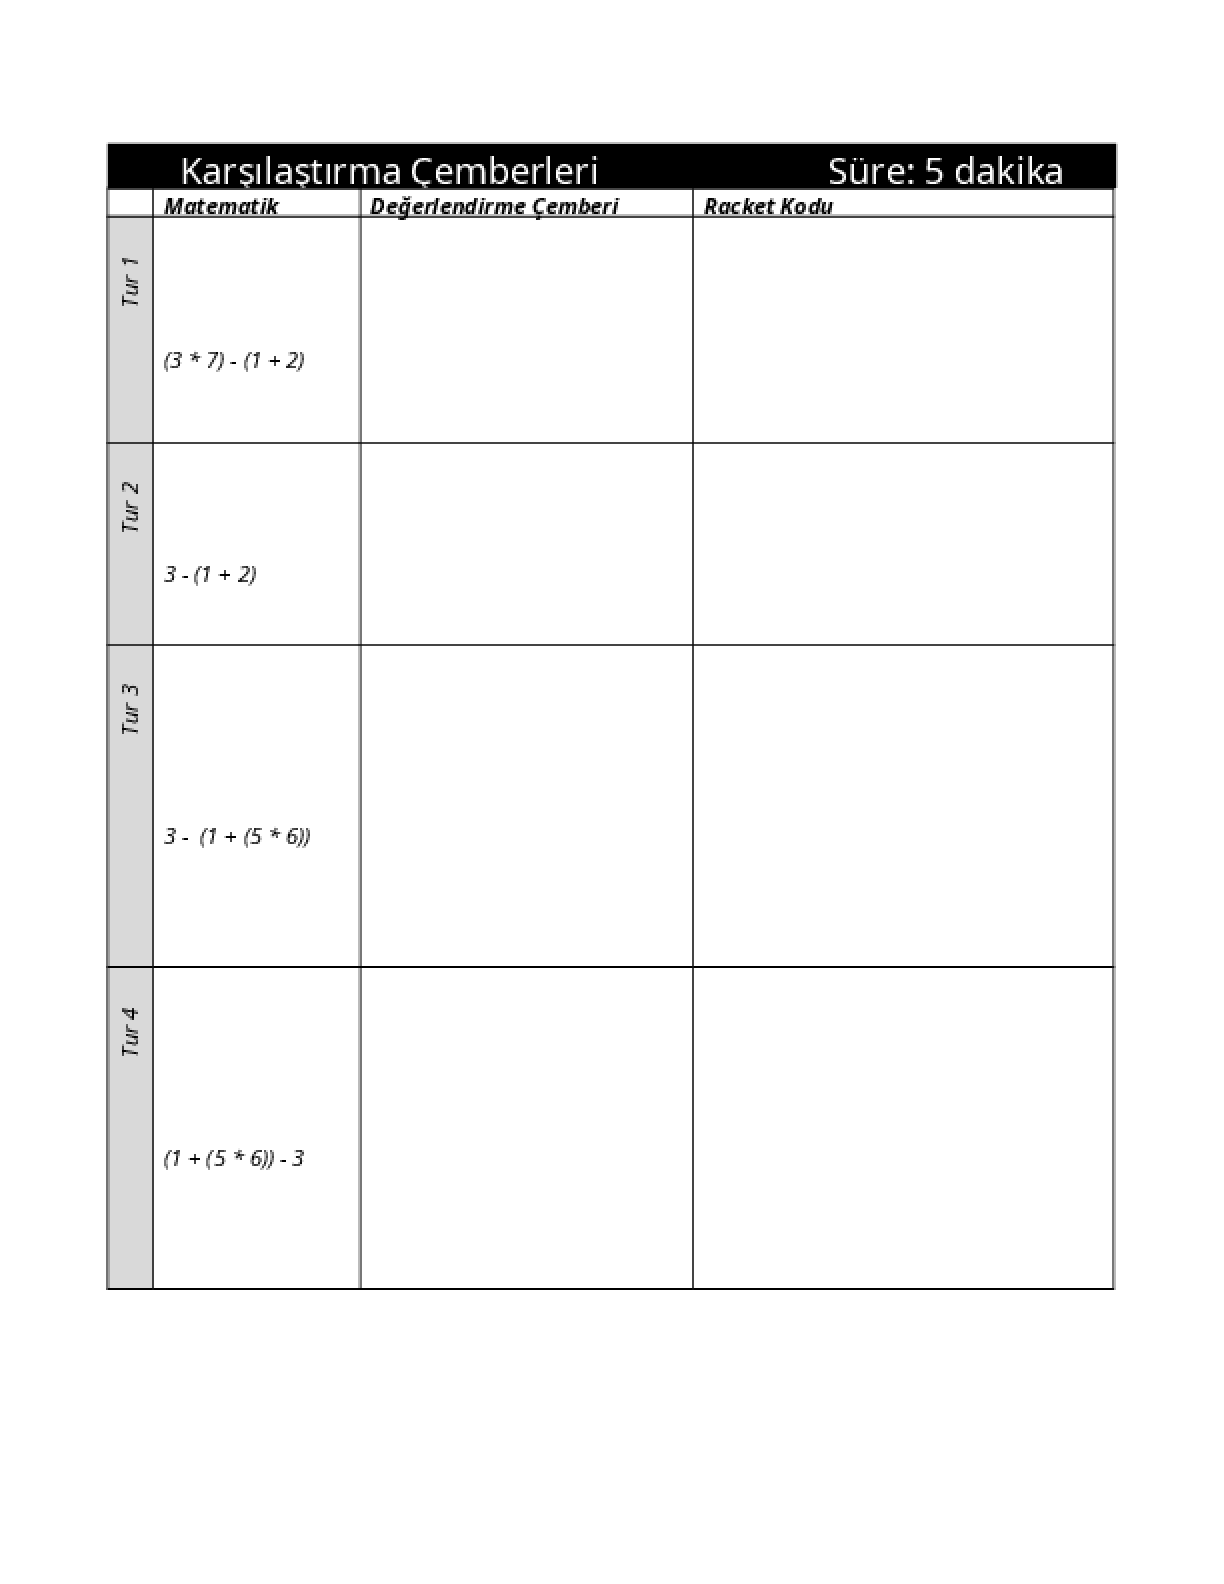
\includegraphics[width=1\linewidth]{cebirsplit-6.png}
\newpage
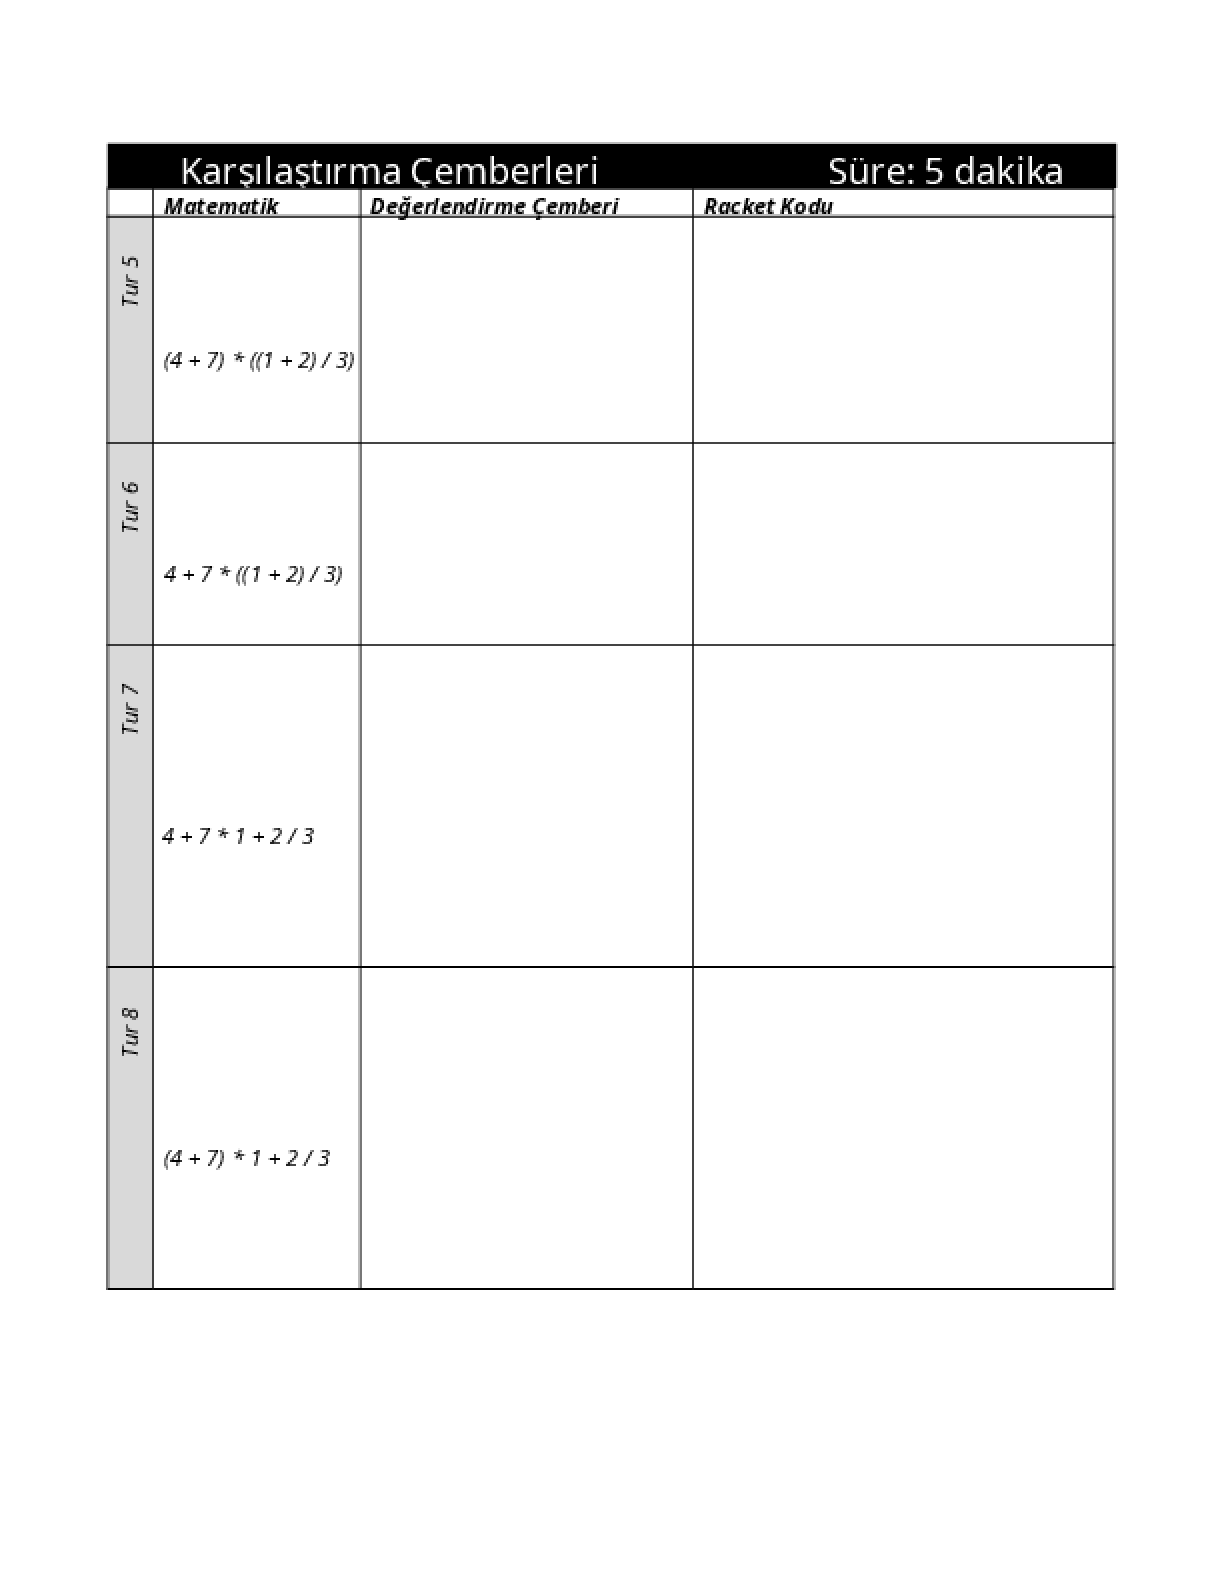
\includegraphics[width=1\linewidth]{cebirsplit-7.png}
\newpage
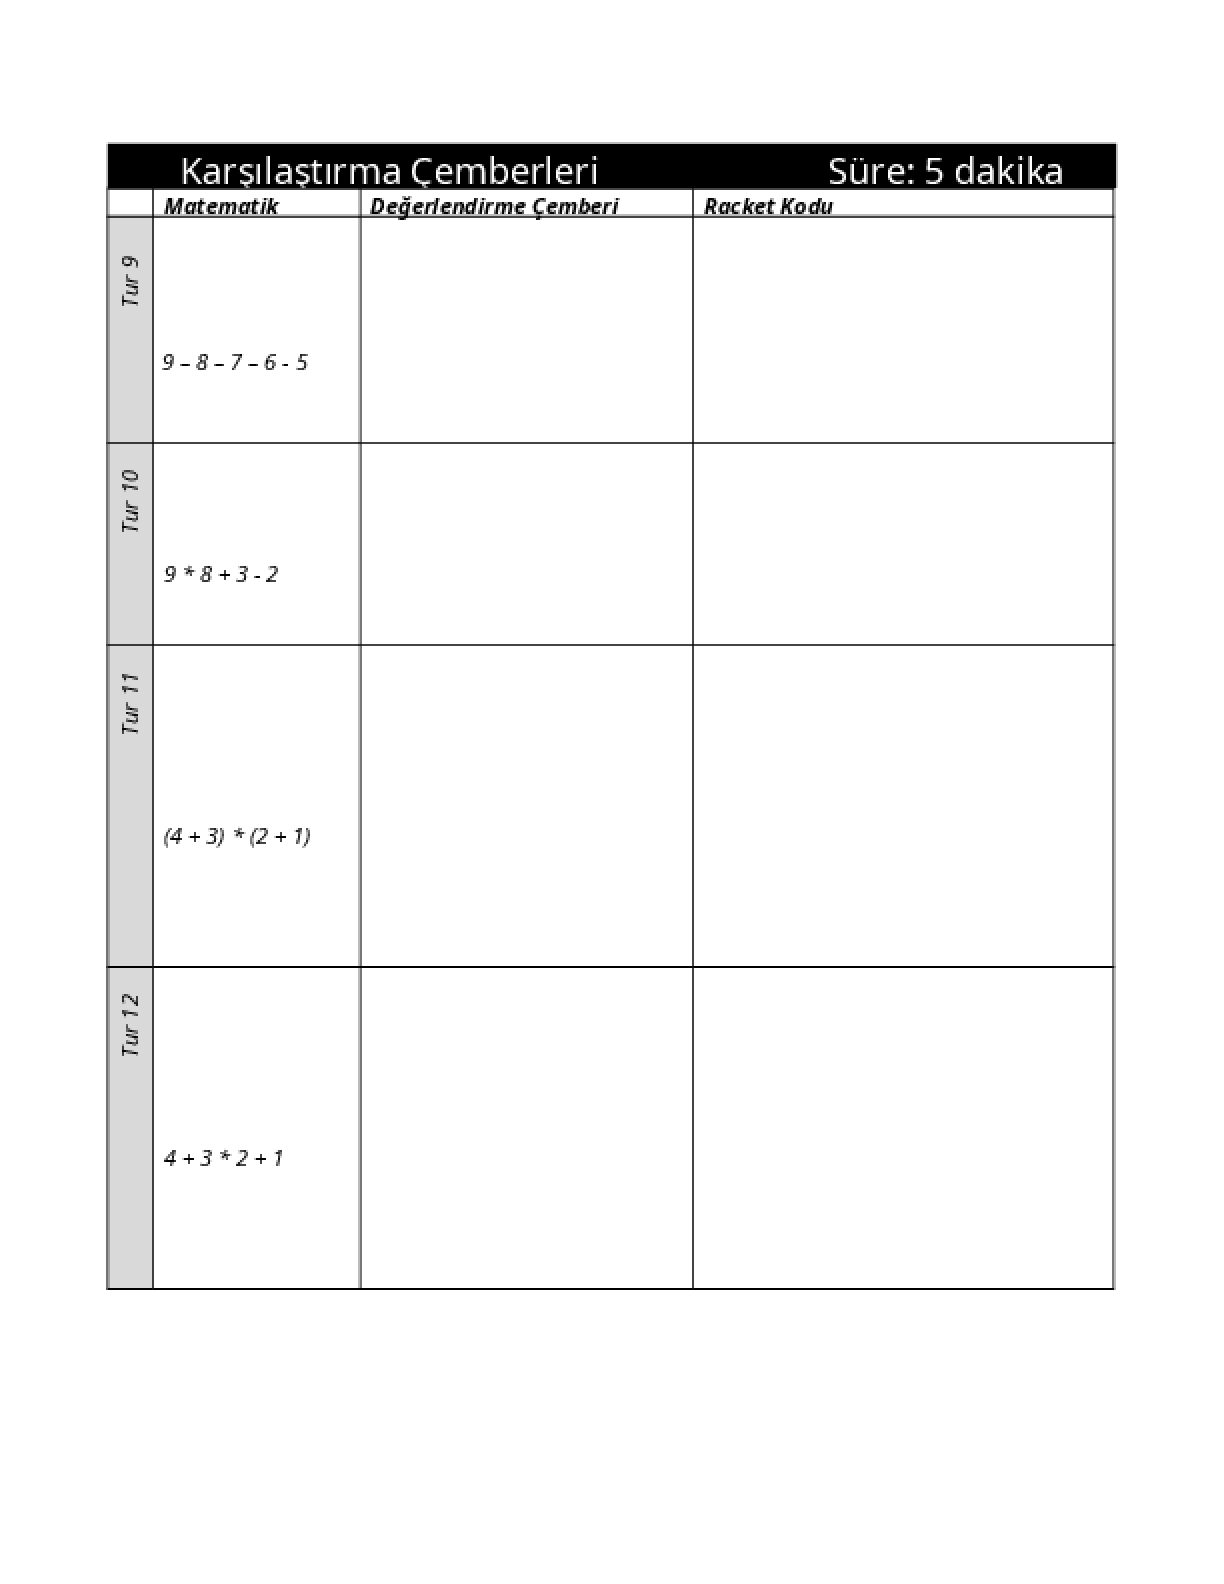
\includegraphics[width=1\linewidth]{cebirsplit-8.png}
\newpage
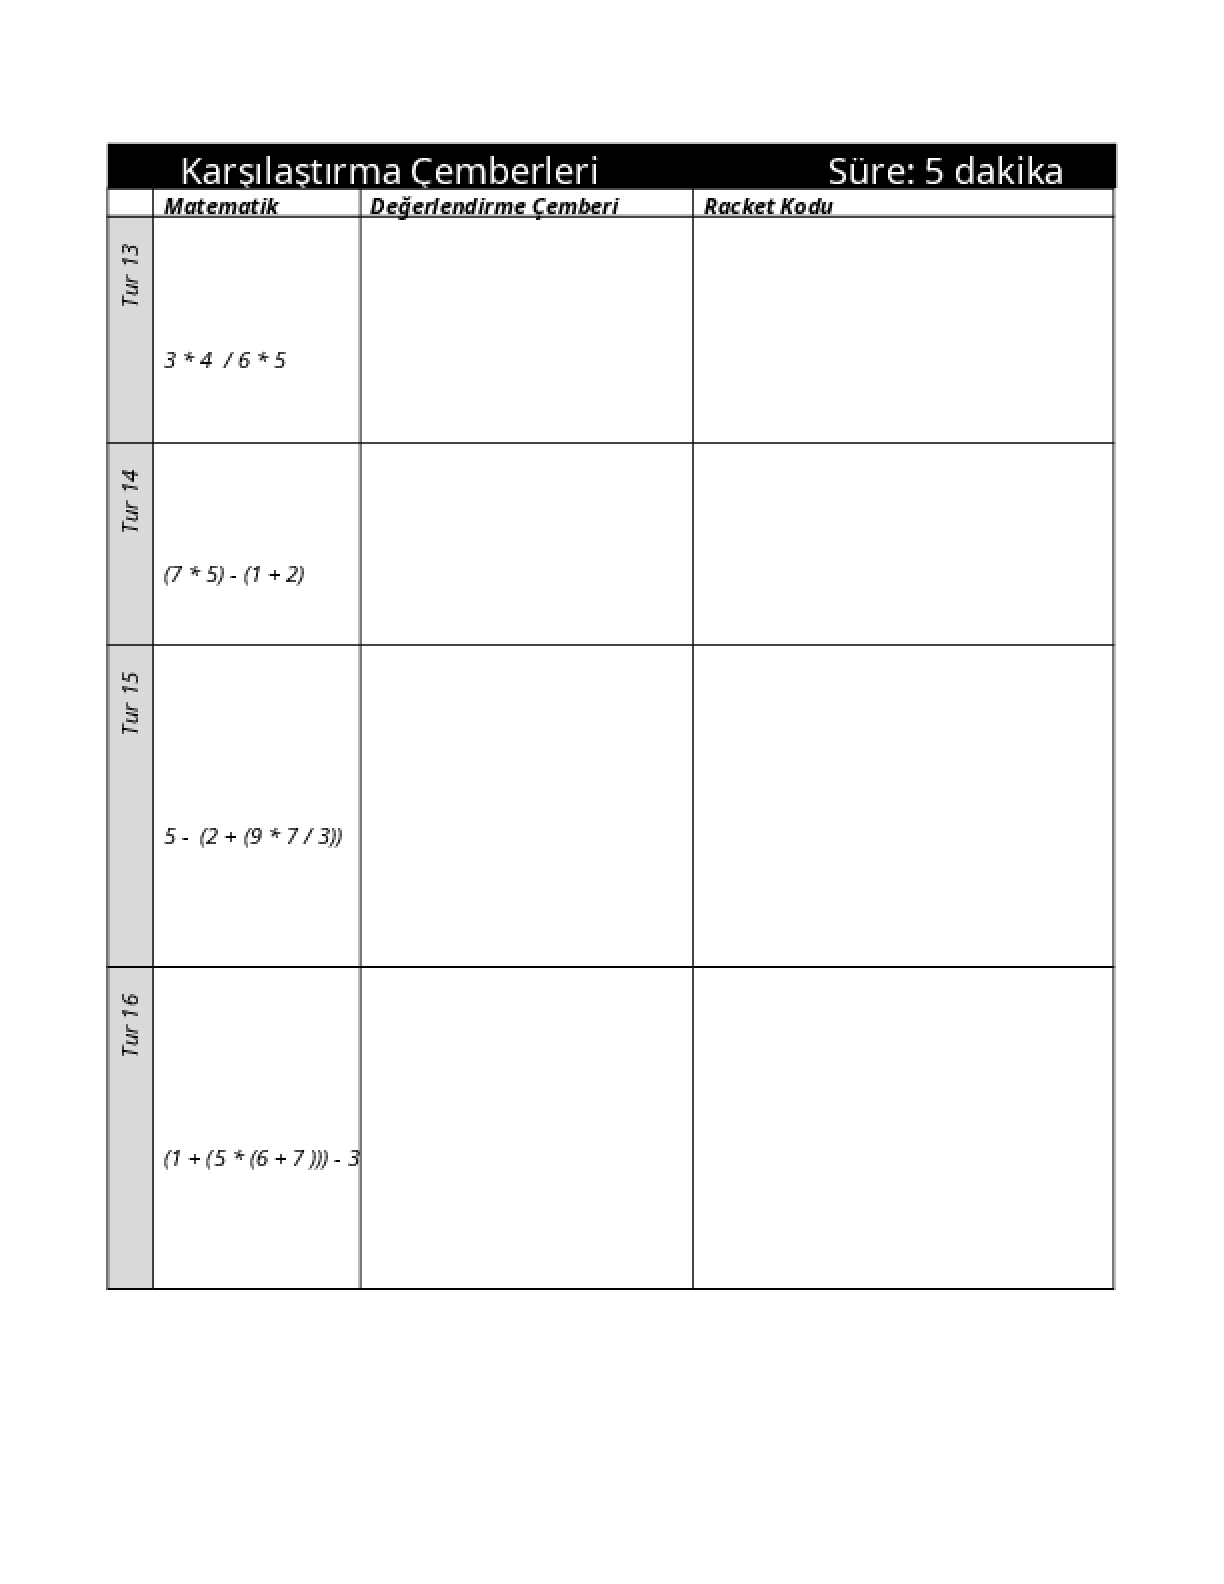
\includegraphics[width=1\linewidth]{cebirsplit-9.png}
\newpage
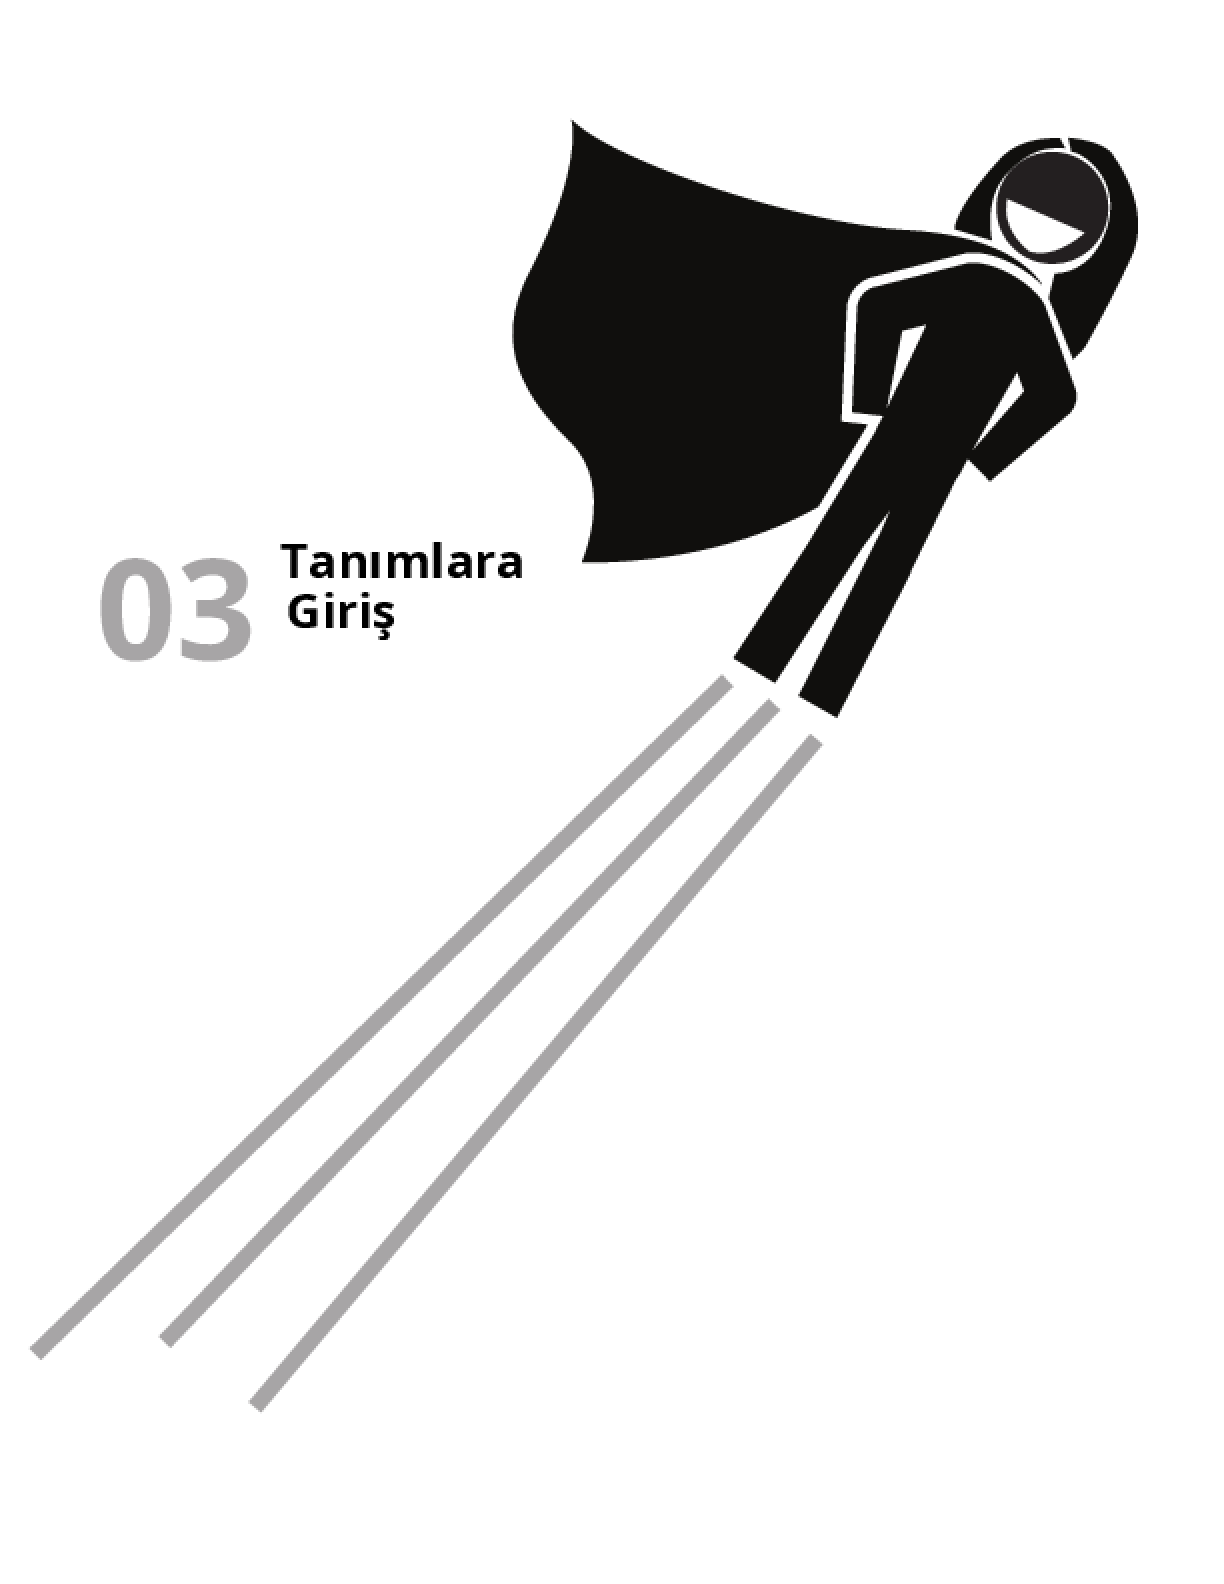
\includegraphics[width=1\linewidth]{cebirsplit-10.png}
\newpage
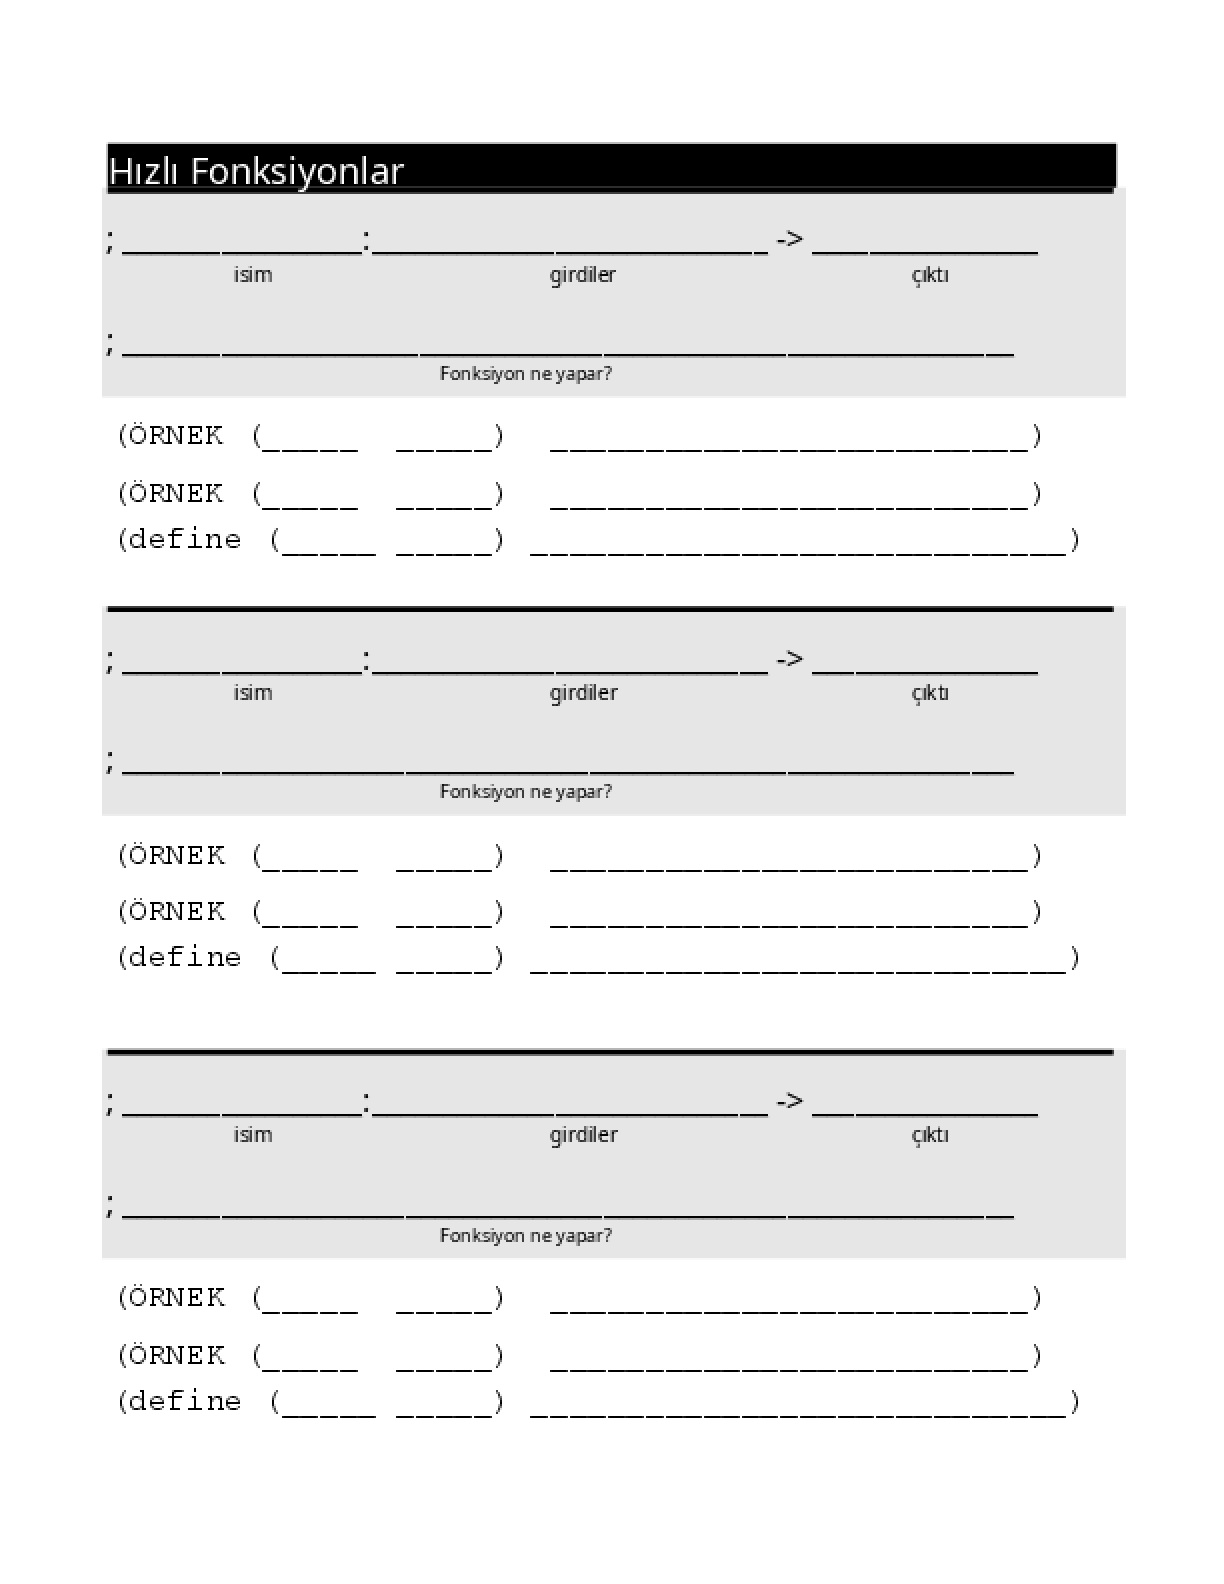
\includegraphics[width=1\linewidth]{cebirsplit-11.png}
\newpage
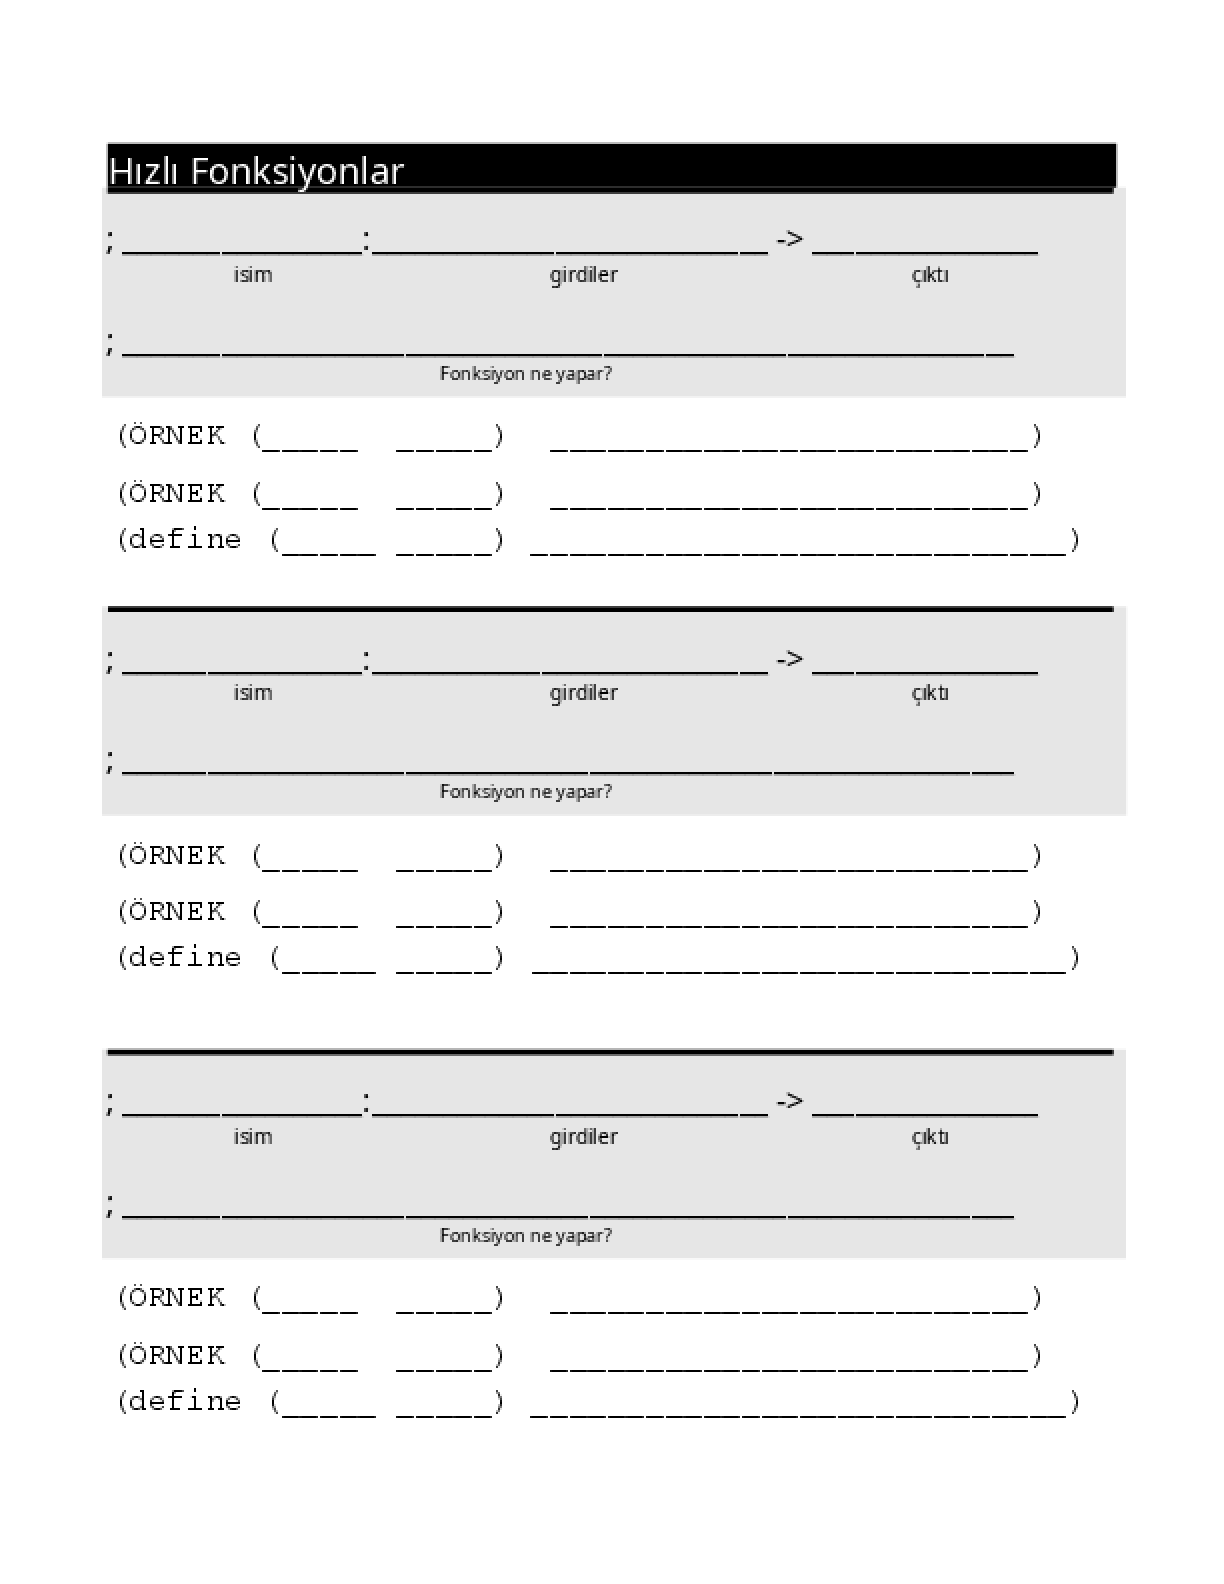
\includegraphics[width=1\linewidth]{cebirsplit-12.png}
\newpage
\includegraphics[width=1\linewidth]{cebirsplit-13.png}
\newpage
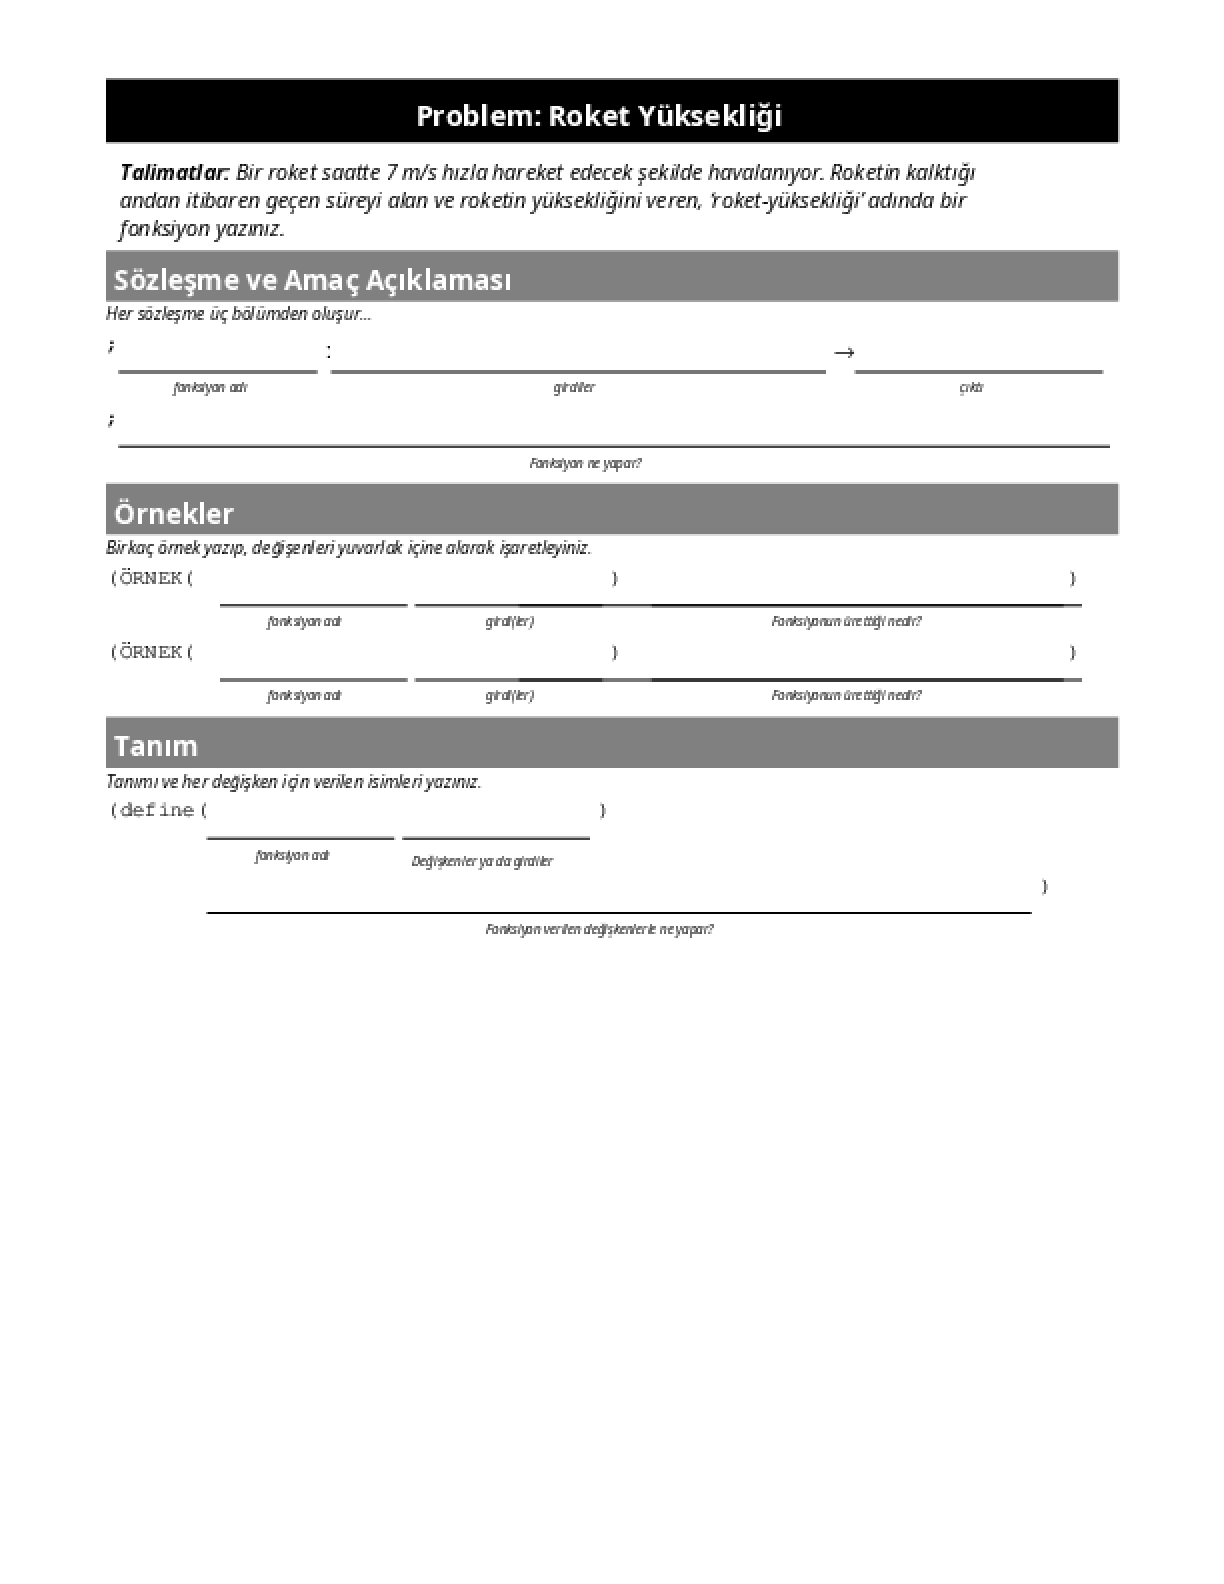
\includegraphics[width=1\linewidth]{cebirsplit-14.png}
\newpage
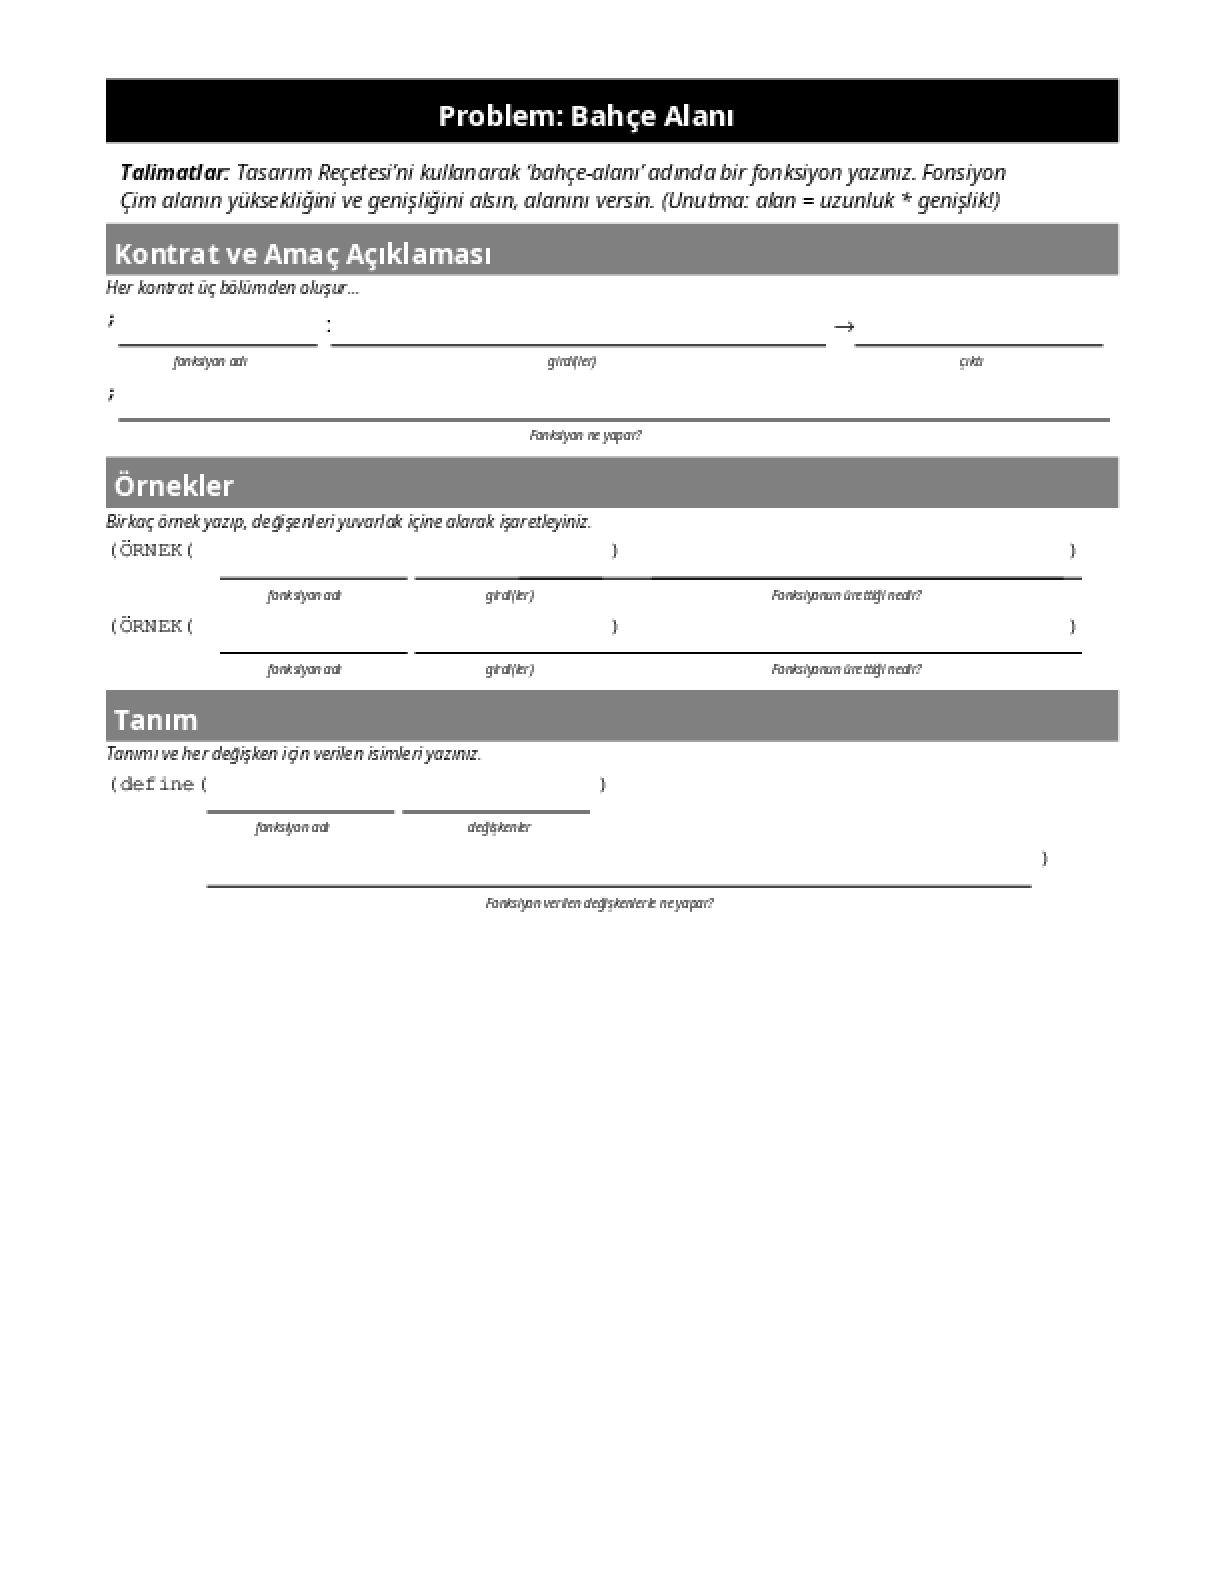
\includegraphics[width=1\linewidth]{cebirsplit-15.png}
\newpage
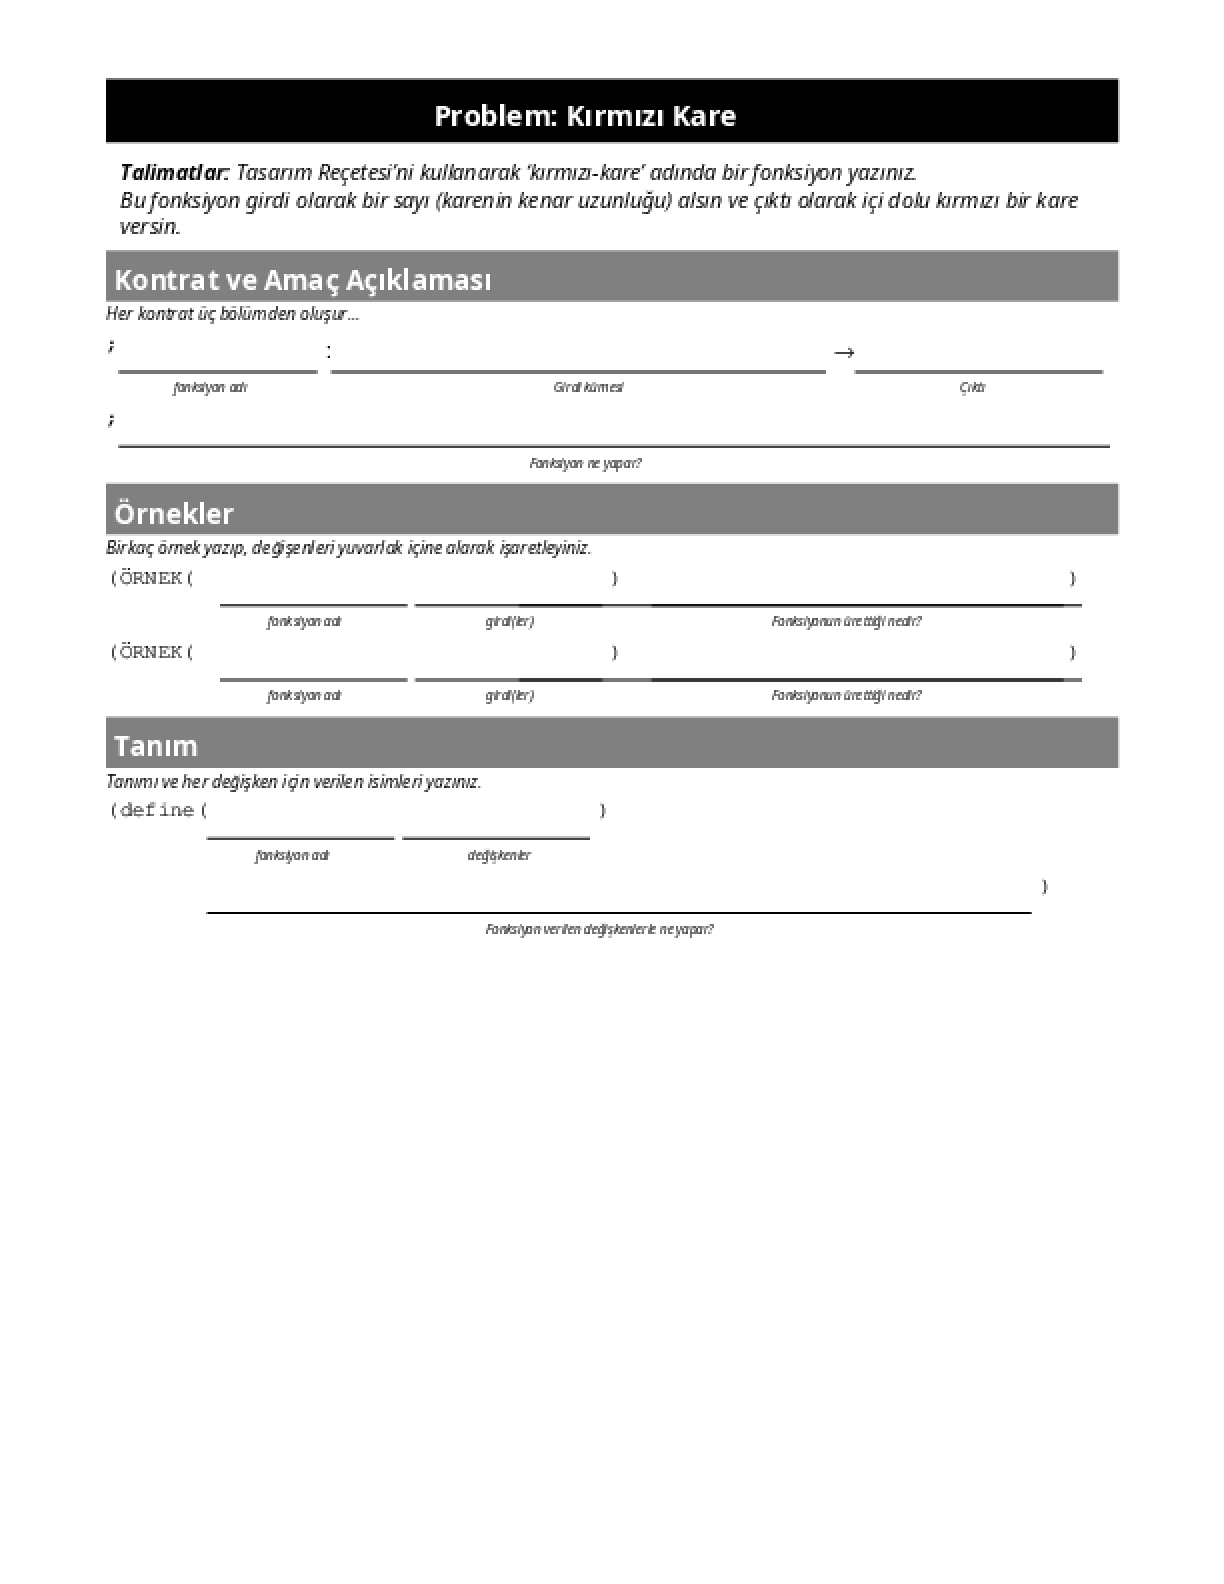
\includegraphics[width=1\linewidth]{cebirsplit-16.png}
\newpage
\includegraphics[width=1\linewidth]{cebirsplit-17.png}
\newpage
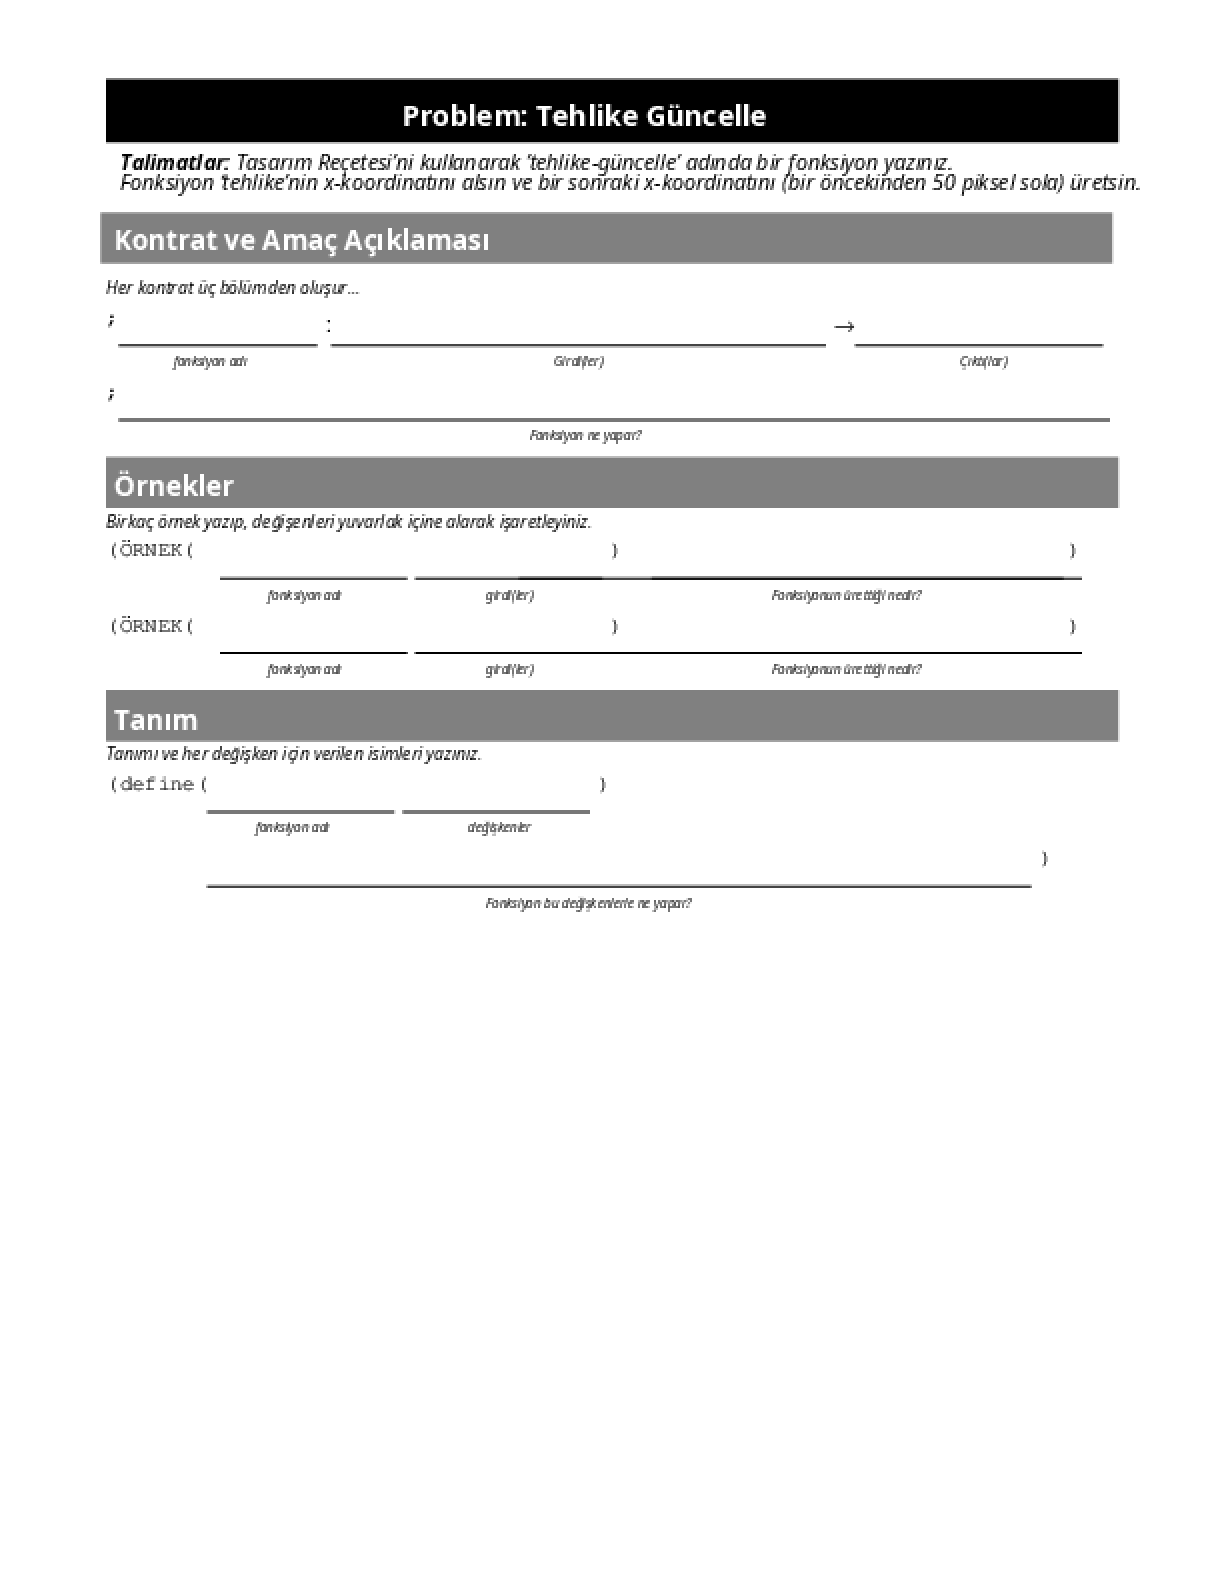
\includegraphics[width=1\linewidth]{cebirsplit-18.png}
\newpage
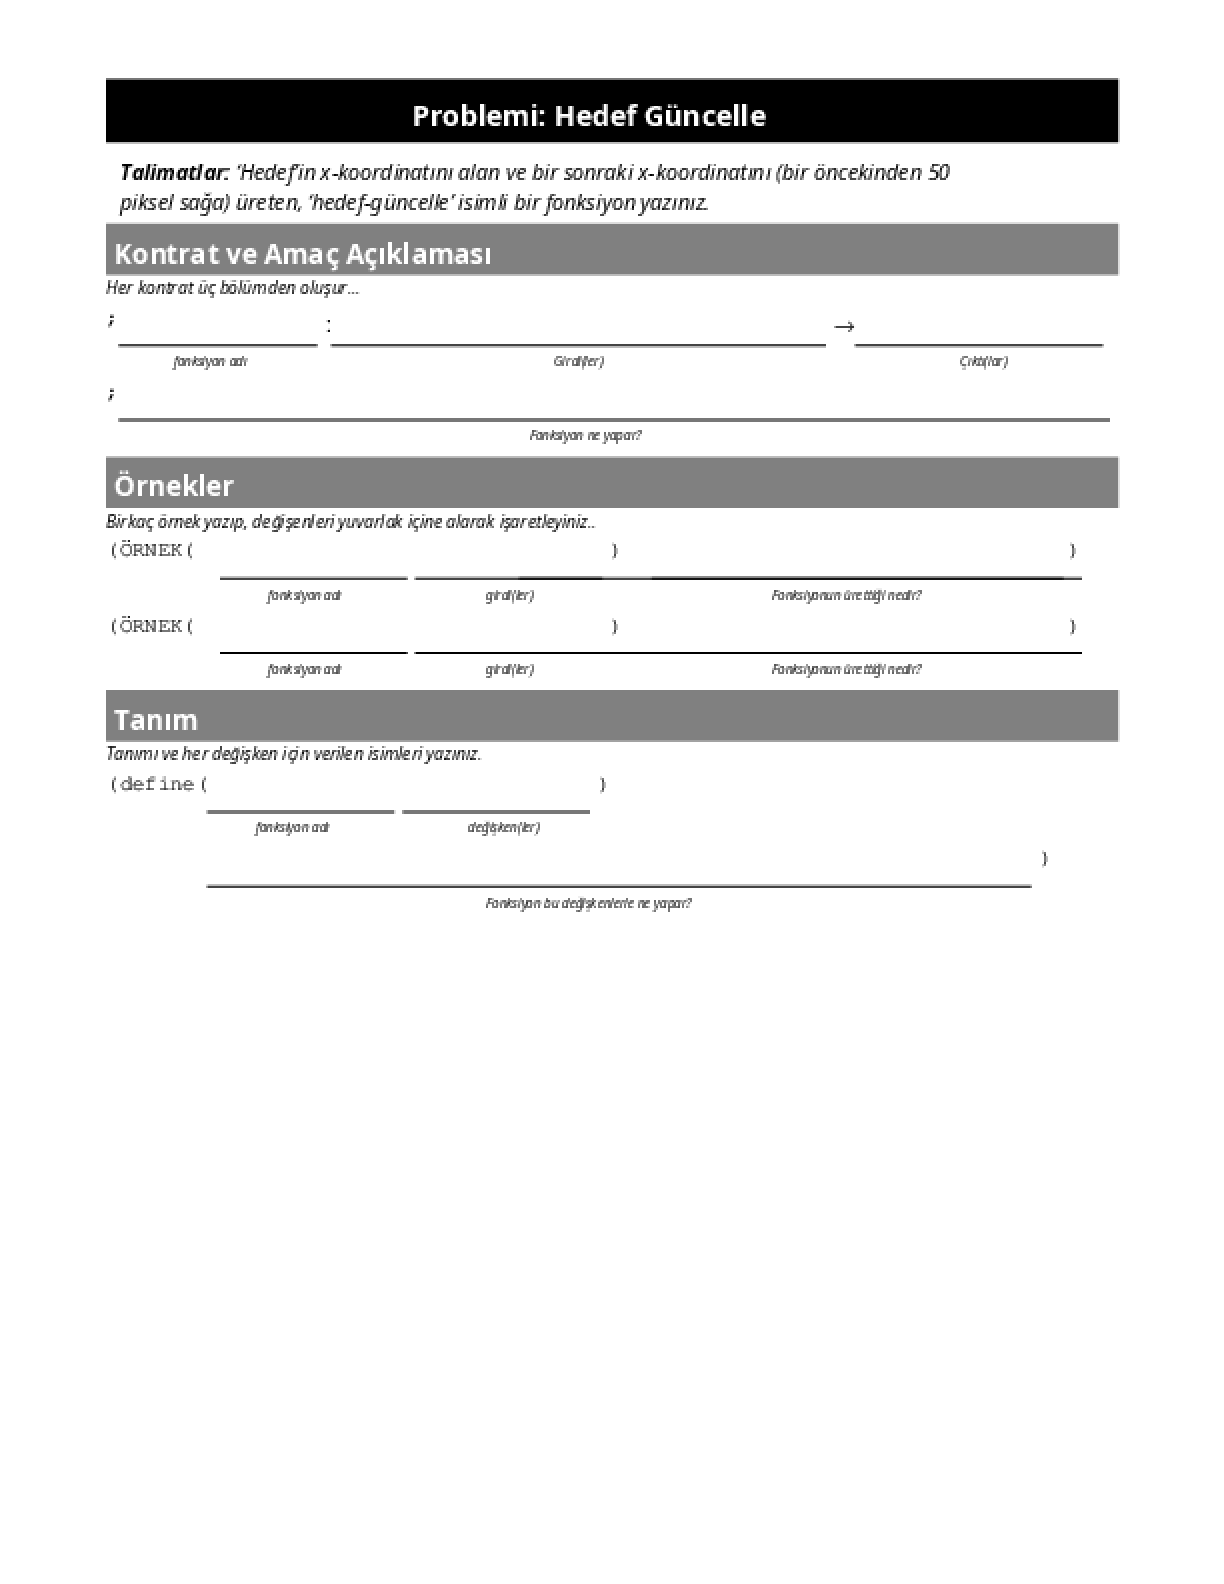
\includegraphics[width=1\linewidth]{cebirsplit-19.png}
\newpage
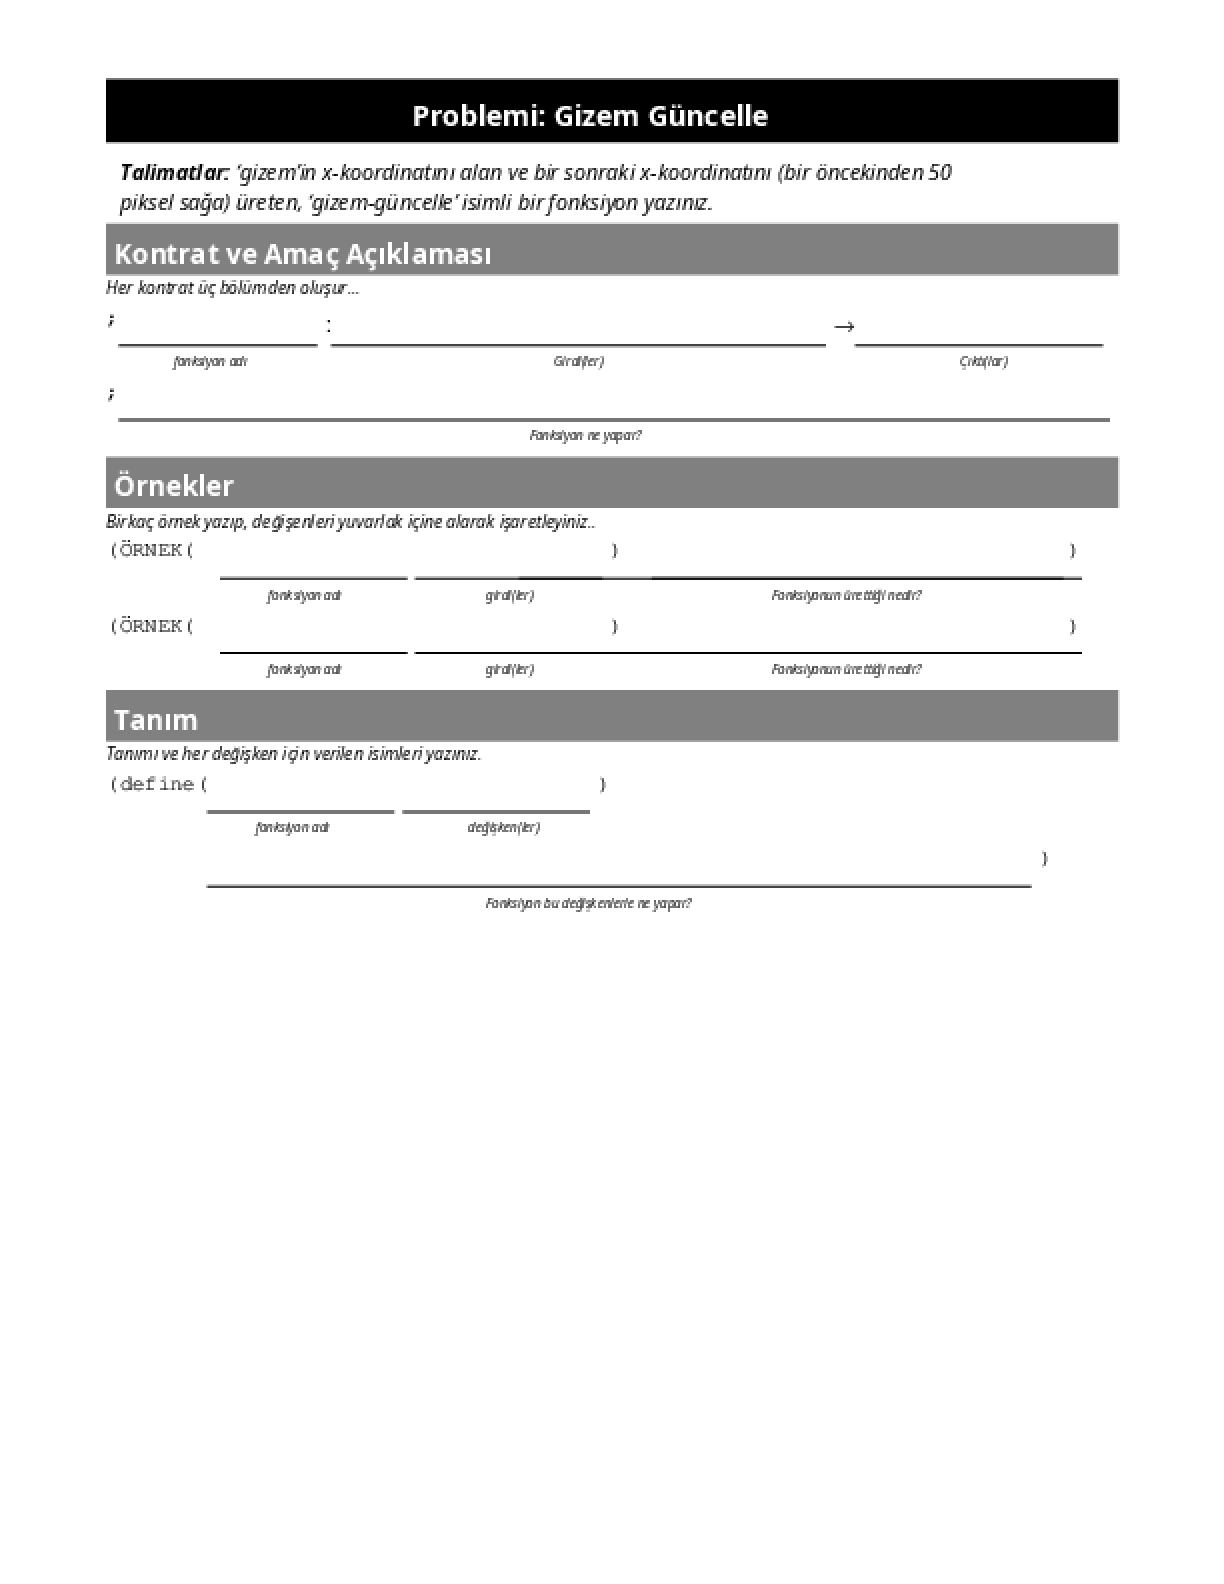
\includegraphics[width=1\linewidth]{cebirsplit-20.png}
\newpage
\includegraphics[width=1\linewidth]{cebirsplit-21.png}
\newpage
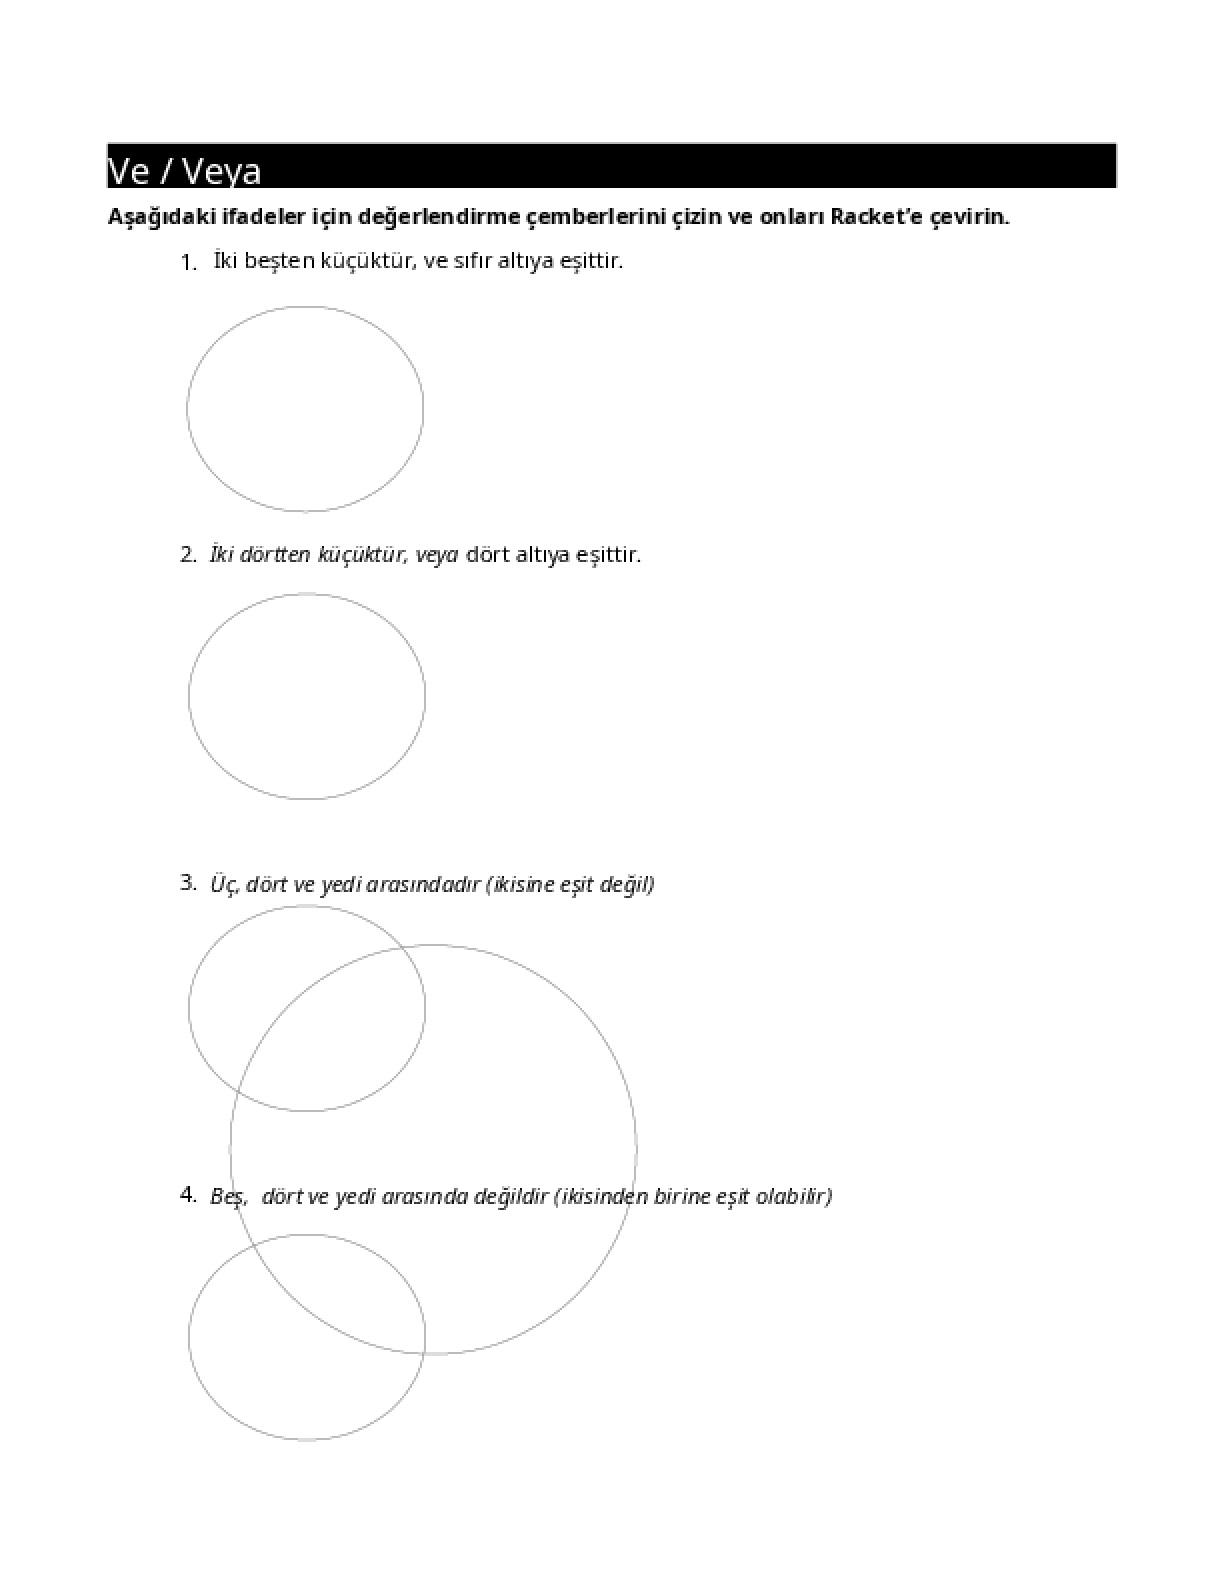
\includegraphics[width=1\linewidth]{cebirsplit-22.png}
\newpage
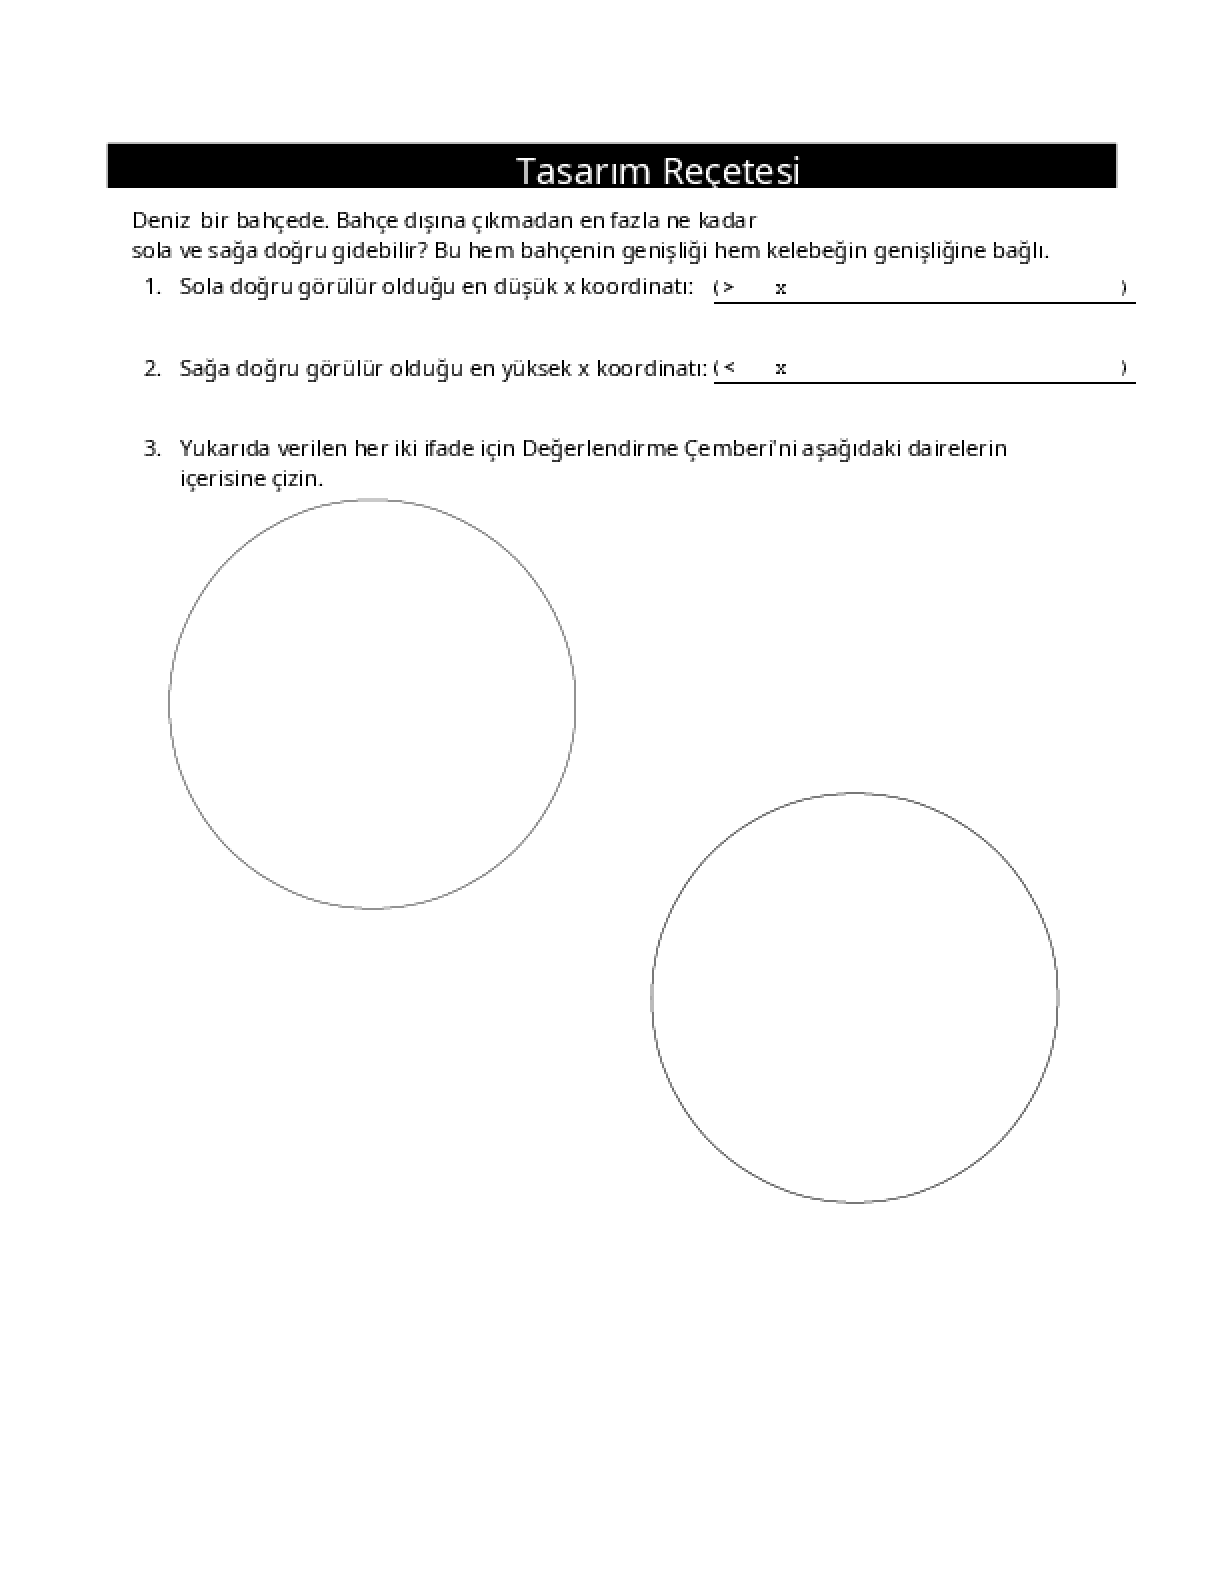
\includegraphics[width=1\linewidth]{cebirsplit-23.png}
\newpage
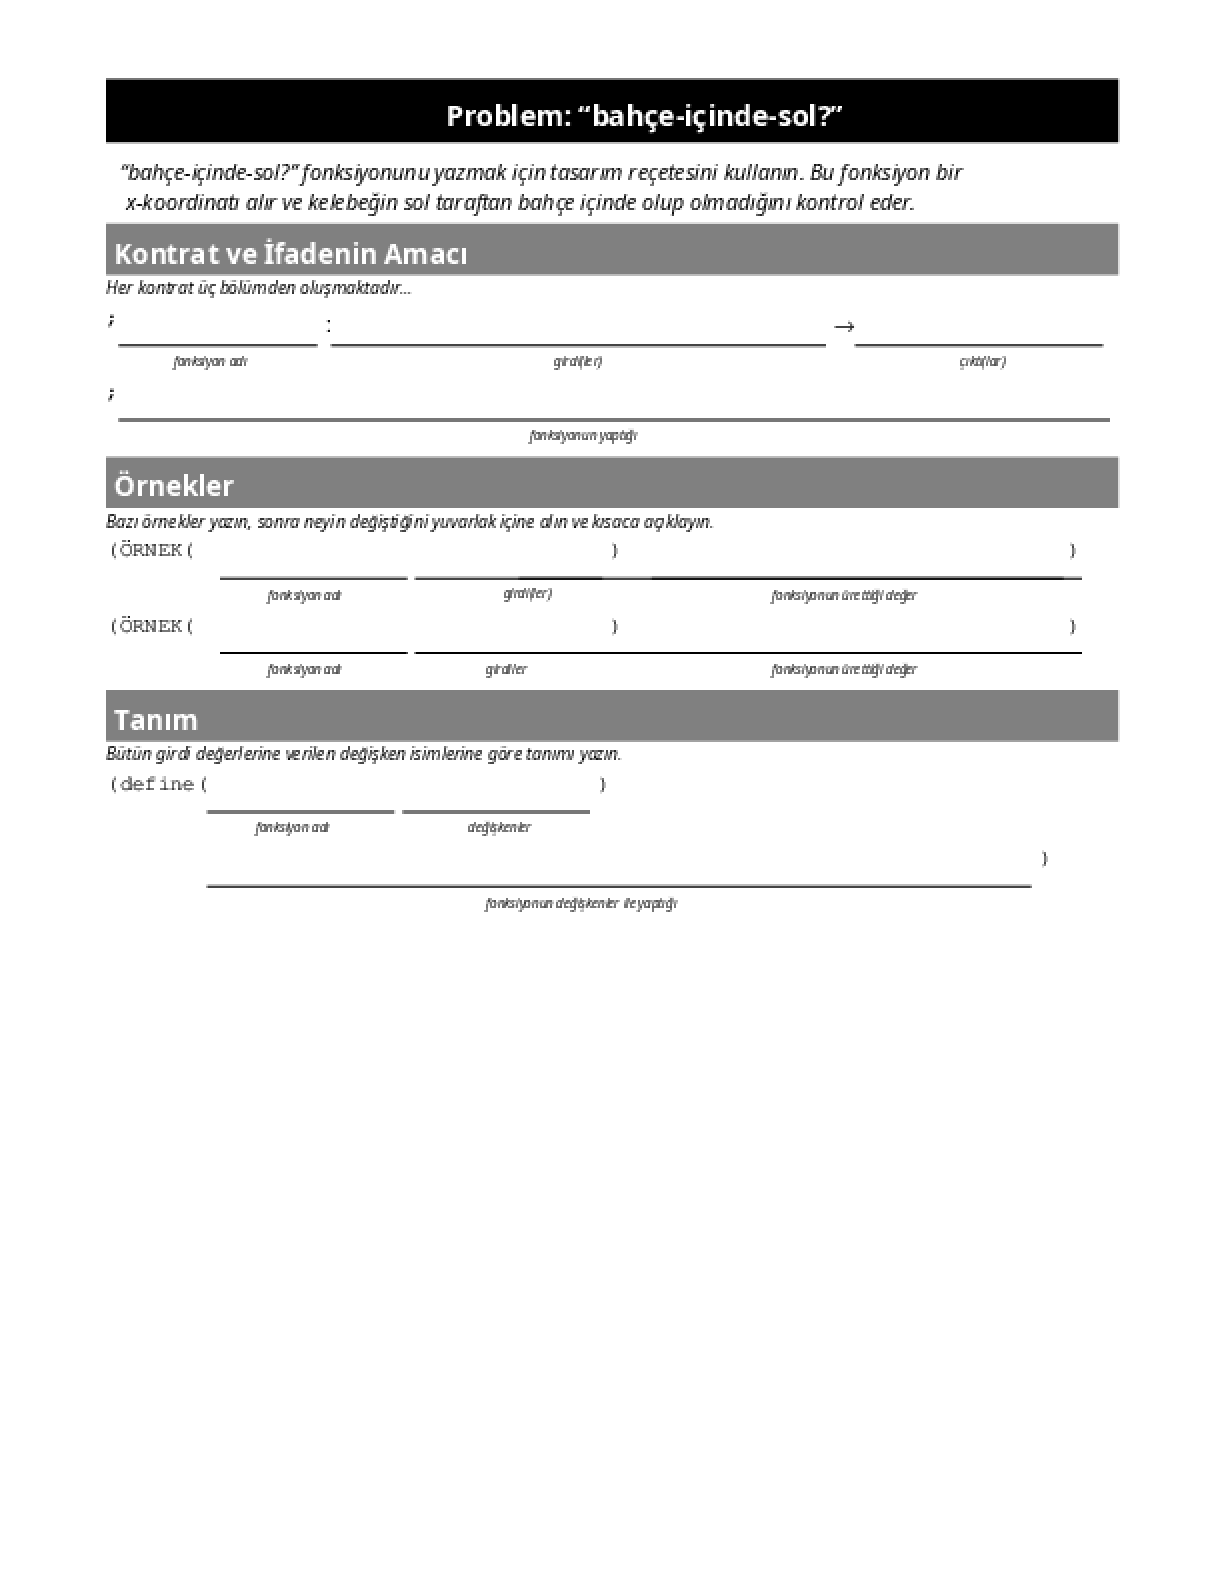
\includegraphics[width=1\linewidth]{cebirsplit-24.png}
\newpage
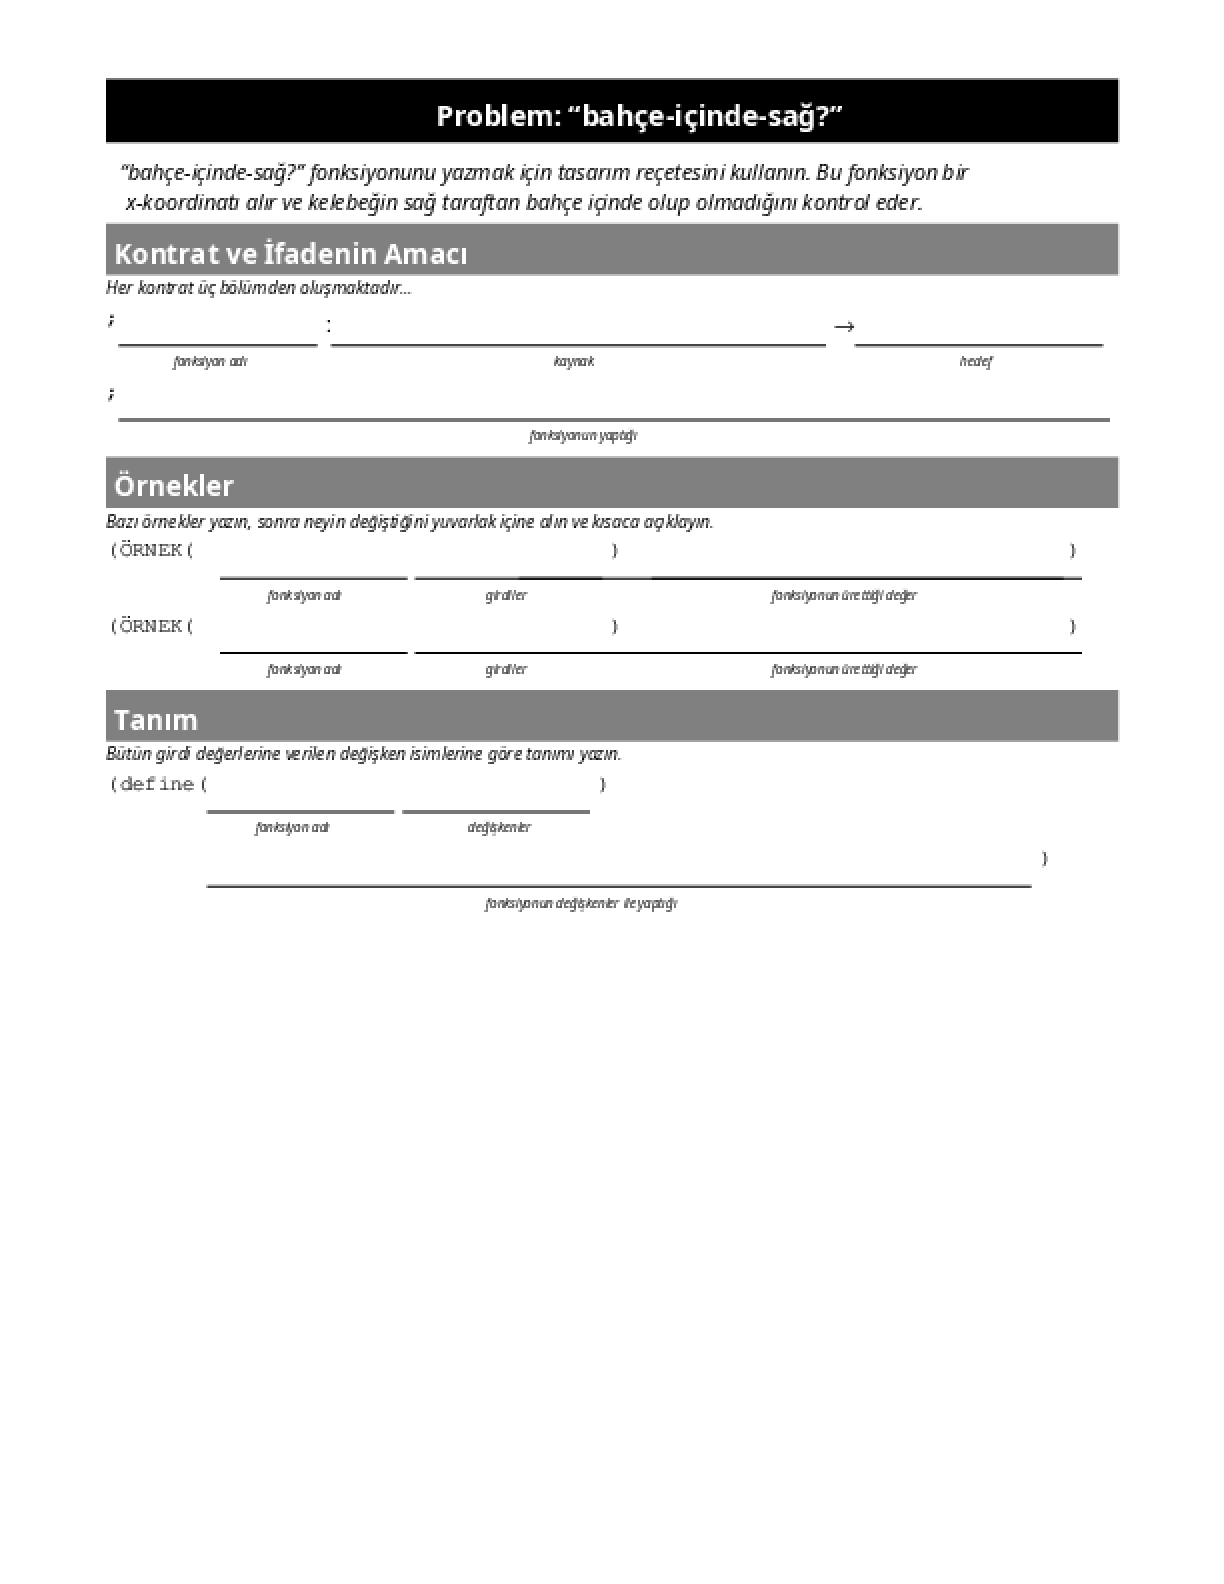
\includegraphics[width=1\linewidth]{cebirsplit-25.png}
\newpage
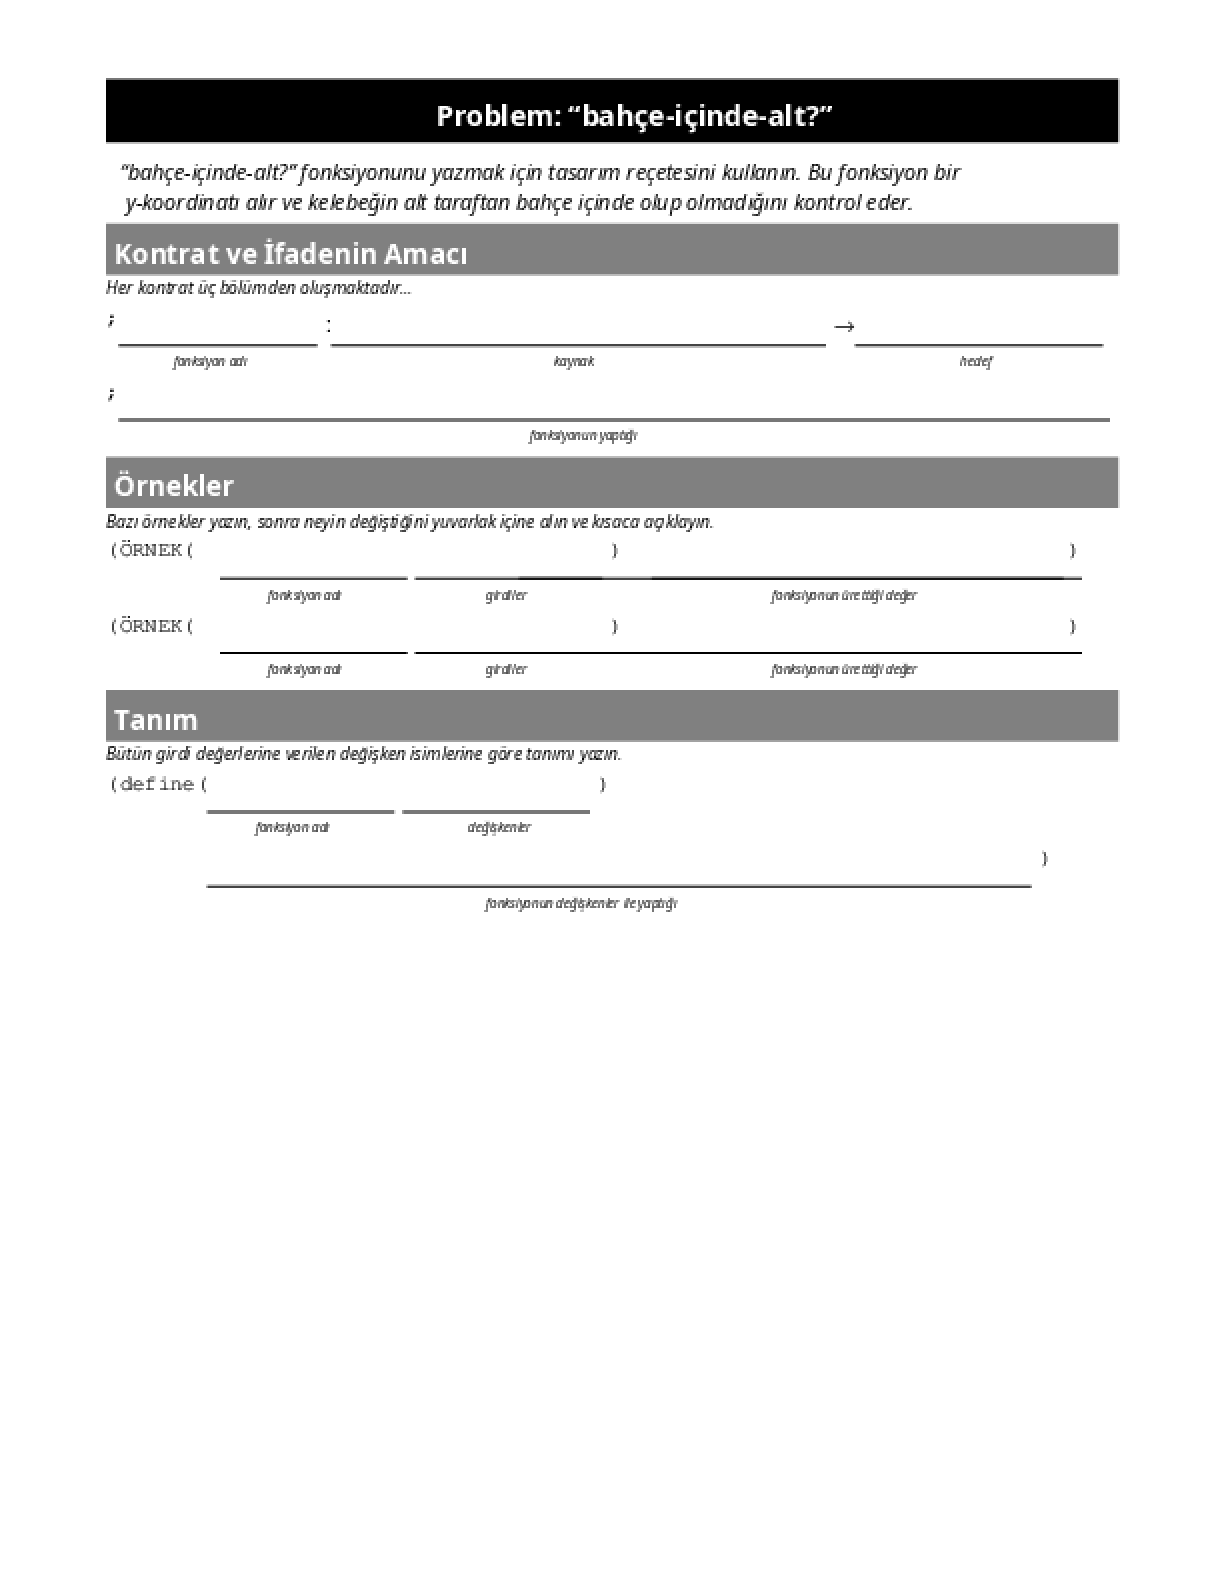
\includegraphics[width=1\linewidth]{cebirsplit-26.png}
\newpage
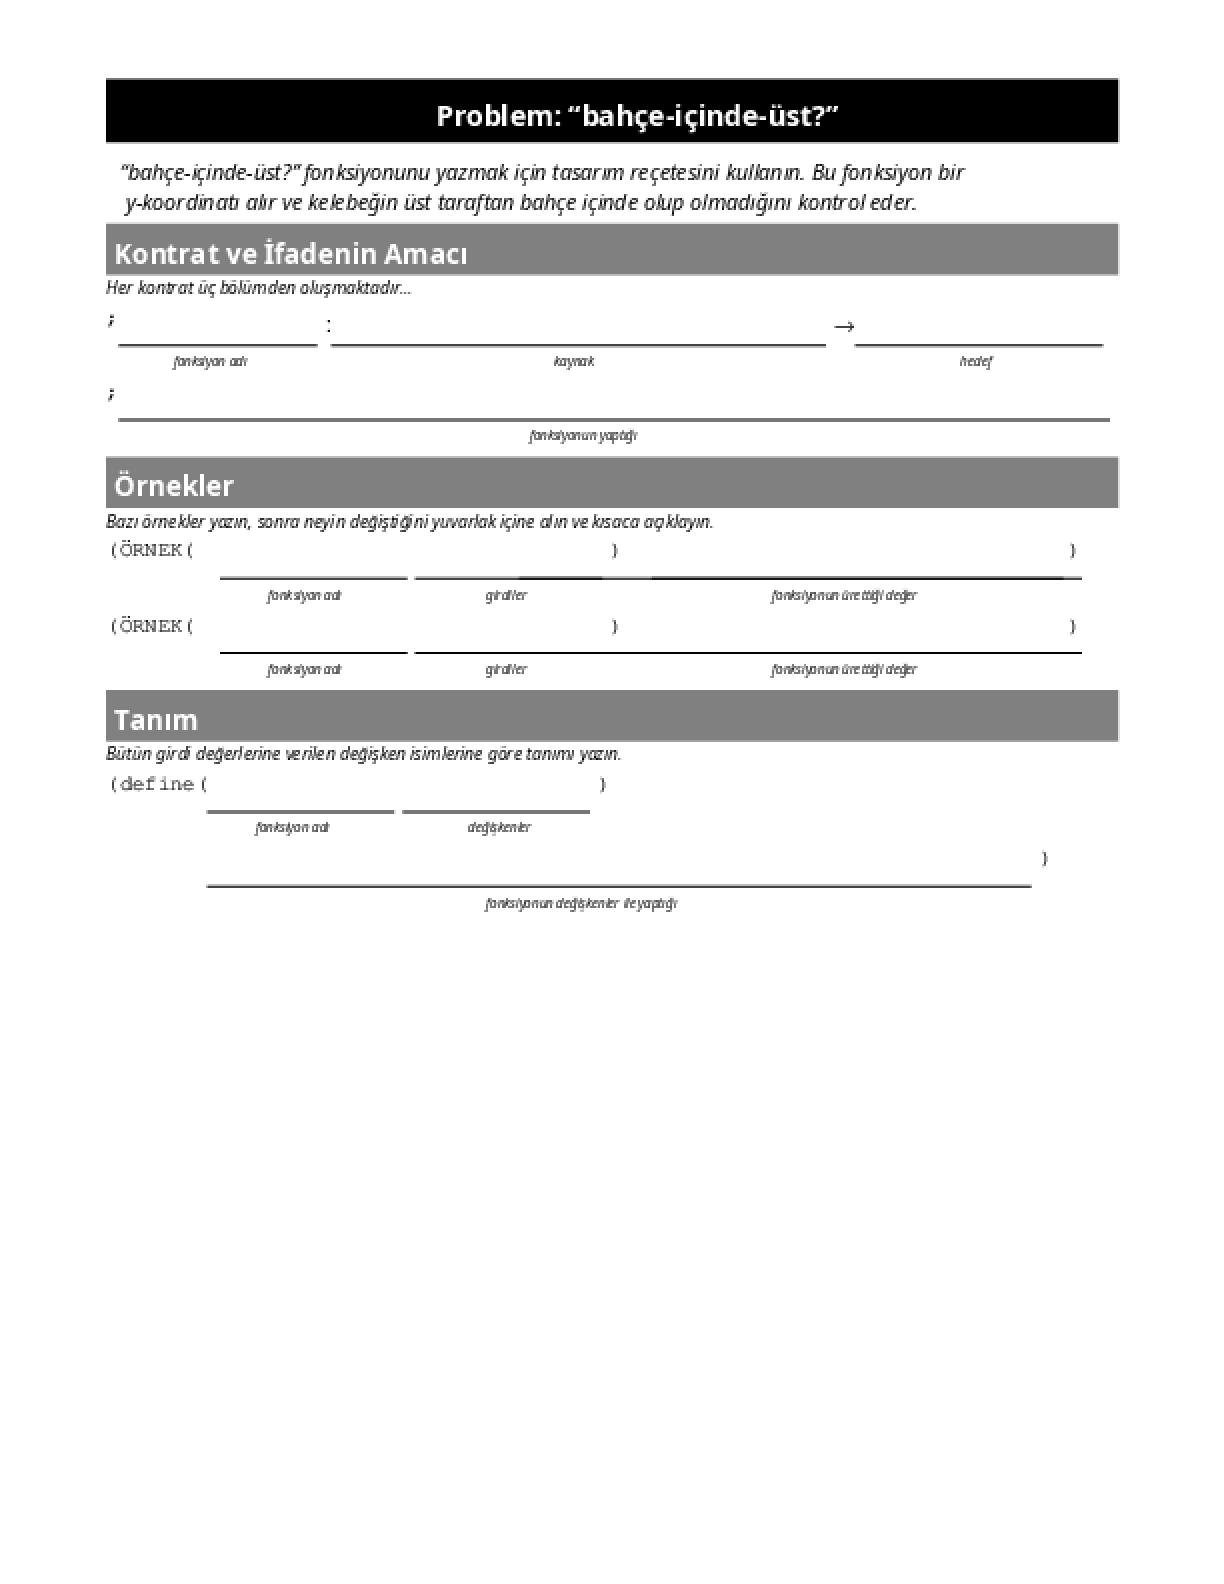
\includegraphics[width=1\linewidth]{cebirsplit-27.png}
\newpage
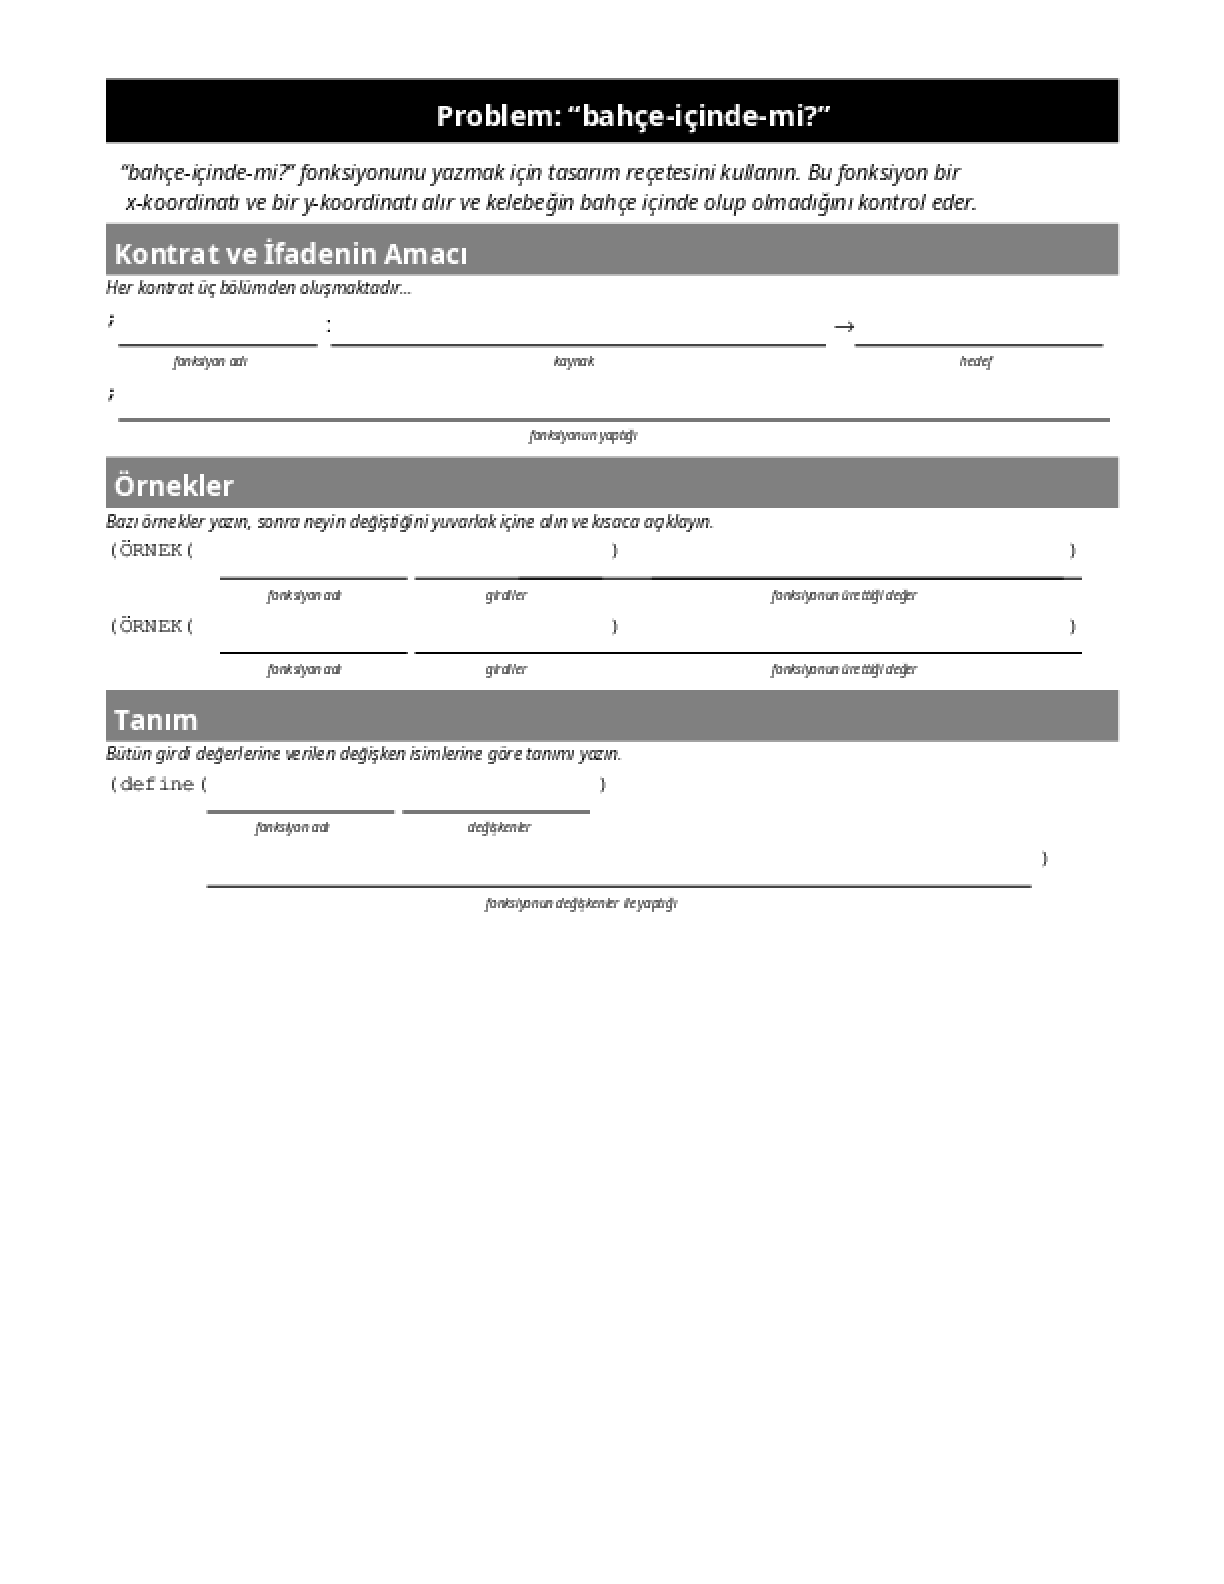
\includegraphics[width=1\linewidth]{cebirsplit-28.png}
\newpage
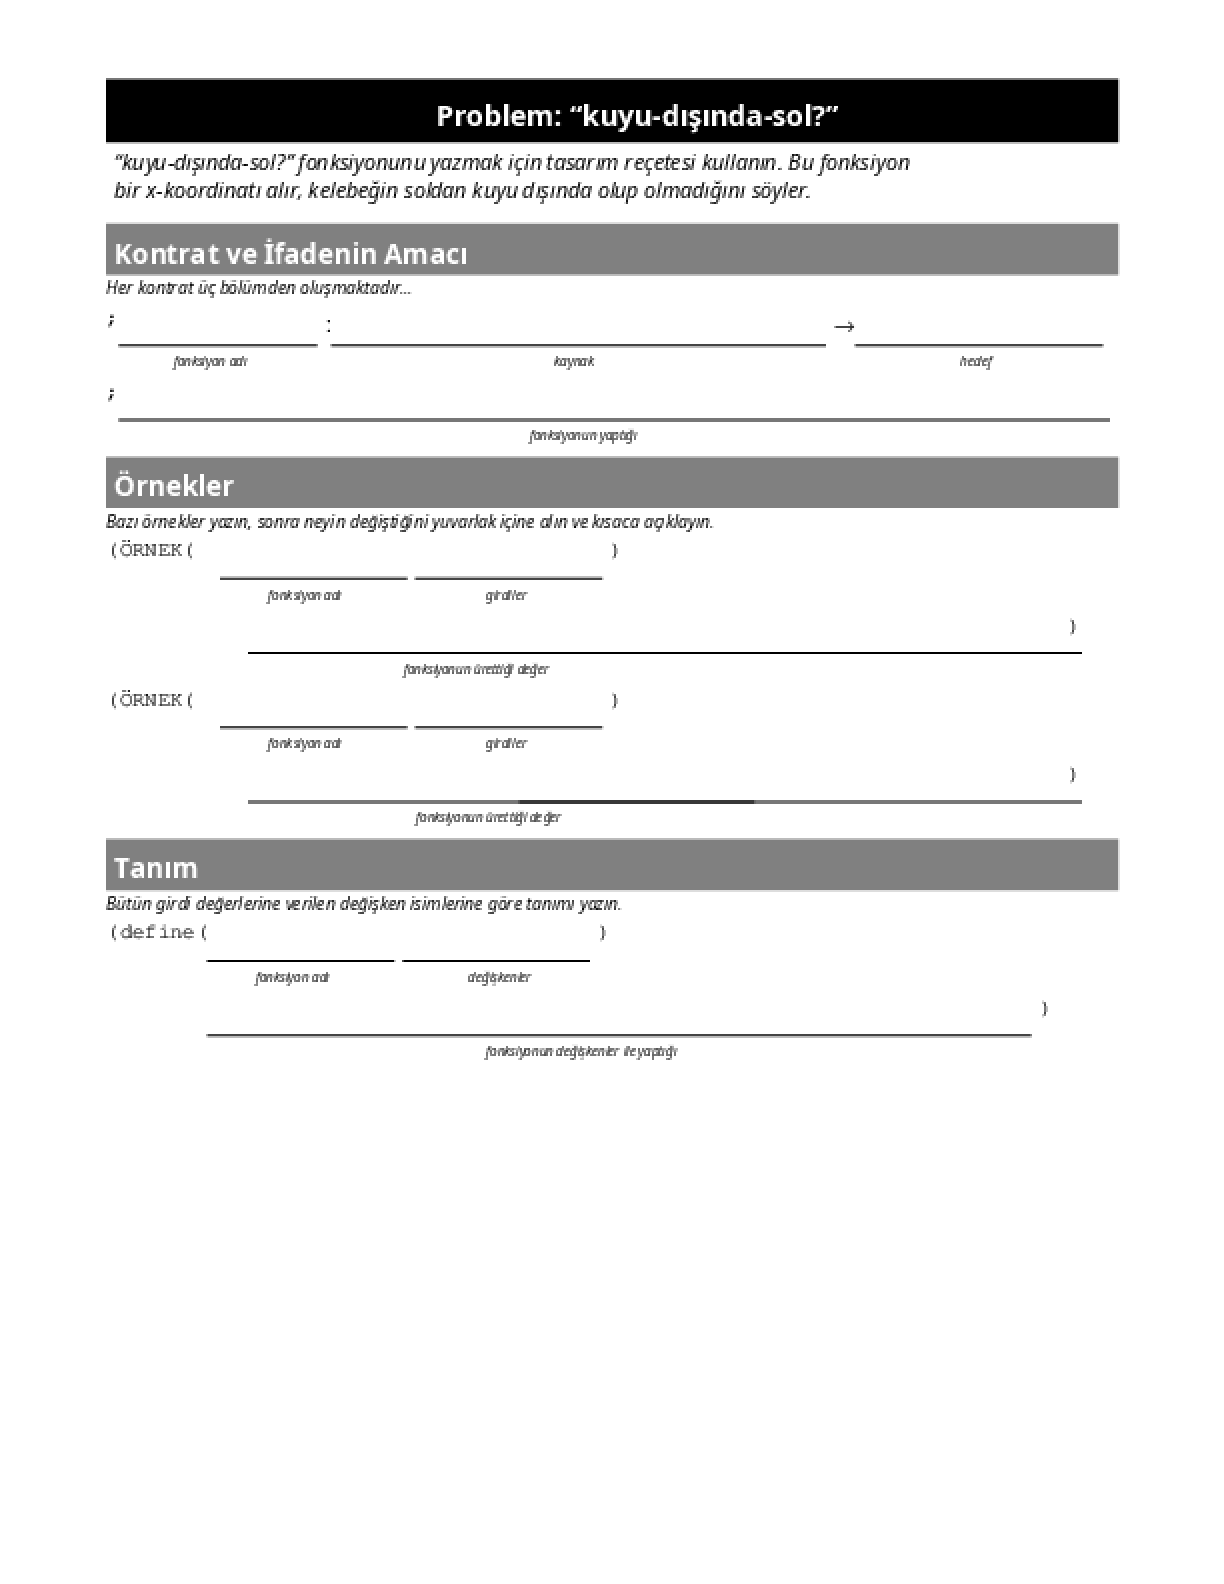
\includegraphics[width=1\linewidth]{cebirsplit-29.png}
\newpage
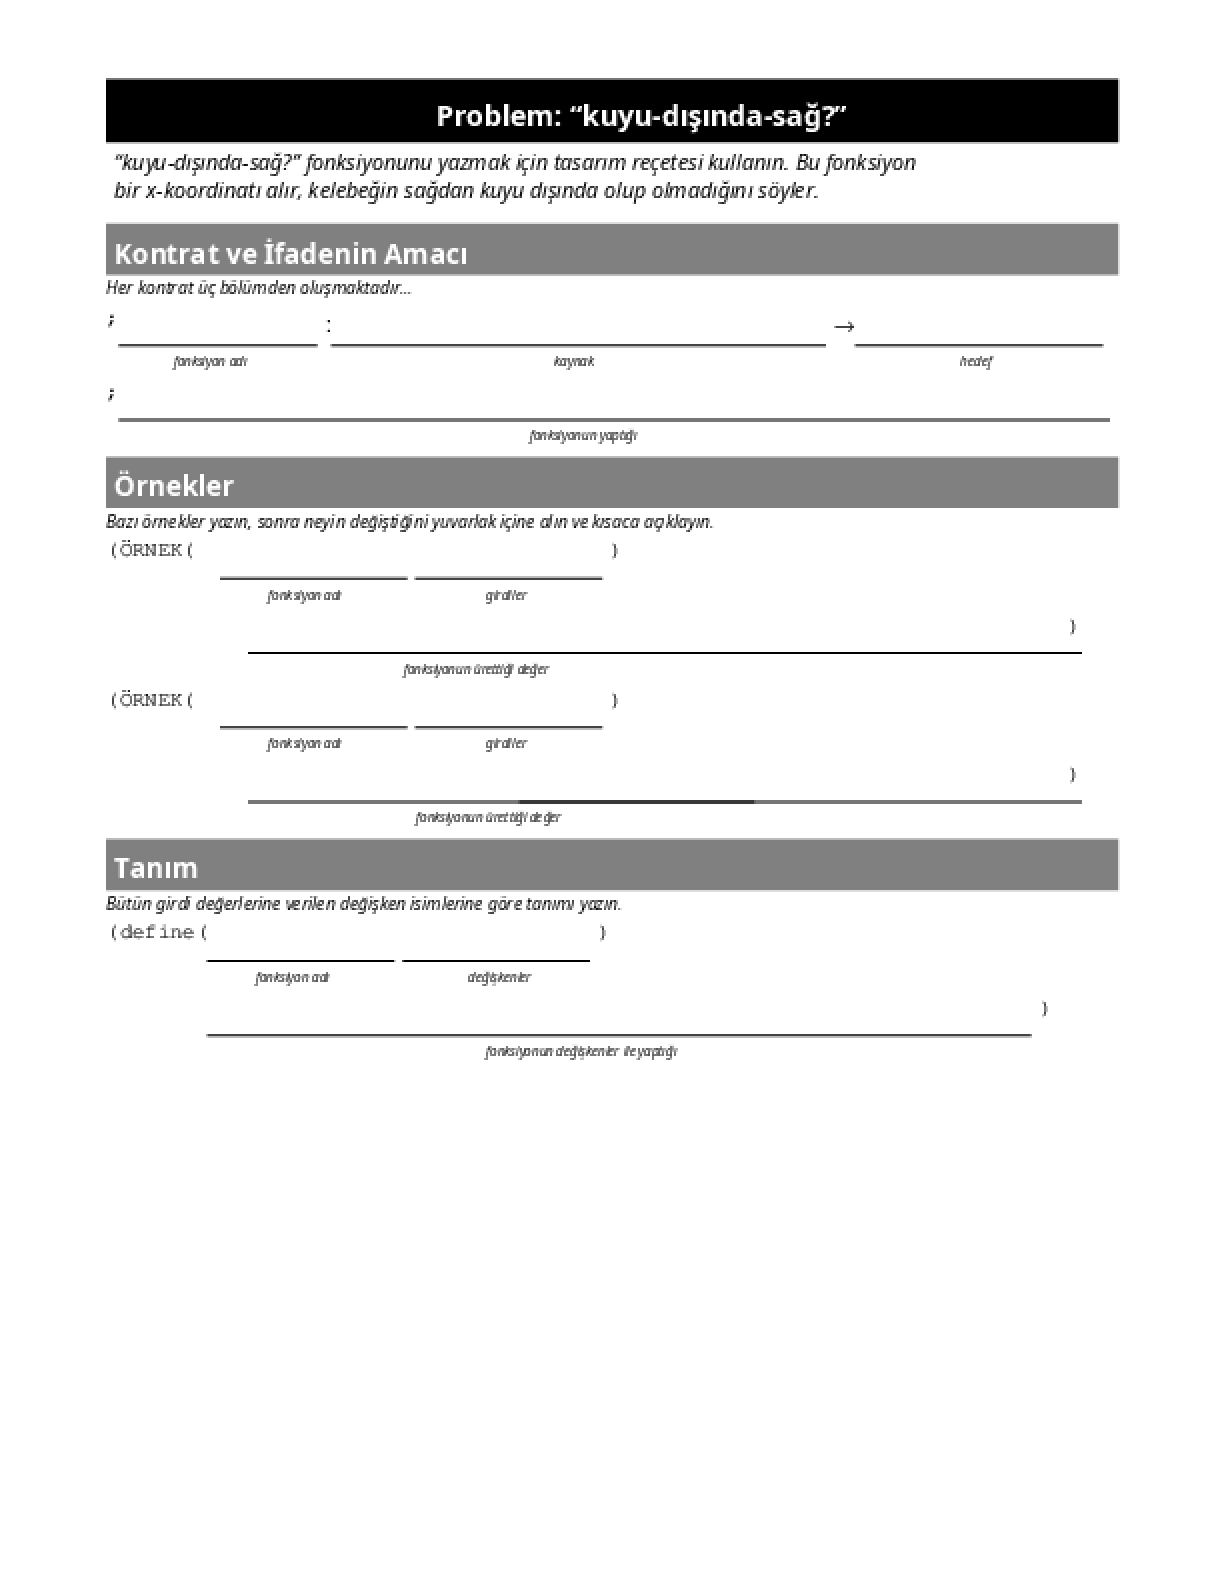
\includegraphics[width=1\linewidth]{cebirsplit-30.png}
\newpage
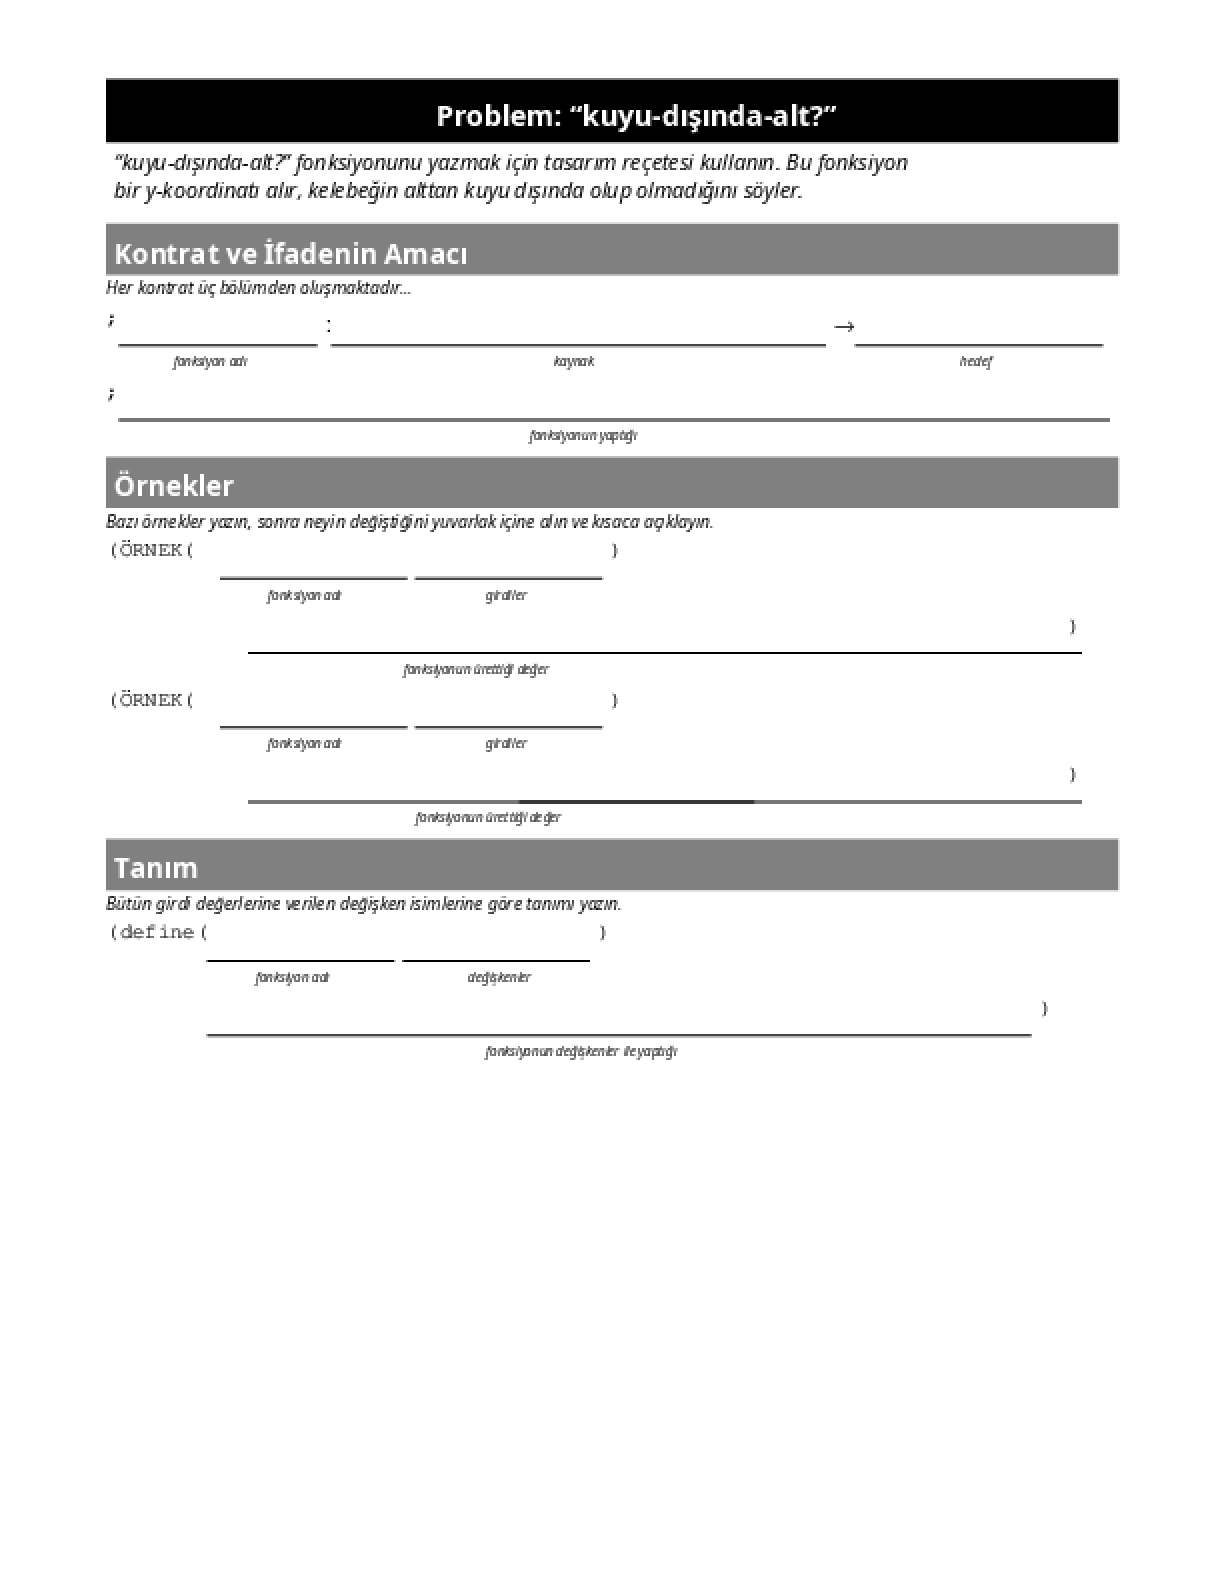
\includegraphics[width=1\linewidth]{cebirsplit-31.png}
\newpage
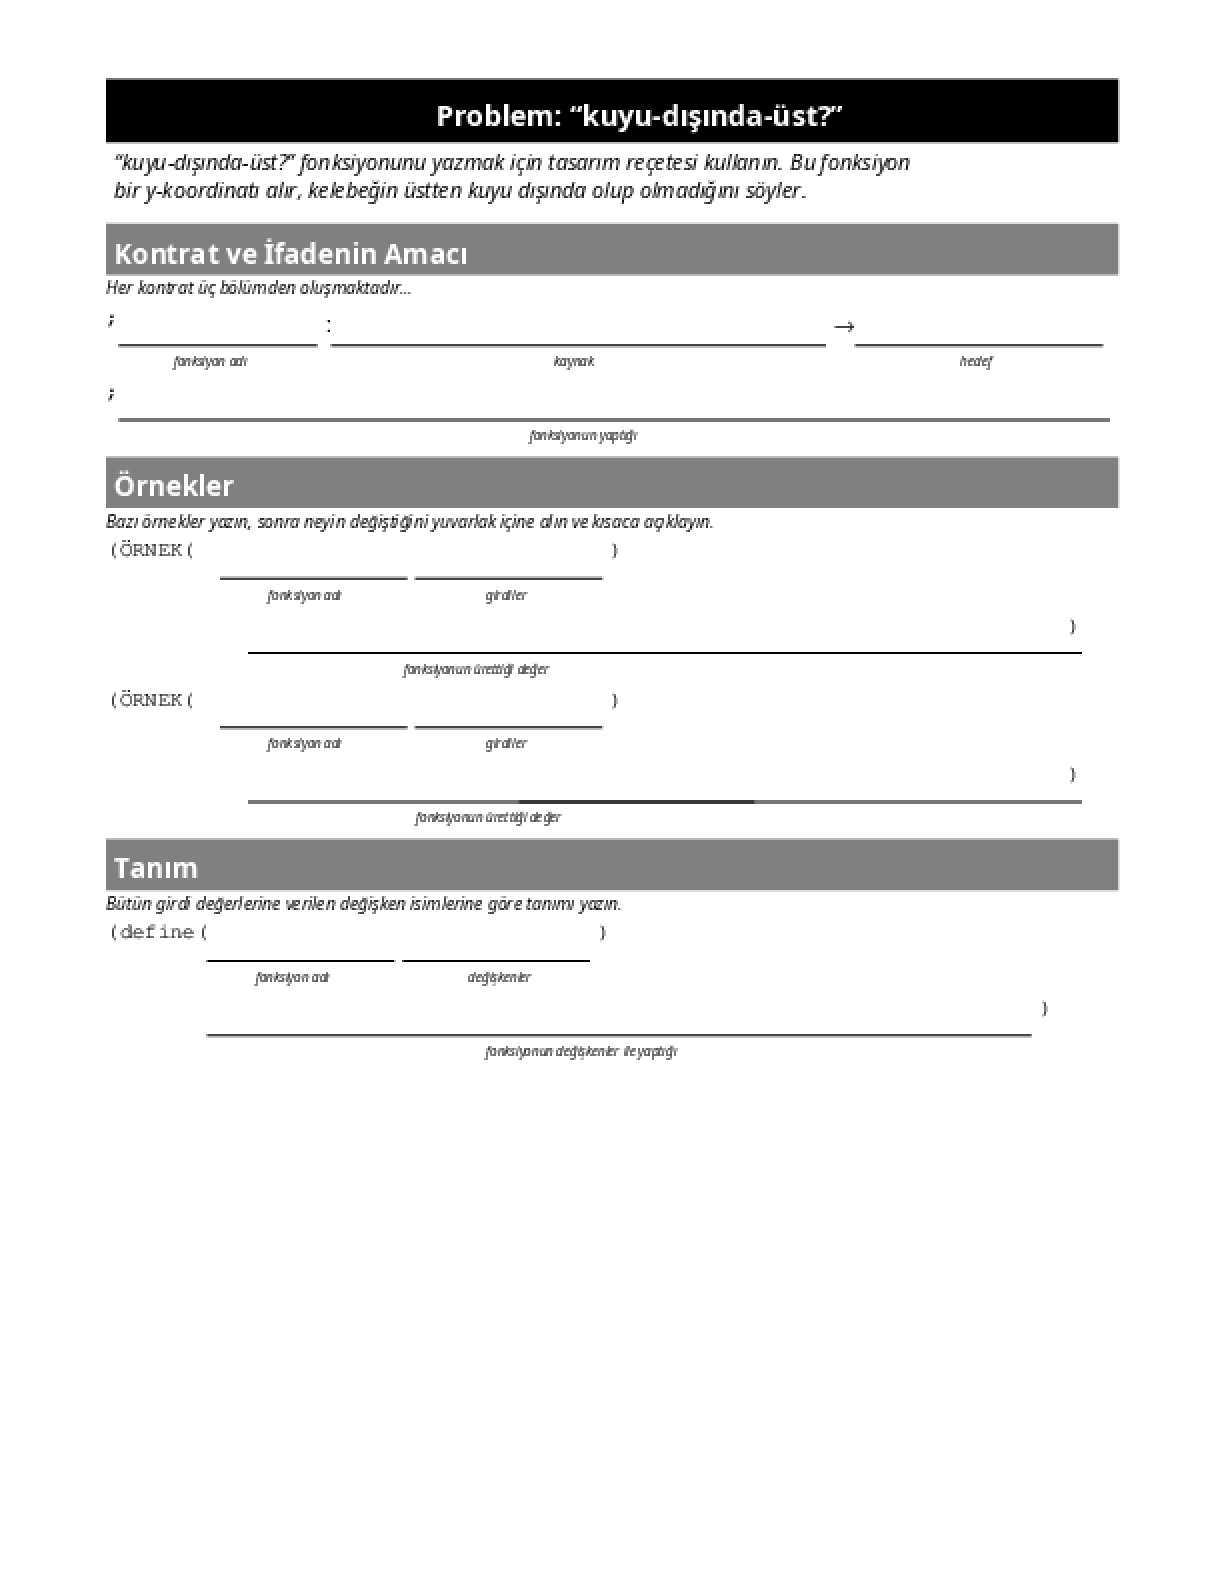
\includegraphics[width=1\linewidth]{cebirsplit-32.png}
\newpage
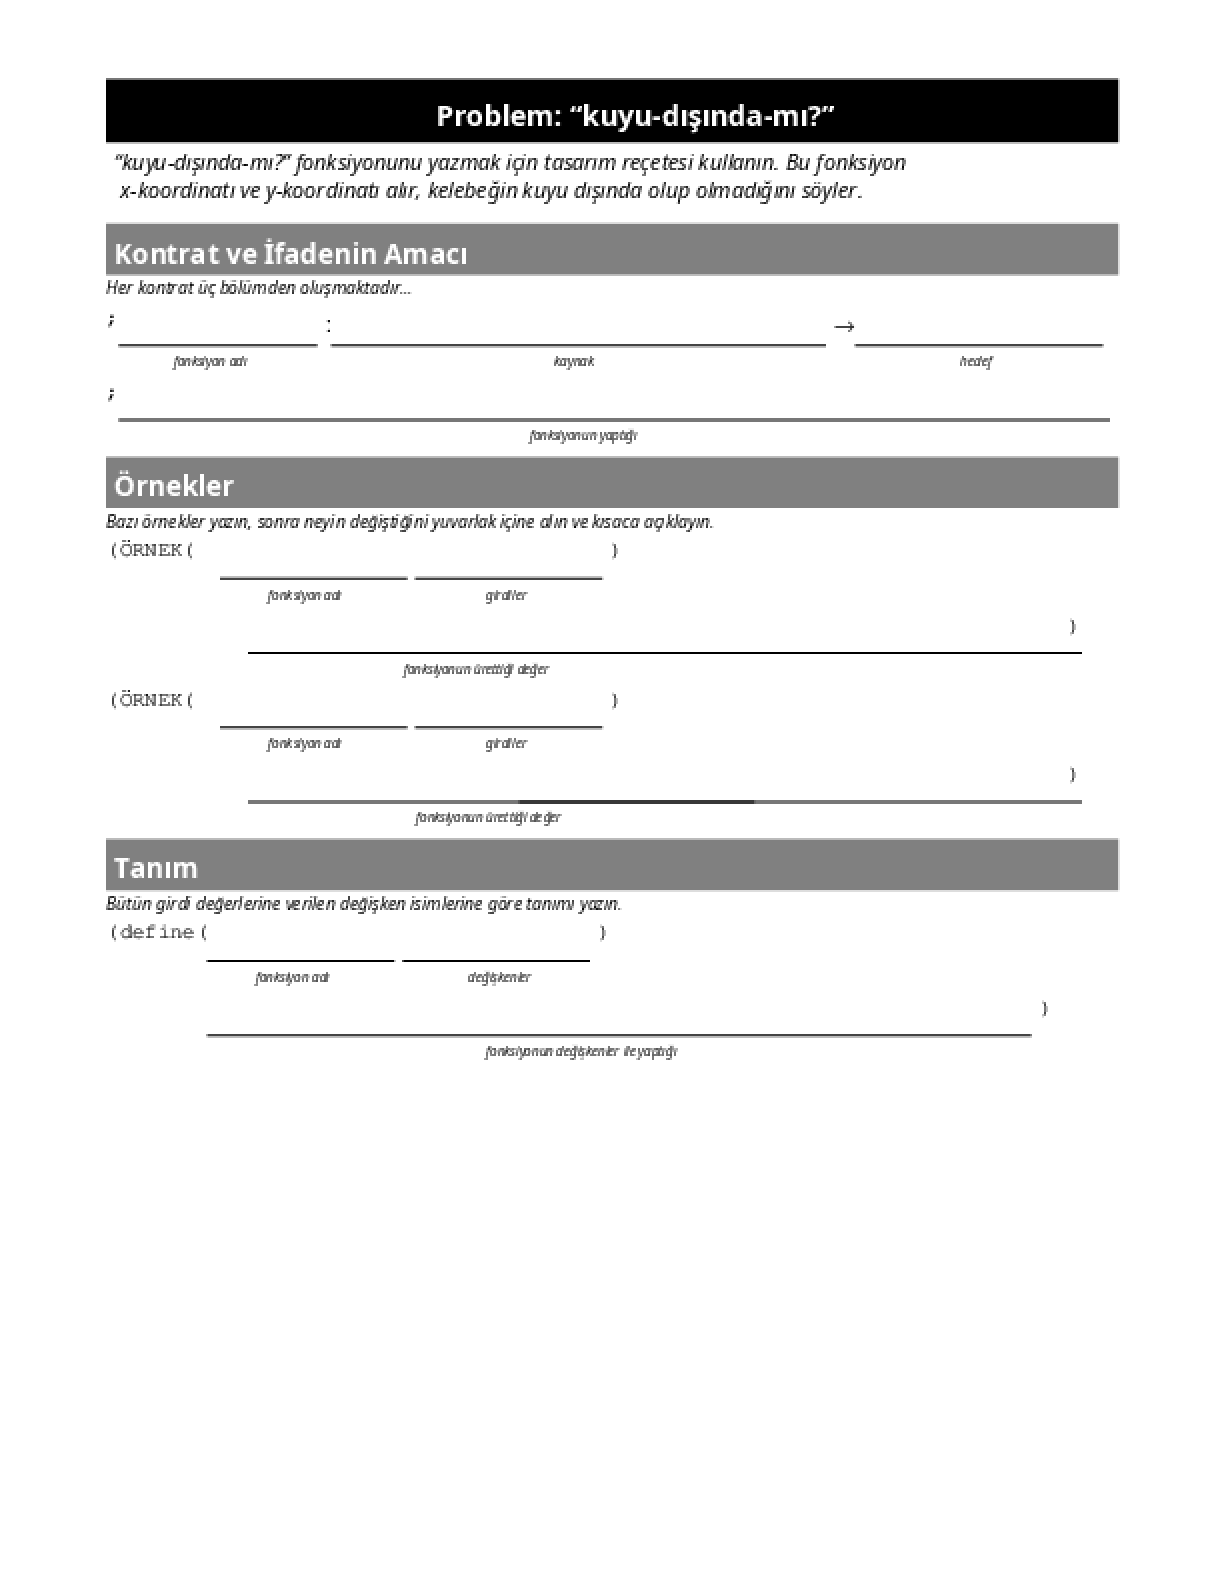
\includegraphics[width=1\linewidth]{cebirsplit-33.png}
\newpage
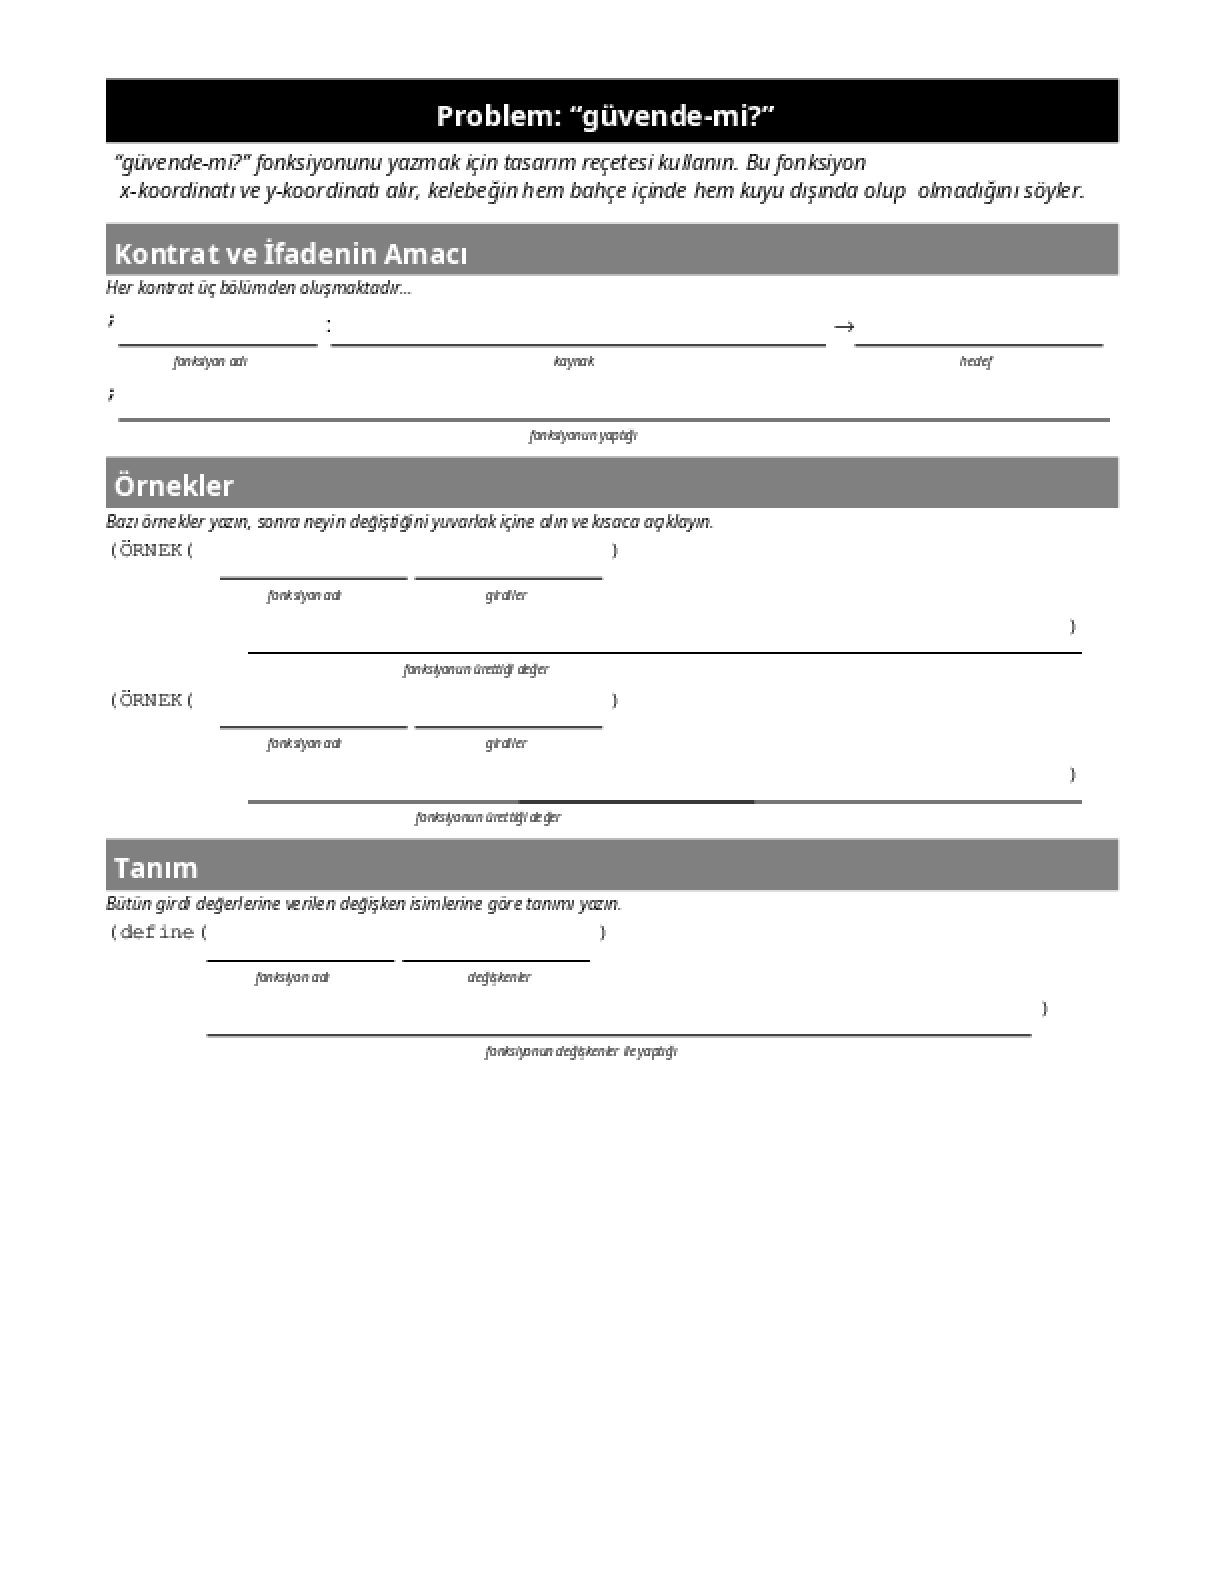
\includegraphics[width=1\linewidth]{cebirsplit-34.png}
\newpage
\includegraphics[width=1\linewidth]{cebirsplit-35.png}
\newpage
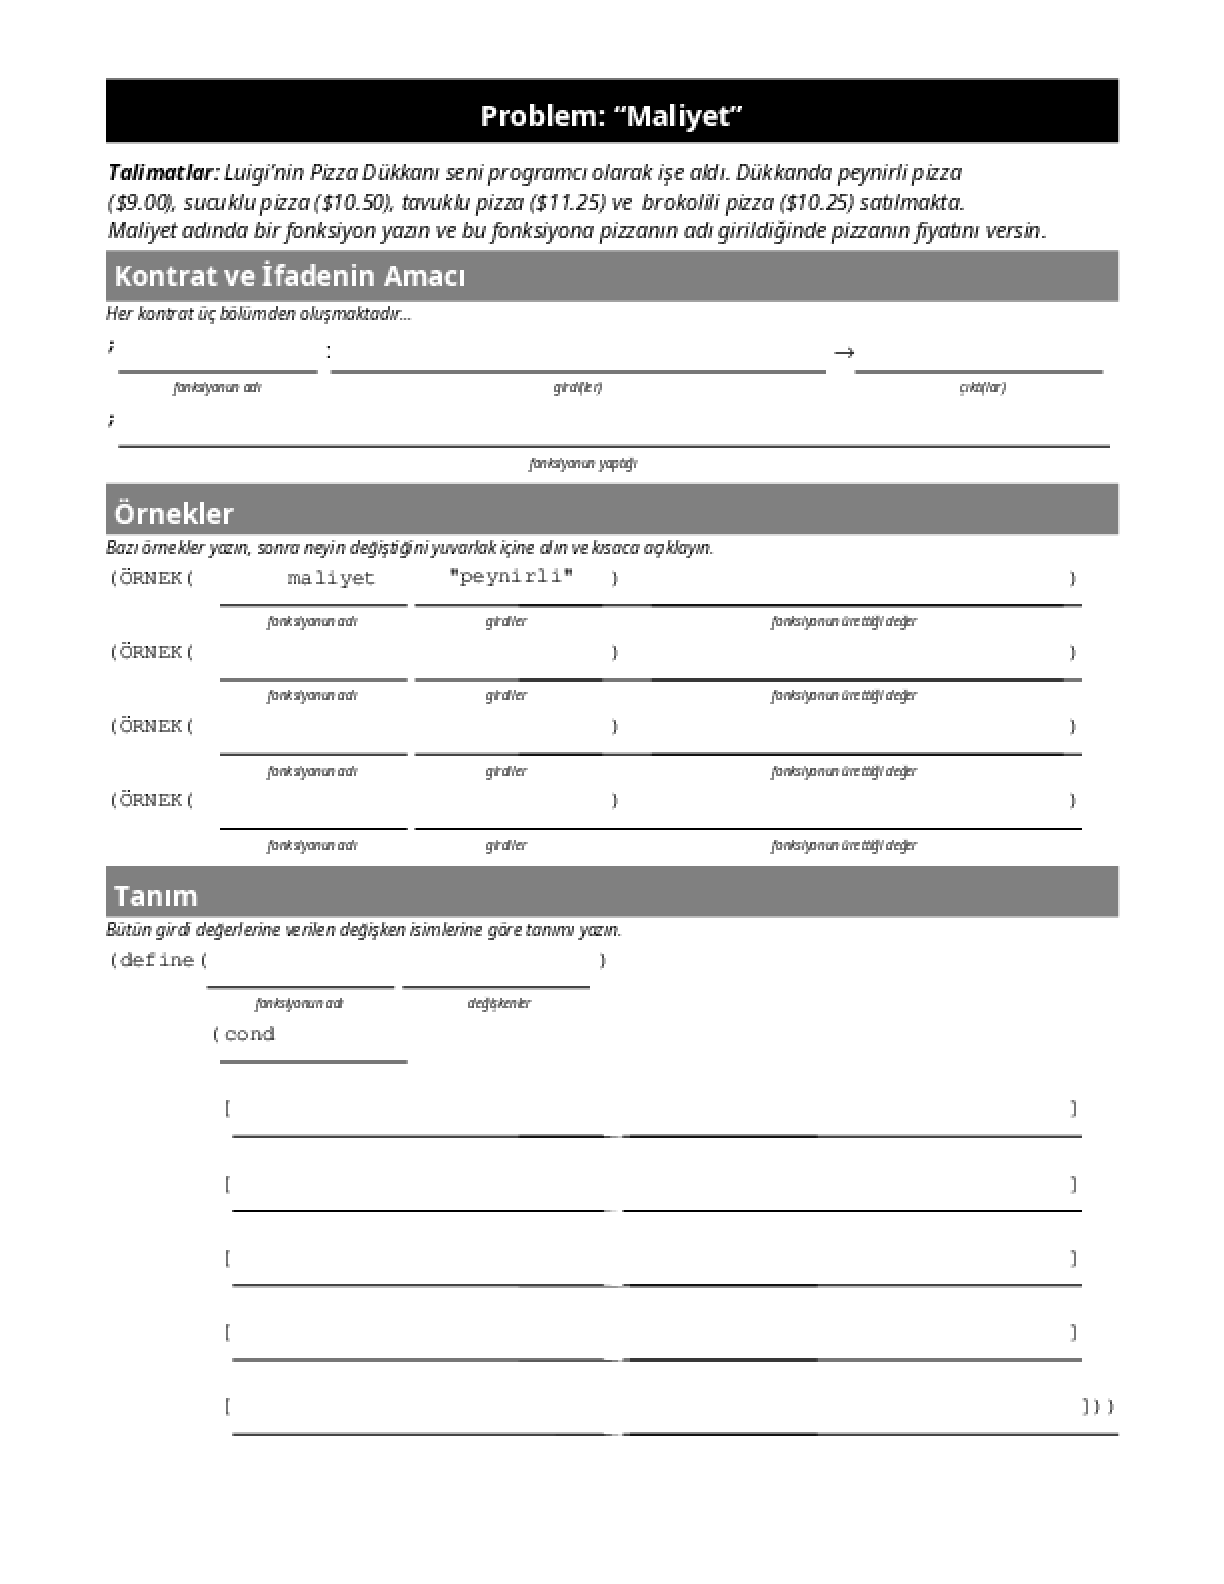
\includegraphics[width=1\linewidth]{cebirsplit-36.png}
\newpage
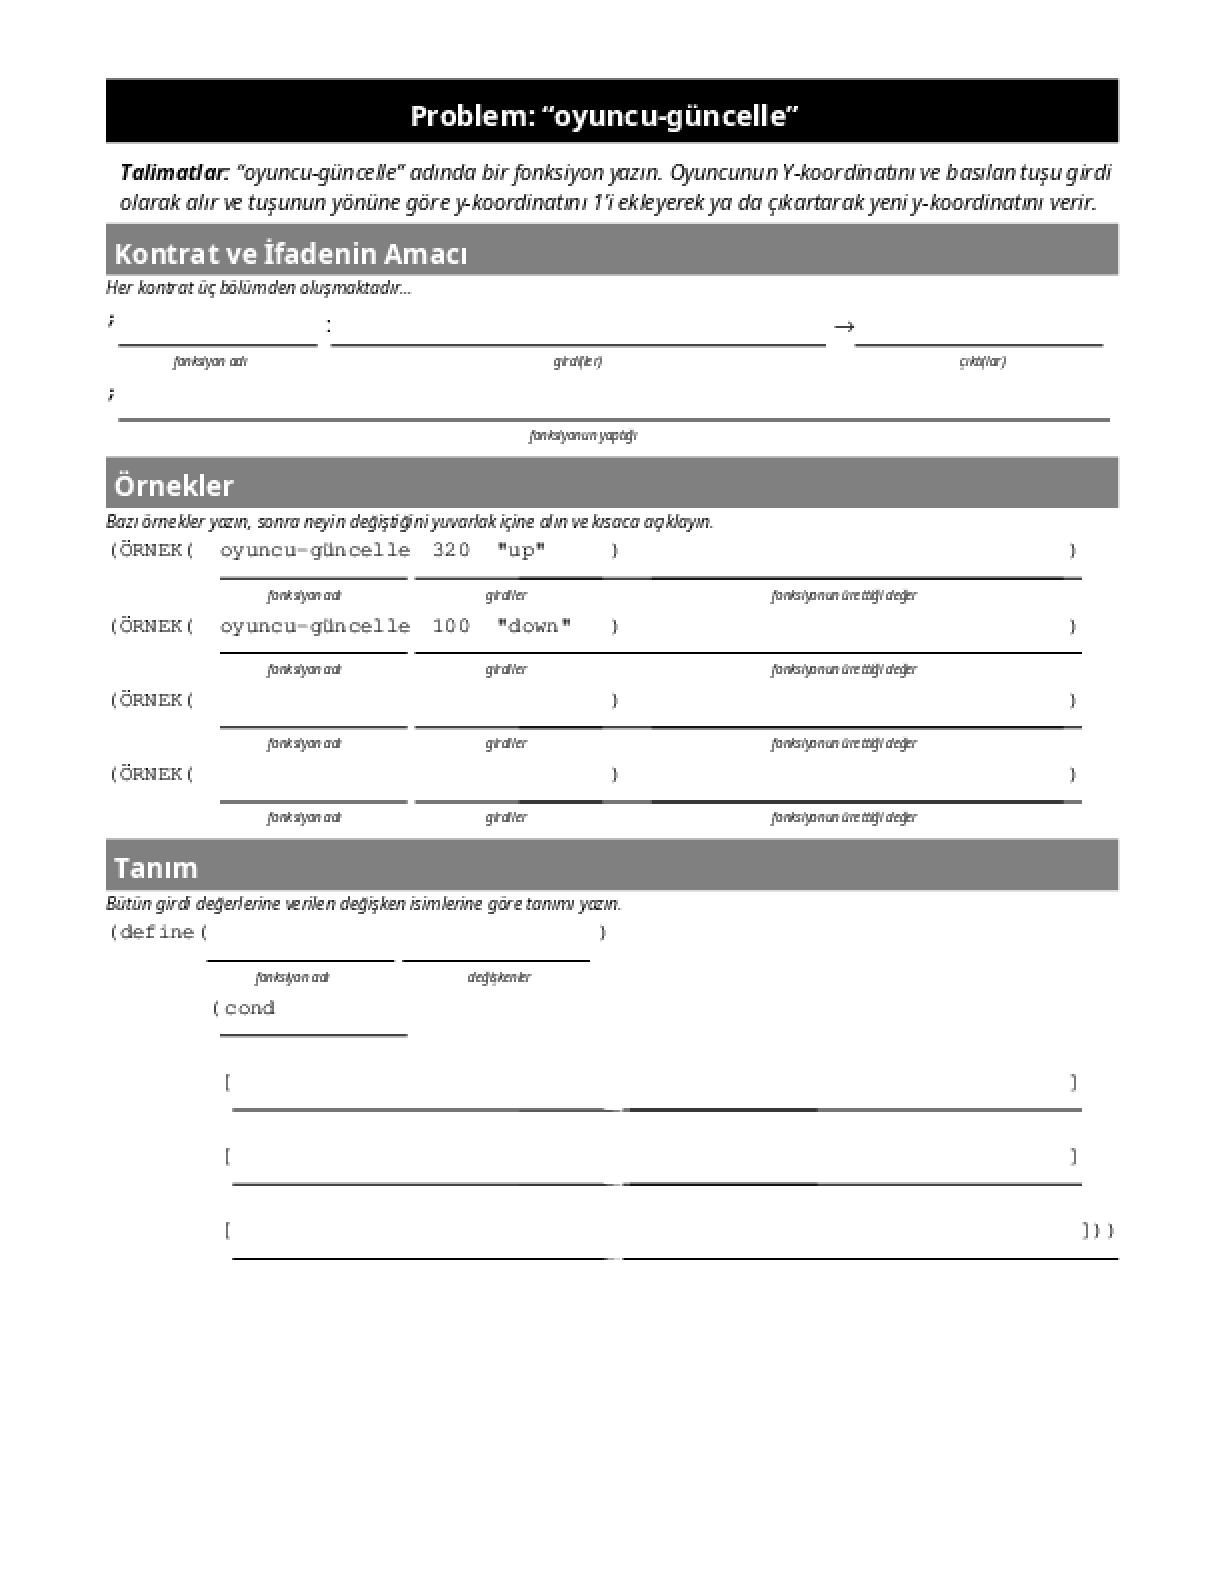
\includegraphics[width=1\linewidth]{cebirsplit-37.png}
\newpage
\includegraphics[width=1\linewidth]{cebirsplit-38.png}
\newpage
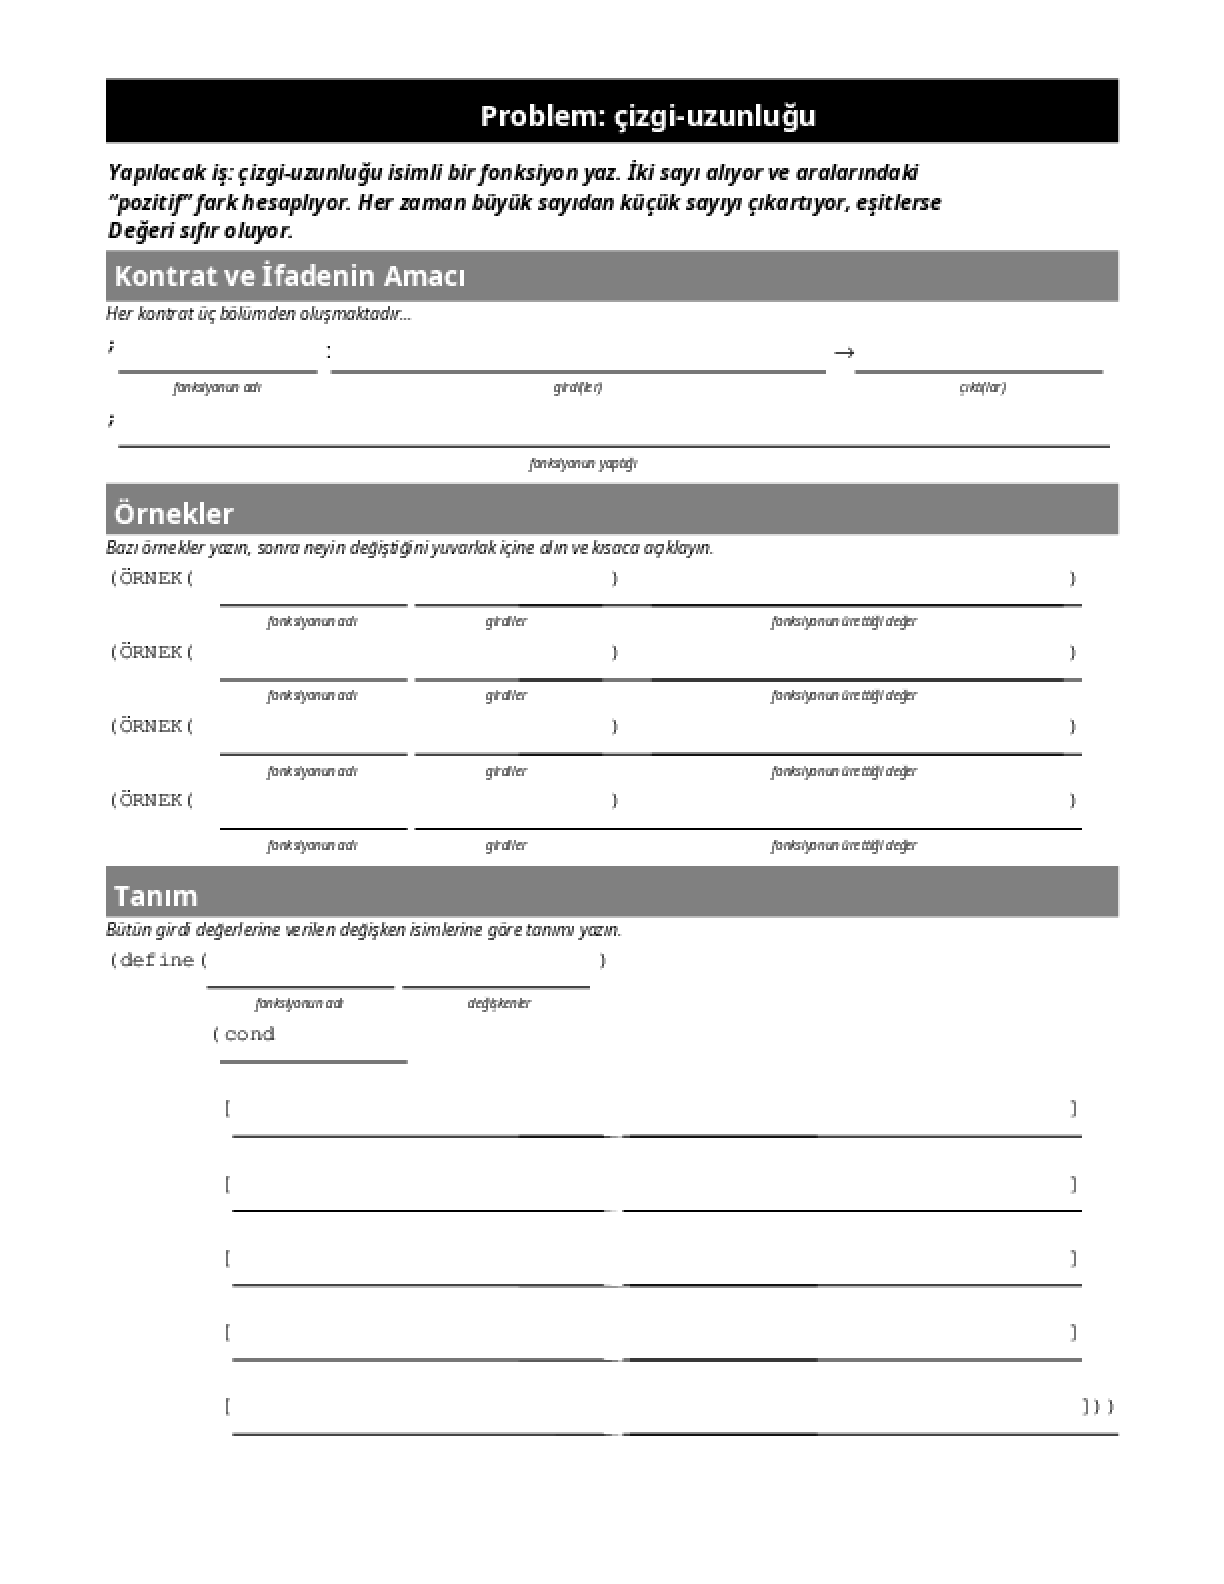
\includegraphics[width=1\linewidth]{cebirsplit-39.png}
\newpage
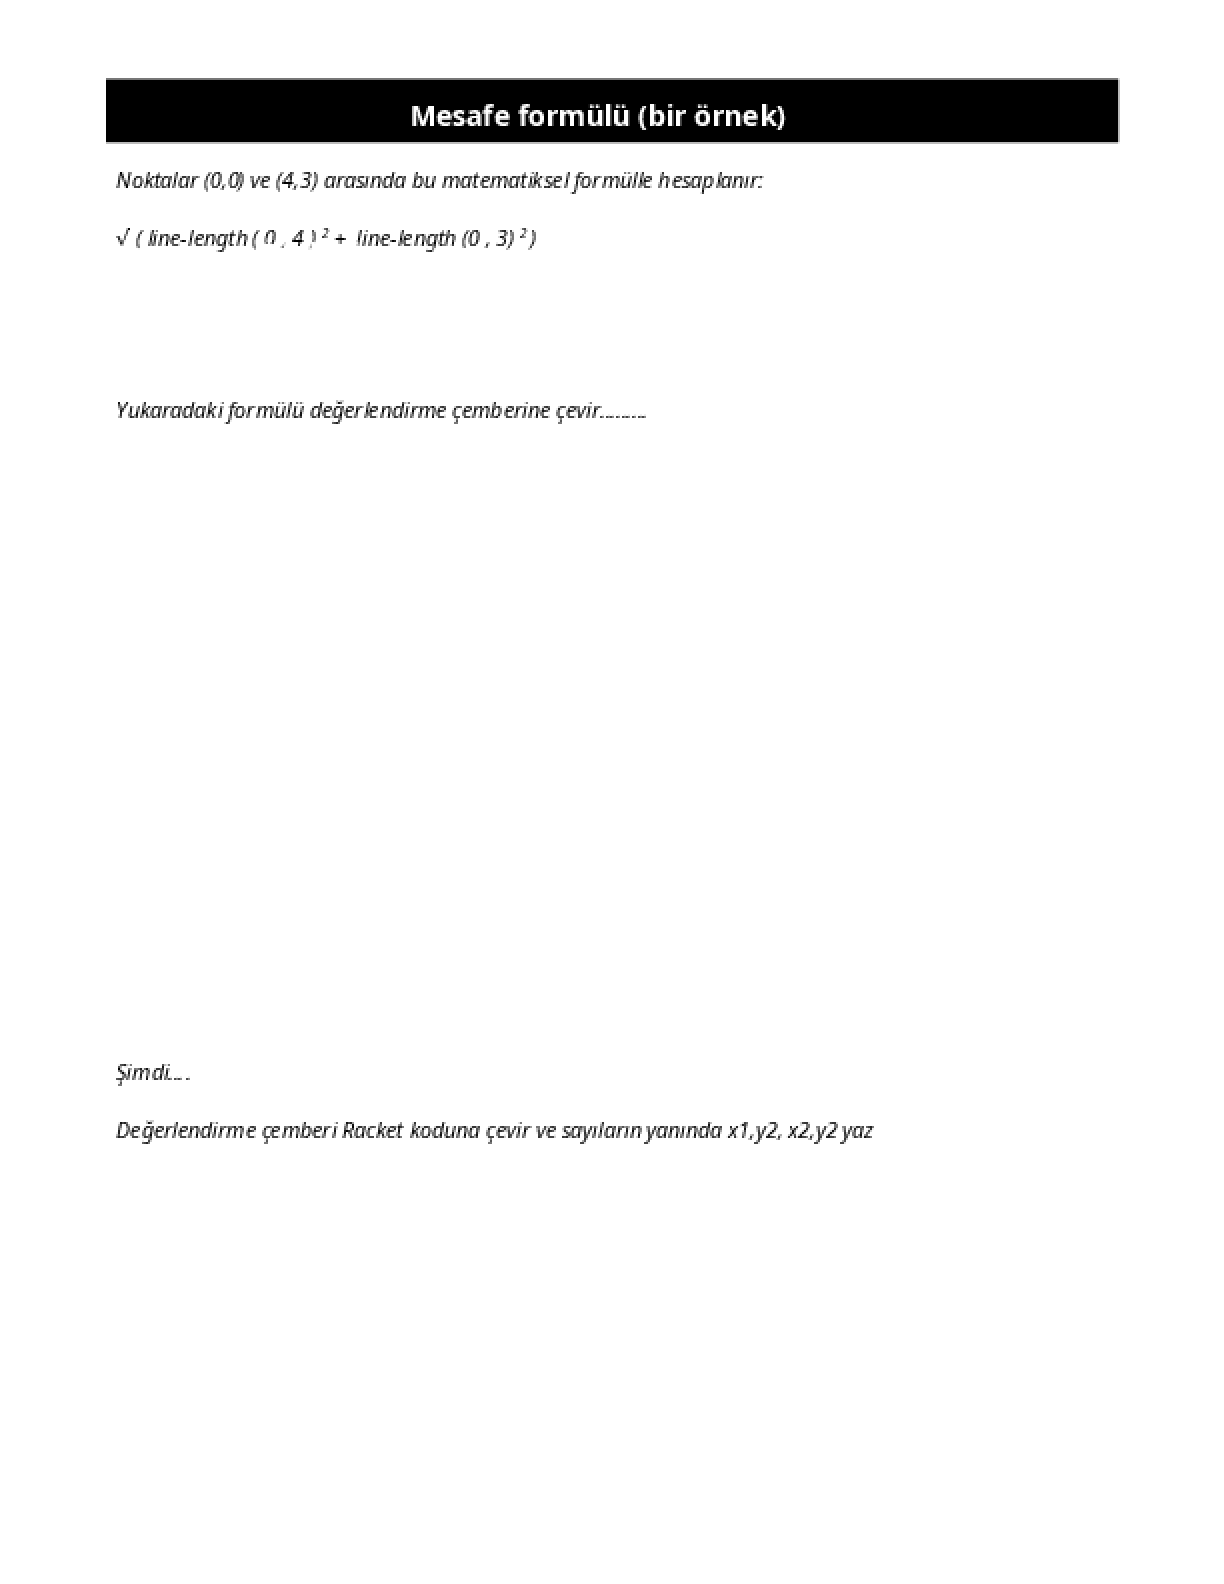
\includegraphics[width=1\linewidth]{cebirsplit-40.png}
\newpage
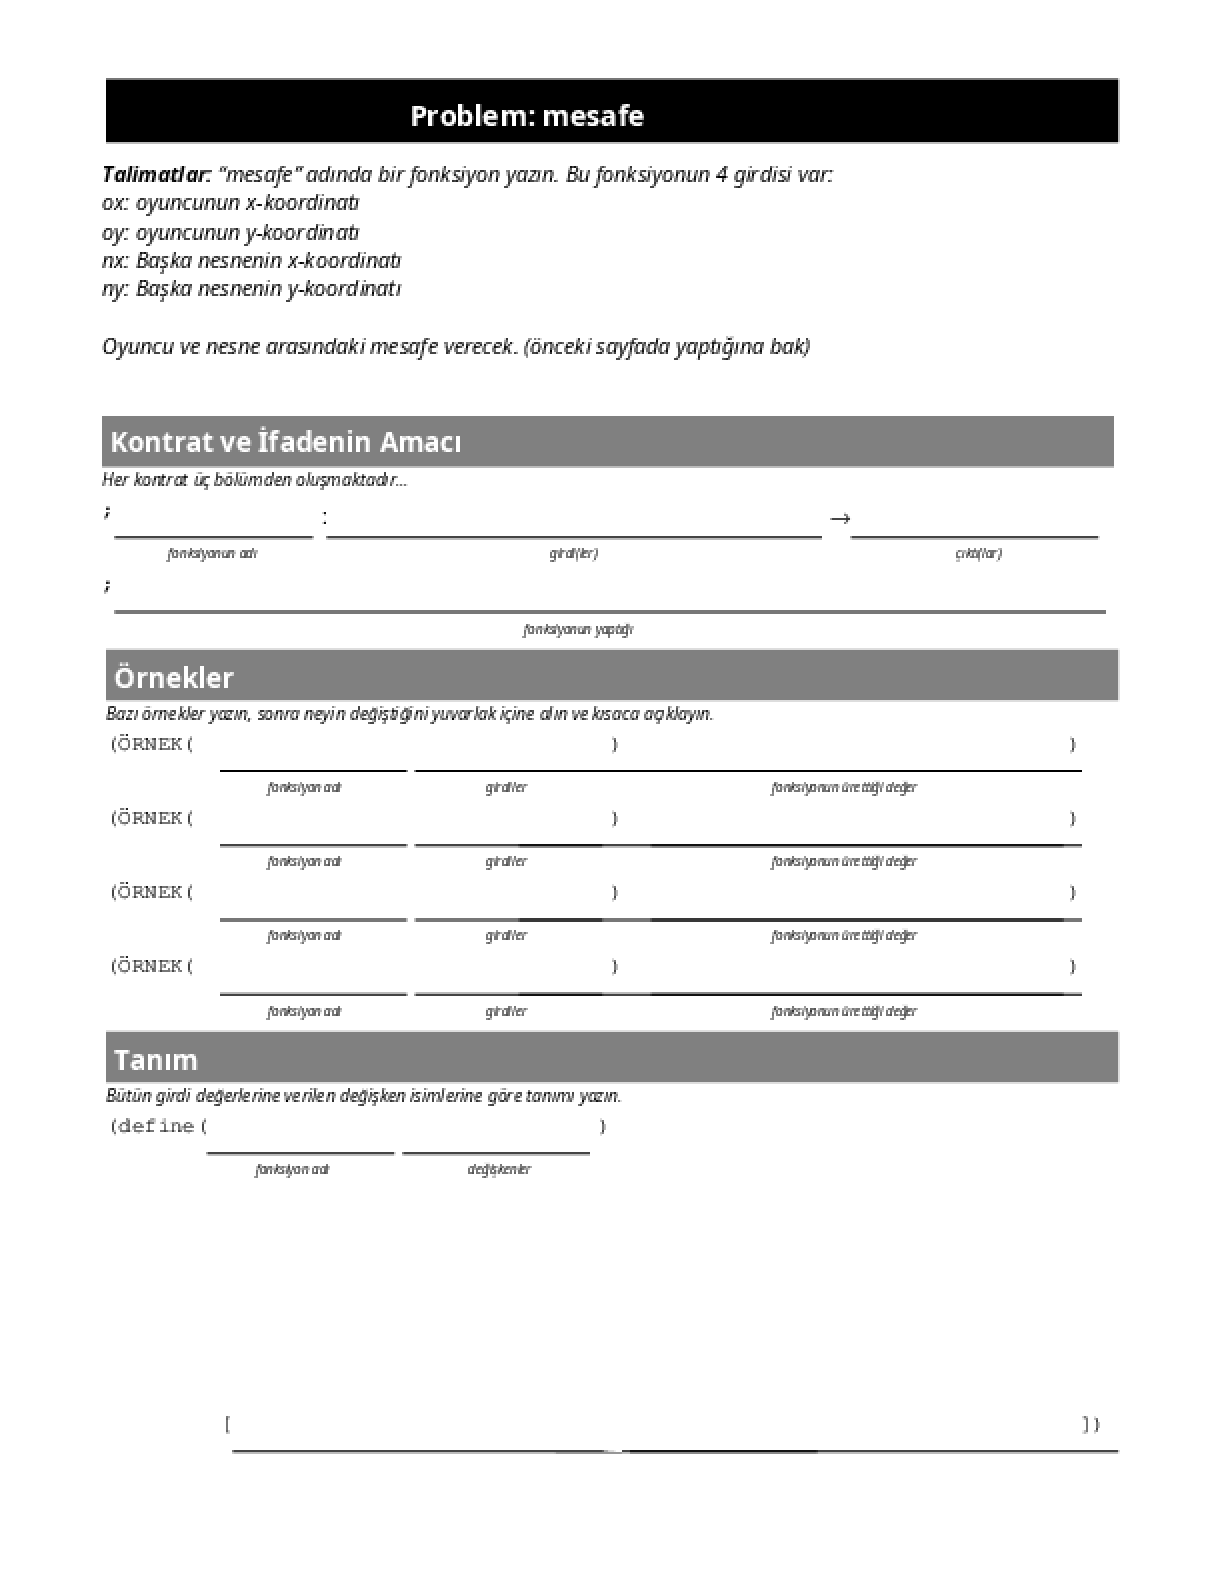
\includegraphics[width=1\linewidth]{cebirsplit-41.png}
\newpage
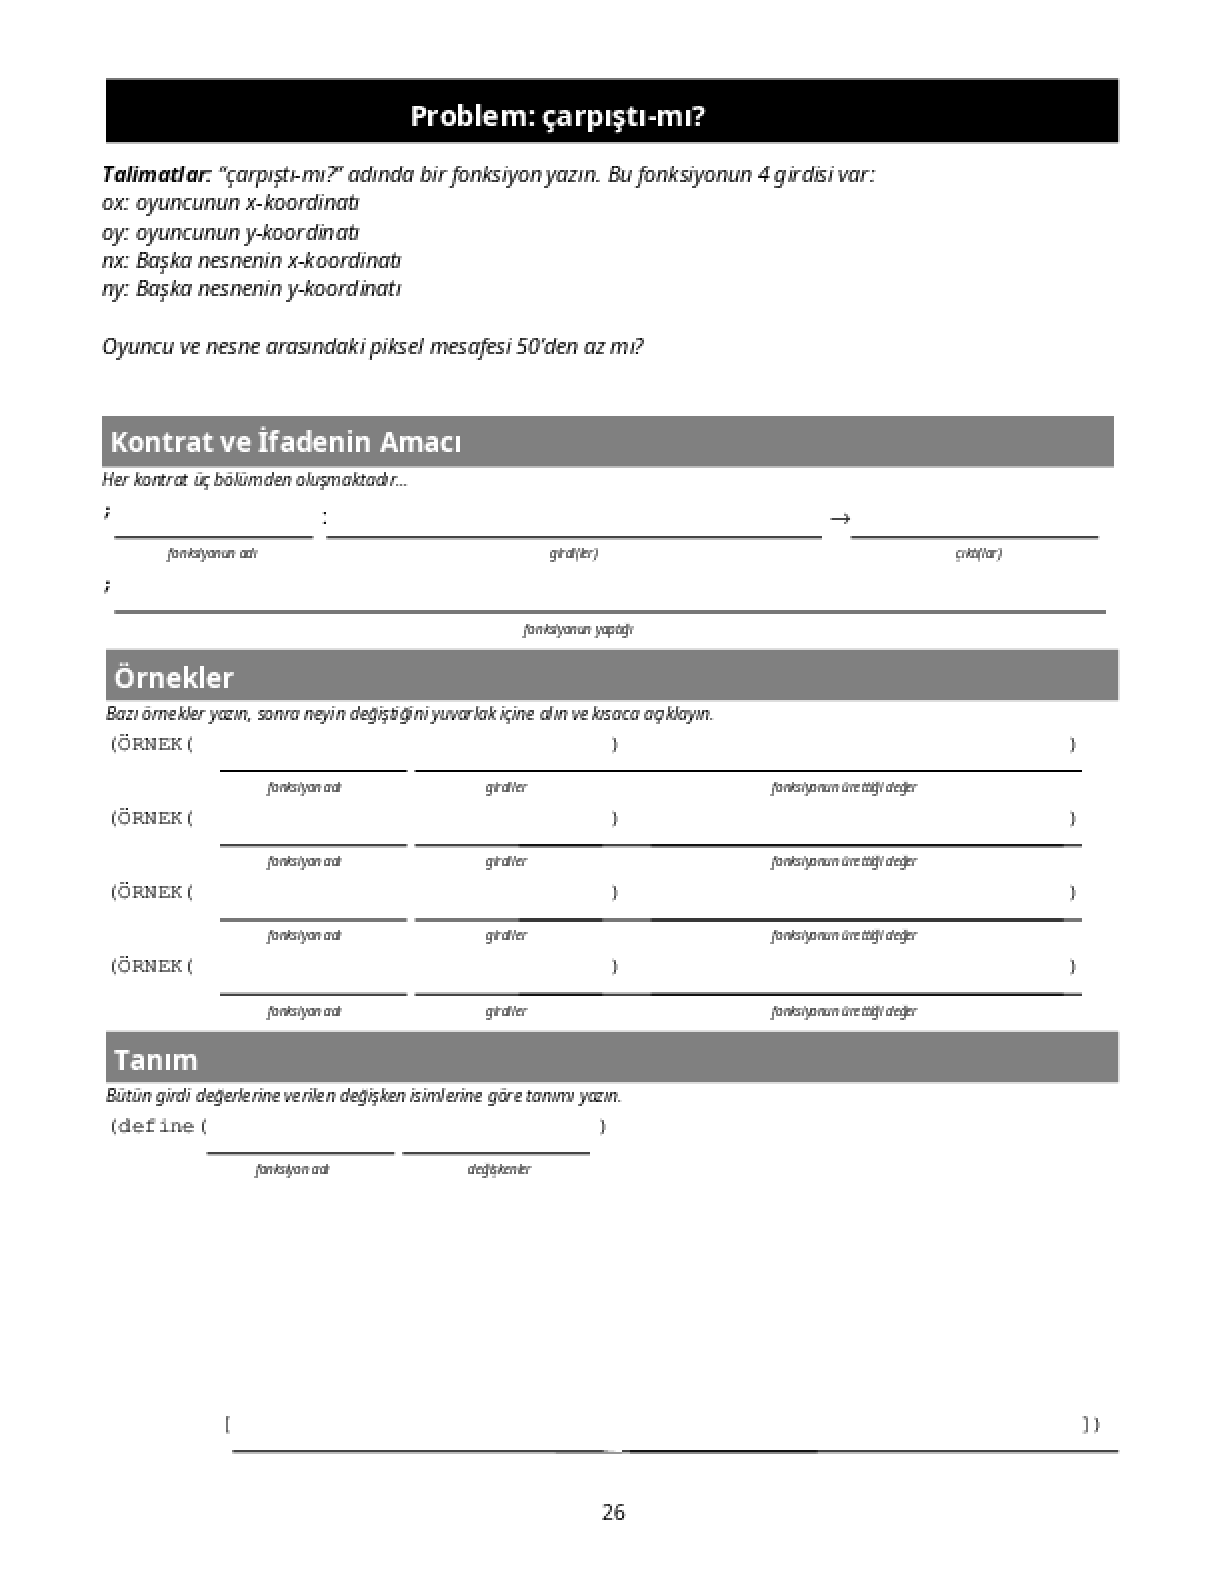
\includegraphics[width=1\linewidth]{cebirsplit-42.png}
\newpage
\includegraphics[width=1\linewidth]{cebirsplit-43.png}
\newpage
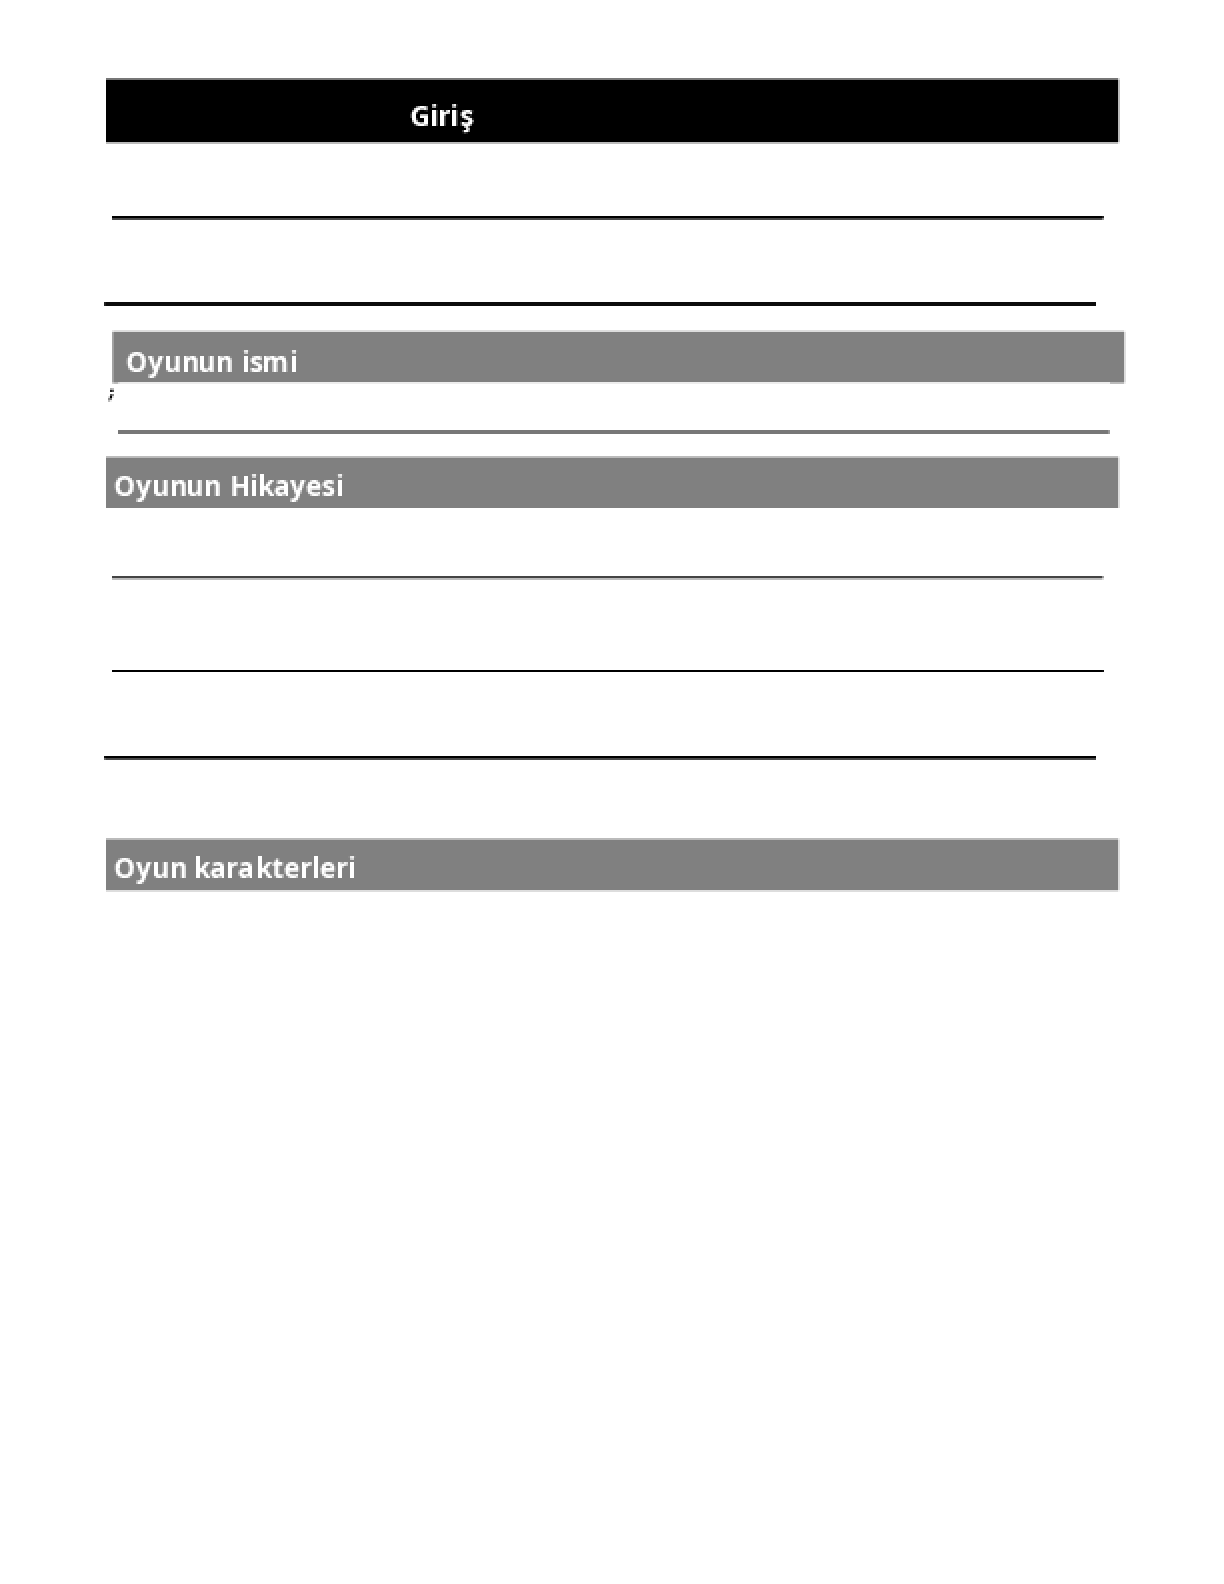
\includegraphics[width=1\linewidth]{cebirsplit-44.png}
\newpage
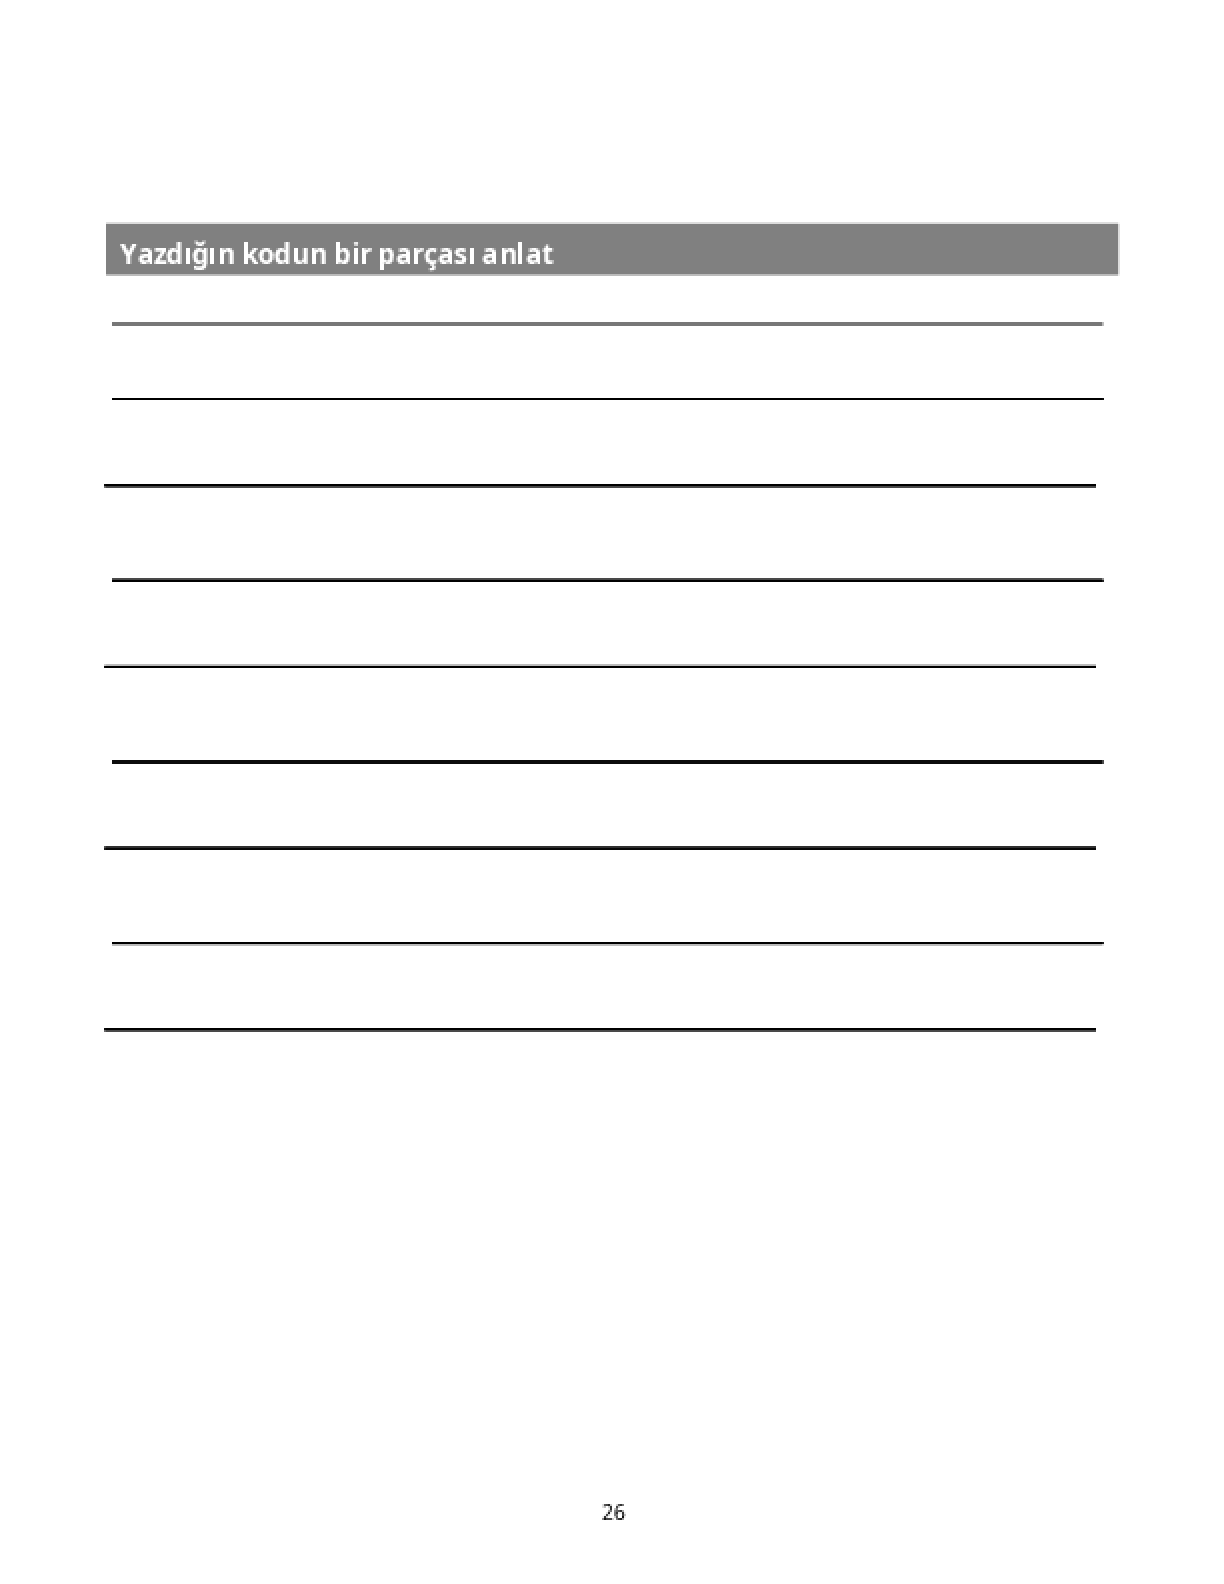
\includegraphics[width=1\linewidth]{cebirsplit-45.png}
\newpage
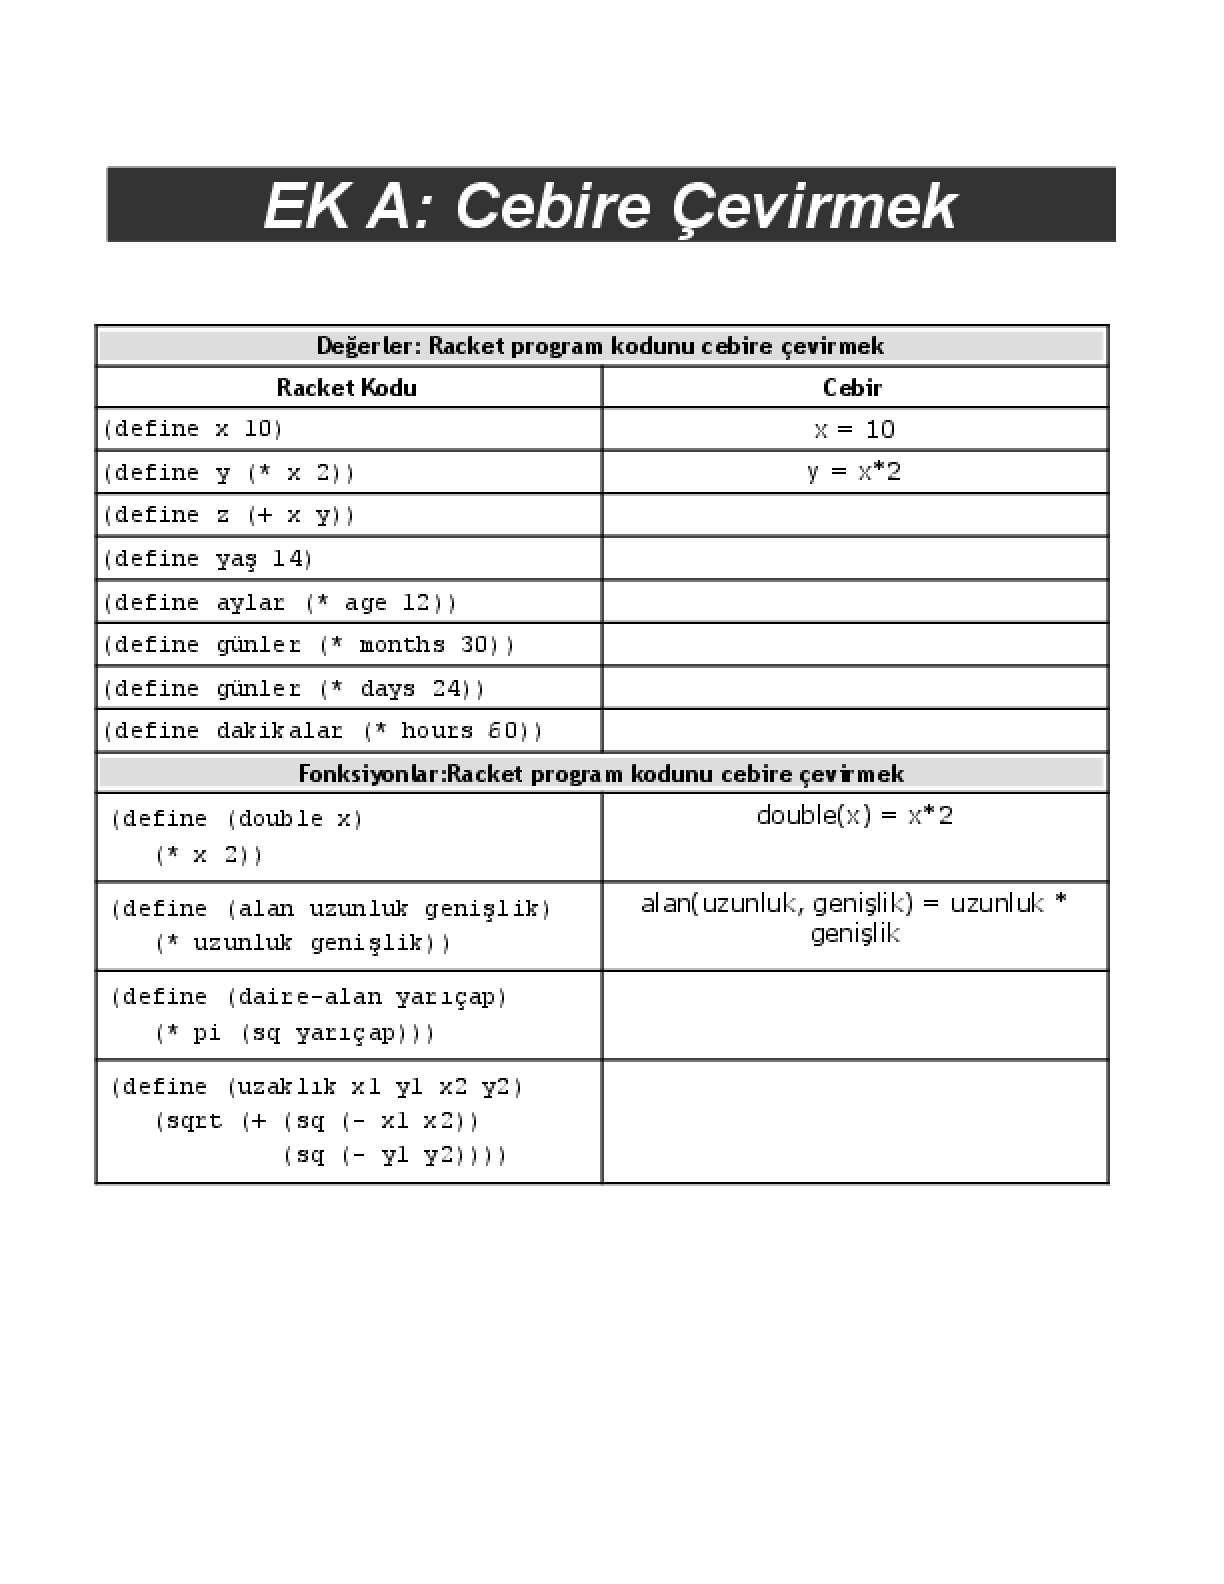
\includegraphics[width=1\linewidth]{cebirsplit-46.png}
\newpage
\includegraphics[width=1\linewidth]{cebirsplit-47.png}
\newpage
\includegraphics[width=1\linewidth]{cebirsplit-48.png}
\newpage
\includegraphics[width=1\linewidth]{cebirsplit-49.png}
\newpage
\includegraphics[width=1\linewidth]{cebirsplit-50.png}
\newpage
\includegraphics[width=1\linewidth]{cebirsplit-51.png}
\newpage
\includegraphics[width=1\linewidth]{cebirsplit-52.png}
\newpage
\includegraphics[width=1\linewidth]{cebirsplit-53.png}
\newpage
\includegraphics[width=1\linewidth]{cebirsplit-54.png}
\newpage
\includegraphics[width=1\linewidth]{cebirsplit-55.png}
\newpage

\setcounter{page}{57}
%\noindent {\large \bf Ad/Soyadı3: \dotfill}\\
\vspace*{0.8cm}
\begin{center}
\includegraphics[width=0.8\linewidth]{reactive.png}

\includegraphics[width=0.25\linewidth]{bootstrap-logo.png}
 
\end{center}

\vspace*{0.2cm}


\begin{center}
{\Large \bf{Nesin Köyleri Cebir ve Programlama Yazokulu 2024 - Evren}}

{\tiny Bootstrap is licensed under a Creative Commons 3.0 Unported License. Based on a work from
www.BootstrapWorld.org. Permissions beyond the scope of this license may be available at
contact@BootstrapWorld.org.

Türkçe versiyonu. Mehmet Gençer, Chris Stephenson ve diğer Nesin Köyleri Cebir ve Programlama Yazokulu öğretim takım üyeleri.

Lisans: Creative Commons 3.0 Unported License} 
\end{center}


\newpage

\subsection*{Veri Yapı Tasarımı}
İsim \fillin[5cm]pasta\\
\vspace{0.5cm}\\
\begin{tabular}{| p{4cm} | p{4cm} | p{8cm} |  }
\hline			
Komponent ismi&Komponent veri tipi&Anlam\\
\hline
renk&color &pastanın rengi \\[10ex]
\hline  
mesaj-rengi&color &mesajın rengi \\[10ex]
\hline  
kat&sayı &pasta katların sayısı \\[10ex]
\hline  
mesaj&metin &pasta üstündeki mesaj \\[10ex]
\hline  
yarı-çap&sayı &pastanın yarı çapı \\[10ex]
\hline  
\end{tabular}

\subsubsection*{Tanım}
\begin{tabular}{| p{17cm} |  }
\hline			
\vspace{0.5cm}
(STRUCT \fillin[3cm]pasta (\fillin[1cm]renk kat mesaj mesaj-rengi yarı-çap ))\\[10ex]
\hline
\end{tabular}





\newpage
\subsection*{Tasarım Recetesi}
\subsubsection*{Sözleşme}
\begin{tabular}{| p{4cm} | p{8cm} | p{4cm} |  }
\hline			
Fonksiyon ismi&Giriş veri tip(ler)i&Sonuç veri tipi\\
\hline
isim-ekle& & \\[10ex]
\hline  
\end{tabular}

\subsubsection*{Amaç}
\begin{tabular}{| p{17cm} |  }
\hline			
Amaç\\
\hline
 \\[10ex]
\hline  
\end{tabular}

\subsubsection*{Örnekler}
\begin{tabular}{| p{4cm} | p{8cm} | p{4cm} |  }
\hline			
Fonksiyon ismi&Giriş veri(ler)i&Sonuç veri\\
\hline
& & \\[6ex]
\hline  
& & \\[6ex]
\hline  
& & \\[6ex]
\hline  
& & \\[6ex]
\hline  
\end{tabular}

\subsubsection*{Şablon}
\begin{tabular}{| p{17cm} |  }
\hline			
Şablon\\
\hline
\vspace{0,2cm}
(define (\fillin[2cm] \hspace{1cm}  \fillin[8cm] ) \\[30ex]
\hline  
\end{tabular}

\newpage
\subsection*{Tasarım Recetesi}
\subsubsection*{Sözleşme}
\begin{tabular}{| p{4cm} | p{8cm} | p{4cm} |  }
\hline			
Fonksiyon ismi&Giriş veri tip(ler)i&Sonuç veri tipi\\
\hline
scale-pasta& & \\[10ex]
\hline  
\end{tabular}

\subsubsection*{Amaç}
\begin{tabular}{| p{17cm} |  }
\hline			
Amaç\\
\hline
 \\[10ex]
\hline  
\end{tabular}

\subsubsection*{Örnekler}
\begin{tabular}{| p{4cm} | p{8cm} | p{4cm} |  }
\hline			
Fonksiyon ismi&Giriş veri(ler)i&Sonuç veri\\
\hline
& & \\[6ex]
\hline  
& & \\[6ex]
\hline  
& & \\[6ex]
\hline  
& & \\[6ex]
\hline  
\end{tabular}

\subsubsection*{Şablon}
\begin{tabular}{| p{17cm} |  }
\hline			
Şablon\\
\hline
\vspace{0,5cm}
\vspace{0,2cm}
(define (\fillin[2cm] \hspace{1cm}  \fillin[8cm] ) \\[30ex]
\hline  
\end{tabular}

\newpage
\subsection*{Tasarım Recetesi}
\subsubsection*{Sözleşme}
\begin{tabular}{| p{4cm} | p{8cm} | p{4cm} |  }
\hline			
Fonksiyon ismi&Giriş veri tip(ler)i&Sonuç veri tipi\\
\hline
çift-kat& & \\[10ex]
\hline  
\end{tabular}

\subsubsection*{Amaç}
\begin{tabular}{| p{17cm} |  }
\hline			
Amaç\\
\hline
 \\[10ex]
\hline  
\end{tabular}

\subsubsection*{Örnekler}
\begin{tabular}{| p{4cm} | p{8cm} | p{4cm} |  }
\hline			
Fonksiyon ismi&Giriş veri(ler)i&Sonuç veri\\
\hline
& & \\[6ex]
\hline  
& & \\[6ex]
\hline  
& & \\[6ex]
\hline  
& & \\[6ex]
\hline  
\end{tabular}

\subsubsection*{Şablon}
\begin{tabular}{| p{17cm} |  }
\hline			
Şablon\\
\hline
\vspace{0,5cm}
\vspace{0,2cm}
(define (\fillin[2cm] \hspace{1cm}  \fillin[8cm] ) \\[30ex]
\hline  
\end{tabular}



%%%%%%%%%%%%%%%%%%%%%%%%%%%%%%%%%%%%%%
%           Veri Yapı
%%%%%%%%%%%%%%%%%%%%%%%%%%%%%%%%%%%%%%
\newpage
\subsection*{Veri Yapı Tasarımı}
İsim v\\
\vspace{0.5cm}\\
\begin{tabular}{| p{4cm} | p{4cm} | p{8cm} |  }
\hline			
Komponent ismi&Komponent veri tipi&Anlam\\
\hline
& & \\[10ex]
\hline  
& & \\[10ex]
\hline  
\end{tabular}

\subsubsection*{Tanım}
\begin{tabular}{| p{17cm} |  }
\hline			
\vspace{0.5cm}
(STRUCT \fillin[3cm] (\fillin[10cm] ))\\[10ex]
\hline
\end{tabular}


%%%%%%%%%%%%%%%%%%%%%%%%%%%%%%%%%%%%%%
%           Veri Yapı Son
%%%%%%%%%%%%%%%%%%%%%%%%%%%%%%%%%%%%%%




%%%%%%%%%%%%%%%%%%%%%%%%%%%%%%%%%%%%
%   Tasarım Recetesi
%%%%%%%%%%%%%%%%%%%%%%%%%%%%%%%%%%%%
\newpage
\subsection*{Tasarım Recetesi}
\subsubsection*{Sözleşme}
\begin{tabular}{| p{4cm} | p{8cm} | p{4cm} |  }
\hline			
Fonksiyon ismi&Giriş veri tip(ler)i&Sonuç veri tipi\\
\hline
v+& & \\[10ex]
\hline  
\end{tabular}

\subsubsection*{Amaç}
\begin{tabular}{| p{17cm} |  }
\hline			
Amaç\\
\hline
 \\[10ex]
\hline  
\end{tabular}

\subsubsection*{Örnekler}
\begin{tabular}{| p{4cm} | p{8cm} | p{4cm} |  }
\hline			
Fonksiyon ismi&Giriş veri(ler)i&Sonuç veri\\
\hline
& & \\[6ex]
\hline  
& & \\[6ex]
\hline  
& & \\[6ex]
\hline  
& & \\[6ex]
\hline  
\end{tabular}

\subsubsection*{Şablon}
\begin{tabular}{| p{17cm} |  }
\hline			
Şablon\\
\hline
\vspace{0,5cm}
\vspace{0,2cm}
(define (\fillin[2cm] \hspace{1cm}  \fillin[8cm] ) \\[30ex]
\hline  
\end{tabular}


%%%%%%%%%%%%%%%%%%%%%%%%%%%%%%%%%%%%
%   Tasarım Recetesi Son
%%%%%%%%%%%%%%%%%%%%%%%%%%%%%%%%%%%%




%%%%%%%%%%%%%%%%%%%%%%%%%%%%%%%%%%%%
%   Tasarım Recetesi
%%%%%%%%%%%%%%%%%%%%%%%%%%%%%%%%%%%%
\newpage
\subsection*{Tasarım Recetesi}
\subsubsection*{Sözleşme}
\begin{tabular}{| p{4cm} | p{8cm} | p{4cm} |  }
\hline			
Fonksiyon ismi&Giriş veri tip(ler)i&Sonuç veri tipi\\
\hline
v-& & \\[10ex]
\hline  
\end{tabular}

\subsubsection*{Amaç}
\begin{tabular}{| p{17cm} |  }
\hline			
Amaç\\
\hline
 \\[10ex]
\hline  
\end{tabular}

\subsubsection*{Örnekler}
\begin{tabular}{| p{4cm} | p{8cm} | p{4cm} |  }
\hline			
Fonksiyon ismi&Giriş veri(ler)i&Sonuç veri\\
\hline
& & \\[6ex]
\hline  
& & \\[6ex]
\hline  
& & \\[6ex]
\hline  
& & \\[6ex]
\hline  
\end{tabular}

\subsubsection*{Şablon}
\begin{tabular}{| p{17cm} |  }
\hline			
Şablon\\
\hline
\vspace{0,5cm}
\vspace{0,2cm}
(define (\fillin[2cm] \hspace{1cm}  \fillin[8cm] ) \\[30ex]
\hline  
\end{tabular}


%%%%%%%%%%%%%%%%%%%%%%%%%%%%%%%%%%%%
%   Tasarım Recetesi Son
%%%%%%%%%%%%%%%%%%%%%%%%%%%%%%%%%%%%




%%%%%%%%%%%%%%%%%%%%%%%%%%%%%%%%%%%%
%   Tasarım Recetesi
%%%%%%%%%%%%%%%%%%%%%%%%%%%%%%%%%%%%
\newpage
\subsection*{Tasarım Recetesi}
\subsubsection*{Sözleşme}
\begin{tabular}{| p{4cm} | p{8cm} | p{4cm} |  }
\hline			
Fonksiyon ismi&Giriş veri tip(ler)i&Sonuç veri tipi\\
\hline
v.& & \\[10ex]
\hline  
\end{tabular}

\subsubsection*{Amaç}
\begin{tabular}{| p{17cm} |  }
\hline			
Amaç\\
\hline
 \\[10ex]
\hline  
\end{tabular}

\subsubsection*{Örnekler}
\begin{tabular}{| p{4cm} | p{8cm} | p{4cm} |  }
\hline			
Fonksiyon ismi&Giriş veri(ler)i&Sonuç veri\\
\hline
& & \\[6ex]
\hline  
& & \\[6ex]
\hline  
& & \\[6ex]
\hline  
& & \\[6ex]
\hline  
\end{tabular}

\subsubsection*{Şablon}
\begin{tabular}{| p{17cm} |  }
\hline			
Şablon\\
\hline
\vspace{0,5cm}
\vspace{0,2cm}
(define (\fillin[2cm] \hspace{1cm}  \fillin[8cm] ) \\[30ex]
\hline  
\end{tabular}


%%%%%%%%%%%%%%%%%%%%%%%%%%%%%%%%%%%%
%   Tasarım Recetesi Son
%%%%%%%%%%%%%%%%%%%%%%%%%%%%%%%%%%%%




%%%%%%%%%%%%%%%%%%%%%%%%%%%%%%%%%%%%
%   Tasarım Recetesi
%%%%%%%%%%%%%%%%%%%%%%%%%%%%%%%%%%%%
\newpage
\subsection*{Tasarım Recetesi}
\subsubsection*{Sözleşme}
\begin{tabular}{| p{4cm} | p{8cm} | p{4cm} |  }
\hline			
Fonksiyon ismi&Giriş veri tip(ler)i&Sonuç veri tipi\\
\hline
v*& & \\[10ex]
\hline  
\end{tabular}

\subsubsection*{Amaç}
\begin{tabular}{| p{17cm} |  }
\hline			
Amaç\\
\hline
 \\[10ex]
\hline  
\end{tabular}

\subsubsection*{Örnekler}
\begin{tabular}{| p{4cm} | p{8cm} | p{4cm} |  }
\hline			
Fonksiyon ismi&Giriş veri(ler)i&Sonuç veri\\
\hline
& & \\[6ex]
\hline  
& & \\[6ex]
\hline  
& & \\[6ex]
\hline  
& & \\[6ex]
\hline  
\end{tabular}

\subsubsection*{Şablon}
\begin{tabular}{| p{17cm} |  }
\hline			
Şablon\\
\hline
\vspace{0,5cm}
\vspace{0,2cm}
(define (\fillin[2cm] \hspace{1cm}  \fillin[8cm] ) \\[30ex]
\hline  
\end{tabular}


%%%%%%%%%%%%%%%%%%%%%%%%%%%%%%%%%%%%
%   Tasarım Recetesi Son
%%%%%%%%%%%%%%%%%%%%%%%%%%%%%%%%%%%%




%%%%%%%%%%%%%%%%%%%%%%%%%%%%%%%%%%%%
%   Tasarım Recetesi
%%%%%%%%%%%%%%%%%%%%%%%%%%%%%%%%%%%%
\newpage
\subsection*{Tasarım Recetesi}
\subsubsection*{Sözleşme}
\begin{tabular}{| p{4cm} | p{8cm} | p{4cm} |  }
\hline			
Fonksiyon ismi&Giriş veri tip(ler)i&Sonuç veri tipi\\
\hline
v-mag& & \\[10ex]
\hline  
\end{tabular}

\subsubsection*{Amaç}
\begin{tabular}{| p{17cm} |  }
\hline			
Amaç\\
\hline
 \\[10ex]
\hline  
\end{tabular}

\subsubsection*{Örnekler}
\begin{tabular}{| p{4cm} | p{8cm} | p{4cm} |  }
\hline			
Fonksiyon ismi&Giriş veri(ler)i&Sonuç veri\\
\hline
& & \\[6ex]
\hline  
& & \\[6ex]
\hline  
& & \\[6ex]
\hline  
& & \\[6ex]
\hline  
\end{tabular}

\subsubsection*{Şablon}
\begin{tabular}{| p{17cm} |  }
\hline			
Şablon\\
\hline
\vspace{0,2cm}
(define (\fillin[2cm] \hspace{1cm}  \fillin[8cm] ) \\[30ex]
\hline  
\end{tabular}


%%%%%%%%%%%%%%%%%%%%%%%%%%%%%%%%%%%%
%   Tasarım Recetesi Son
%%%%%%%%%%%%%%%%%%%%%%%%%%%%%%%%%%%%

\newpage
\section*{Oyun Hikayesi}
 
\noindent
\begin{tabular}{| p{16.5cm}  |  }
\hline			
Sahne 1\\
\hline
 \\[50ex]
\hline  
\end{tabular}

\vspace{5ex}
\noindent
\begin{tabular}{| p{16.5cm}  |  }
\hline			
Sahne 2\\
\hline
 \\[50ex]
\hline  
\end{tabular}

\vspace{5ex}
\noindent
\begin{tabular}{| p{16.5cm}  |  }
\hline			
Sahne 3\\
\hline
 \\[50ex]
\hline  
\end{tabular}

\vspace{5ex}
\noindent
\begin{tabular}{| p{16.5cm}  |  }
\hline			
Sahne 4\\
\hline
 \\[50ex]
\hline  
\end{tabular}

\vspace{5ex}
\noindent
\begin{tabular}{| p{16.5cm}  |  }
\hline			
Sahne 5\\
\hline
 \\[50ex]
\hline  
\end{tabular}

\vspace{5ex}

\subsubsection*{Neler değişiyor?}
\begin{tabular}{| p{4cm} | p{11cm} |  }
\hline			
Nesne&Nasıl değişir?\\
\hline
& \\[6ex]
\hline  
& \\[6ex]
\hline  
& \\[6ex]
\hline  
& \\[6ex]
\hline  
& \\[6ex]
\hline  
\end{tabular}


\subsubsection*{Neler değişiyor?}
\begin{tabular}{| p{4cm} | p{11cm} |  }
\hline			
Nesne&Nasıl değişir?\\
\hline
& \\[6ex]
\hline  
& \\[6ex]
\hline  
& \\[6ex]
\hline  
& \\[6ex]
\hline  
& \\[6ex]
\hline  
\end{tabular}


\subsubsection*{Veriler}
\begin{tabular}{| p{4cm} | p{11cm} |  }
\hline			
Veri ismi&Veri tipi\\
\hline
& \\[2ex]
\hline  
& \\[2ex]
\hline  
& \\[2ex]
\hline  
& \\[2ex]
\hline  
& \\[2ex]
\hline  
& \\[2ex]
\hline  
& \\[2ex]
\hline  
& \\[2ex]
\hline  
& \\[2ex]
\hline  
& \\[2ex]
\hline  
& \\[2ex]
\hline  
& \\[2ex]
\hline  
& \\[2ex]
\hline  
& \\[2ex]
\hline  
& \\[2ex]
\hline  
& \\[2ex]
\hline  
& \\[2ex]
\hline  
& \\[2ex]
\hline  
\end{tabular}



%%%%%%%%%%%%%%%%%%%%%%%%%%%%%%%%%%%%%%
%           Veri Yapı
%%%%%%%%%%%%%%%%%%%%%%%%%%%%%%%%%%%%%%
\newpage
\subsection*{Veri Yapı Tasarımı}
İsim  \fillin[5cm]\\
\vspace{0.5cm}\\
\begin{tabular}{| p{4cm} | p{4cm} | p{8cm} |  }
\hline			
Komponent ismi&Komponent veri tipi&Anlam\\
\hline
& & \\[10ex]
\hline  
& & \\[10ex]
\hline  
& & \\[10ex]
\hline  
& & \\[10ex]
\hline  
& & \\[10ex]
\hline  
& & \\[10ex]
\hline  
& & \\[10ex]
\hline  
\end{tabular}

\subsubsection*{Tanım}
\begin{tabular}{| p{17cm} |  }
\hline			
\vspace{0.5cm}
(STRUCT \fillin[3cm] (\fillin[10cm] ))\\[10ex]
\hline
\end{tabular}


%%%%%%%%%%%%%%%%%%%%%%%%%%%%%%%%%%%%%%
%           Veri Yapı Son
%%%%%%%%%%%%%%%%%%%%%%%%%%%%%%%%%%%%%%




%%%%%%%%%%%%%%%%%%%%%%%%%%%%%%%%%%%%
%   Tasarım Recetesi
%%%%%%%%%%%%%%%%%%%%%%%%%%%%%%%%%%%%
\newpage
\subsection*{Tasarım Recetesi}
\subsubsection*{Sözleşme}
\begin{tabular}{| p{4cm} | p{8cm} | p{4cm} |  }
\hline			
Fonksiyon ismi&Giriş veri tip(ler)i&Sonuç veri tipi\\
\hline
nesne-çiz& & \\[10ex]
\hline  
\end{tabular}

\subsubsection*{Amaç}
\begin{tabular}{| p{17cm} |  }
\hline			
Amaç\\
\hline
 \\[10ex]
\hline  
\end{tabular}

\subsubsection*{Örnekler}
\begin{tabular}{| p{4cm} | p{8cm} | p{4cm} |  }
\hline			
Fonksiyon ismi&Giriş veri(ler)i&Sonuç veri\\
\hline
& & \\[6ex]
\hline  
& & \\[6ex]
\hline  
& & \\[6ex]
\hline  
& & \\[6ex]
\hline  
\end{tabular}

\subsubsection*{Şablon}
\begin{tabular}{| p{17cm} |  }
\hline			
Şablon\\
\hline
\vspace{0,2cm}
(define (\fillin[2cm] \hspace{1cm}  \fillin[8cm] ) \\[30ex]
\hline  
\end{tabular}


%%%%%%%%%%%%%%%%%%%%%%%%%%%%%%%%%%%%
%   Tasarım Recetesi Son
%%%%%%%%%%%%%%%%%%%%%%%%%%%%%%%%%%%%



%%%%%%%%%%%%%%%%%%%%%%%%%%%%%%%%%%%%
%   Tasarım Recetesi
%%%%%%%%%%%%%%%%%%%%%%%%%%%%%%%%%%%%
\newpage
\subsection*{Tasarım Recetesi}
\subsubsection*{Sözleşme}
\begin{tabular}{| p{4cm} | p{8cm} | p{4cm} |  }
\hline			
Fonksiyon ismi&Giriş veri tip(ler)i&Sonuç veri tipi\\
\hline
nesne-fizik-güncelle& & \\[10ex]
\hline  
\end{tabular}

\subsubsection*{Amaç}
\begin{tabular}{| p{17cm} |  }
\hline			
Amaç\\
\hline
 \\[10ex]
\hline  
\end{tabular}

\subsubsection*{Örnekler}
\begin{tabular}{| p{4cm} | p{8cm} | p{4cm} |  }
\hline			
Fonksiyon ismi&Giriş veri(ler)i&Sonuç veri\\
\hline
& & \\[6ex]
\hline  
& & \\[6ex]
\hline  
& & \\[6ex]
\hline  
& & \\[6ex]
\hline  
\end{tabular}

\subsubsection*{Şablon}
\begin{tabular}{| p{17cm} |  }
\hline			
Şablon\\
\hline
\vspace{0,2cm}
(define (\fillin[2cm] \hspace{1cm}  \fillin[8cm] ) \\[30ex]
\hline  
\end{tabular}


%%%%%%%%%%%%%%%%%%%%%%%%%%%%%%%%%%%%
%   Tasarım Recetesi Son
%%%%%%%%%%%%%%%%%%%%%%%%%%%%%%%%%%%%




%%%%%%%%%%%%%%%%%%%%%%%%%%%%%%%%%%%%%%
%           Veri Yapı
%%%%%%%%%%%%%%%%%%%%%%%%%%%%%%%%%%%%%%
\newpage
\subsection*{Veri Yapı Tasarımı}
İsim evren\\
\vspace{0.5cm}\\
\begin{tabular}{| p{4cm} | p{4cm} | p{8cm} |  }
\hline			
Komponent ismi&Komponent veri tipi&Anlam\\
\hline
& & \\[10ex]
\hline  
& & \\[10ex]
\hline  
& & \\[10ex]
\hline  
& & \\[10ex]
\hline  
& & \\[10ex]
\hline  
& & \\[10ex]
\hline  
& & \\[10ex]
\hline  
\end{tabular}

\subsubsection*{Tanım}
\begin{tabular}{| p{17cm} |  }
\hline			
\vspace{0.5cm}
(STRUCT \fillin[3cm] (\fillin[10cm] ))\\[10ex]
\hline
\end{tabular}


%%%%%%%%%%%%%%%%%%%%%%%%%%%%%%%%%%%%%%
%           Veri Yapı Son
%%%%%%%%%%%%%%%%%%%%%%%%%%%%%%%%%%%%%%





%%%%%%%%%%%%%%%%%%%%%%%%%%%%%%%%%%%%
%   Tasarım Recetesi
%%%%%%%%%%%%%%%%%%%%%%%%%%%%%%%%%%%%
\newpage
\subsection*{Tasarım Recetesi}
\subsubsection*{Sözleşme}
\begin{tabular}{| p{4cm} | p{8cm} | p{4cm} |  }
\hline			
Fonksiyon ismi&Giriş veri tip(ler)i&Sonuç veri tipi\\
\hline
evren-çiz& & \\[10ex]
\hline  
\end{tabular}

\subsubsection*{Amaç}
\begin{tabular}{| p{17cm} |  }
\hline			
Amaç\\
\hline
 \\[10ex]
\hline  
\end{tabular}

\subsubsection*{Örnekler}
\begin{tabular}{| p{4cm} | p{8cm} | p{4cm} |  }
\hline			
Fonksiyon ismi&Giriş veri(ler)i&Sonuç veri\\
\hline
& & \\[6ex]
\hline  
& & \\[6ex]
\hline  
& & \\[6ex]
\hline  
& & \\[6ex]
\hline  
\end{tabular}

\subsubsection*{Şablon}
\begin{tabular}{| p{17cm} |  }
\hline			
Şablon\\
\hline
\vspace{0,2cm}
(define (\fillin[2cm] \hspace{1cm}  \fillin[8cm] ) \\[30ex]
\hline  
\end{tabular}


%%%%%%%%%%%%%%%%%%%%%%%%%%%%%%%%%%%%
%   Tasarım Recetesi Son
%%%%%%%%%%%%%%%%%%%%%%%%%%%%%%%%%%%%




%%%%%%%%%%%%%%%%%%%%%%%%%%%%%%%%%%%%
%   Tasarım Recetesi
%%%%%%%%%%%%%%%%%%%%%%%%%%%%%%%%%%%%
\newpage
\subsection*{Tasarım Recetesi}
\subsubsection*{Sözleşme}
\begin{tabular}{| p{4cm} | p{8cm} | p{4cm} |  }
\hline			
Fonksiyon ismi&Giriş veri tip(ler)i&Sonuç veri tipi\\
\hline
evren-güncelle& & \\[10ex]
\hline  
\end{tabular}

\subsubsection*{Amaç}
\begin{tabular}{| p{17cm} |  }
\hline			
Amaç\\
\hline
 \\[10ex]
\hline  
\end{tabular}

\subsubsection*{Örnekler}
\begin{tabular}{| p{4cm} | p{8cm} | p{4cm} |  }
\hline			
Fonksiyon ismi&Giriş veri(ler)i&Sonuç veri\\
\hline
& & \\[6ex]
\hline  
& & \\[6ex]
\hline  
& & \\[6ex]
\hline  
& & \\[6ex]
\hline  
\end{tabular}

\subsubsection*{Şablon}
\begin{tabular}{| p{17cm} |  }
\hline			
Şablon\\
\hline
\vspace{0,2cm}
(define (\fillin[2cm] \hspace{1cm}  \fillin[8cm] ) \\[30ex]
\hline  
\end{tabular}
%%%%%%%%%%%%%%%%%%%%%%%%%%%%%%%%%%%%
%   Tasarım Recetesi Son
%%%%%%%%%%%%%%%%%%%%%%%%%%%%%%%%%%%%





%%%%%%%%%%%%%%%%%%%%%%%%%%%%%%%%%%%%
%   Tasarım Recetesi
%%%%%%%%%%%%%%%%%%%%%%%%%%%%%%%%%%%%
\newpage
\subsection*{Tasarım Recetesi}
\subsubsection*{Sözleşme}
\begin{tabular}{| p{4cm} | p{8cm} | p{4cm} |  }
\hline			
Fonksiyon ismi&Giriş veri tip(ler)i&Sonuç veri tipi\\
\hline
alttan-sek& & \\[10ex]
\hline  
\end{tabular}

\subsubsection*{Amaç}
\begin{tabular}{| p{17cm} |  }
\hline			
Amaç\\
\hline
 \\[10ex]
\hline  
\end{tabular}

\subsubsection*{Örnekler}
\begin{tabular}{| p{4cm} | p{8cm} | p{4cm} |  }
\hline			
Fonksiyon ismi&Giriş veri(ler)i&Sonuç veri\\
\hline
& & \\[6ex]
\hline  
& & \\[6ex]
\hline  
& & \\[6ex]
\hline  
& & \\[6ex]
\hline  
\end{tabular}

\subsubsection*{Şablon}
\begin{tabular}{| p{17cm} |  }
\hline			
Şablon\\
\hline
\vspace{0,2cm}
(define (\fillin[2cm] \hspace{1cm}  \fillin[8cm] ) \\[30ex]
\hline  
\end{tabular}
%%%%%%%%%%%%%%%%%%%%%%%%%%%%%%%%%%%%
%   Tasarım Recetesi Son
%%%%%%%%%%%%%%%%%%%%%%%%%%%%%%%%%%%%


\section*{Benin Oyunumun Hikayesi}

\noindent
\begin{tabular}{| p{16.5cm}  |  }
\hline			
Sahne 1\\
\hline
 \\[50ex]
\hline  
\end{tabular}

\vspace{5ex}
\noindent
\begin{tabular}{| p{16.5cm}  |  }
\hline			
Sahne 2\\
\hline
 \\[50ex]
\hline  
\end{tabular}

\vspace{5ex}
\noindent
\begin{tabular}{| p{16.5cm}  |  }
\hline			
Sahne 3\\
\hline
 \\[50ex]
\hline  
\end{tabular}

\vspace{5ex}
\noindent
\begin{tabular}{| p{16.5cm}  |  }
\hline			
Sahne 4\\
\hline
 \\[50ex]
\hline  
\end{tabular}

\vspace{5ex}
\noindent
\begin{tabular}{| p{16.5cm}  |  }
\hline			
Sahne 5\\
\hline
 \\[50ex]
\hline  
\end{tabular}

\subsubsection*{Neler değişiyor?}
\begin{tabular}{| p{4cm} | p{11cm} |  }
\hline			
Nesne&Nasıl değişir?\\
\hline
& \\[6ex]
\hline  
& \\[6ex]
\hline  
& \\[6ex]
\hline  
& \\[6ex]
\hline  
& \\[6ex]
\hline  
\end{tabular}


\subsubsection*{Veri yapılar}
\begin{tabular}{| p{4cm} | p{11cm} |  }
\hline			
Veri yapı ismi&Veri tipi\\
\hline
& \\[2ex]
\hline  
& \\[2ex]
\hline  
& \\[2ex]
\hline  
& \\[2ex]
\hline  
& \\[2ex]
\hline  
& \\[2ex]
\hline  
& \\[2ex]
\hline  
& \\[2ex]
\hline  
& \\[2ex]
\hline  
& \\[2ex]
\hline  
& \\[2ex]
\hline  
& \\[2ex]
\hline  
& \\[2ex]
\hline  
& \\[2ex]
\hline  
& \\[2ex]
\hline  
& \\[2ex]
\hline  
& \\[2ex]
\hline  
& \\[2ex]
\hline  
\end{tabular}




%%%%%%%%%%%%%%%%%%%%%%%%%%%%%%%%%%%%%%
%           Veri Yapı
%%%%%%%%%%%%%%%%%%%%%%%%%%%%%%%%%%%%%%
\newpage
\subsection*{Veri Yapı Tasarımı}
İsim  \fillin[5cm]\\
\vspace{0.5cm}\\
\begin{tabular}{| p{4cm} | p{4cm} | p{8cm} |  }
\hline			
Komponent ismi&Komponent veri tipi&Anlam\\
\hline
& & \\[10ex]
\hline  
& & \\[10ex]
\hline  
& & \\[10ex]
\hline  
& & \\[10ex]
\hline  
& & \\[10ex]
\hline  
& & \\[10ex]
\hline  
& & \\[10ex]
\hline  
\end{tabular}

\subsubsection*{Tanım}
\begin{tabular}{| p{17cm} |  }
\hline			
\vspace{0.5cm}
(STRUCT \fillin[3cm] (\fillin[10cm] ))\\[10ex]
\hline
\end{tabular}


%%%%%%%%%%%%%%%%%%%%%%%%%%%%%%%%%%%%%%
%           Veri Yapı Son
%%%%%%%%%%%%%%%%%%%%%%%%%%%%%%%%%%%%%%



%%%%%%%%%%%%%%%%%%%%%%%%%%%%%%%%%%%%%%
%           Veri Yapı
%%%%%%%%%%%%%%%%%%%%%%%%%%%%%%%%%%%%%%
\newpage
\subsection*{Veri Yapı Tasarımı}
İsim  \fillin[5cm]\\
\vspace{0.5cm}\\
\begin{tabular}{| p{4cm} | p{4cm} | p{8cm} |  }
\hline			
Komponent ismi&Komponent veri tipi&Anlam\\
\hline
& & \\[10ex]
\hline  
& & \\[10ex]
\hline  
& & \\[10ex]
\hline  
& & \\[10ex]
\hline  
& & \\[10ex]
\hline  
& & \\[10ex]
\hline  
& & \\[10ex]
\hline  
\end{tabular}

\subsubsection*{Tanım}
\begin{tabular}{| p{17cm} |  }
\hline			
\vspace{0.5cm}
(STRUCT \fillin[3cm] (\fillin[10cm] ))\\[10ex]
\hline
\end{tabular}


%%%%%%%%%%%%%%%%%%%%%%%%%%%%%%%%%%%%%%
%           Veri Yapı Son
%%%%%%%%%%%%%%%%%%%%%%%%%%%%%%%%%%%%%%



%%%%%%%%%%%%%%%%%%%%%%%%%%%%%%%%%%%%%%
%           Veri Yapı
%%%%%%%%%%%%%%%%%%%%%%%%%%%%%%%%%%%%%%
\newpage
\subsection*{Veri Yapı Tasarımı}
İsim  \fillin[5cm]\\
\vspace{0.5cm}\\
\begin{tabular}{| p{4cm} | p{4cm} | p{8cm} |  }
\hline			
Komponent ismi&Komponent veri tipi&Anlam\\
\hline
& & \\[10ex]
\hline  
& & \\[10ex]
\hline  
& & \\[10ex]
\hline  
& & \\[10ex]
\hline  
& & \\[10ex]
\hline  
& & \\[10ex]
\hline  
& & \\[10ex]
\hline  
\end{tabular}

\subsubsection*{Tanım}
\begin{tabular}{| p{17cm} |  }
\hline			
\vspace{0.5cm}
(STRUCT \fillin[3cm] (\fillin[10cm] ))\\[10ex]
\hline
\end{tabular}


%%%%%%%%%%%%%%%%%%%%%%%%%%%%%%%%%%%%%%
%           Veri Yapı Son
%%%%%%%%%%%%%%%%%%%%%%%%%%%%%%%%%%%%%%



%%%%%%%%%%%%%%%%%%%%%%%%%%%%%%%%%%%%%%
%           Veri Yapı
%%%%%%%%%%%%%%%%%%%%%%%%%%%%%%%%%%%%%%
\newpage
\subsection*{Veri Yapı Tasarımı}
İsim  \fillin[5cm]\\
\vspace{0.5cm}\\
\begin{tabular}{| p{4cm} | p{4cm} | p{8cm} |  }
\hline			
Komponent ismi&Komponent veri tipi&Anlam\\
\hline
& & \\[10ex]
\hline  
& & \\[10ex]
\hline  
& & \\[10ex]
\hline  
& & \\[10ex]
\hline  
& & \\[10ex]
\hline  
& & \\[10ex]
\hline  
& & \\[10ex]
\hline  
\end{tabular}

\subsubsection*{Tanım}
\begin{tabular}{| p{17cm} |  }
\hline			
\vspace{0.5cm}
(STRUCT \fillin[3cm] (\fillin[10cm] ))\\[10ex]
\hline
\end{tabular}


%%%%%%%%%%%%%%%%%%%%%%%%%%%%%%%%%%%%%%
%           Veri Yapı Son
%%%%%%%%%%%%%%%%%%%%%%%%%%%%%%%%%%%%%%





%%%%%%%%%%%%%%%%%%%%%%%%%%%%%%%%%%%%%%
%           Veri Yapı
%%%%%%%%%%%%%%%%%%%%%%%%%%%%%%%%%%%%%%
\newpage
\subsection*{Veri Yapı Tasarımı}
İsim  \fillin[5cm]\\
\vspace{0.5cm}\\
\begin{tabular}{| p{4cm} | p{4cm} | p{8cm} |  }
\hline			
Komponent ismi&Komponent veri tipi&Anlam\\
\hline
& & \\[10ex]
\hline  
& & \\[10ex]
\hline  
& & \\[10ex]
\hline  
& & \\[10ex]
\hline  
& & \\[10ex]
\hline  
& & \\[10ex]
\hline  
& & \\[10ex]
\hline  
\end{tabular}

\subsubsection*{Tanım}
\begin{tabular}{| p{17cm} |  }
\hline			
\vspace{0.5cm}
(STRUCT \fillin[3cm] (\fillin[10cm] ))\\[10ex]
\hline
\end{tabular}


%%%%%%%%%%%%%%%%%%%%%%%%%%%%%%%%%%%%%%
%           Veri Yapı Son
%%%%%%%%%%%%%%%%%%%%%%%%%%%%%%%%%%%%%%



%%%%%%%%%%%%%%%%%%%%%%%%%%%%%%%%%%%%
%   Tasarım Recetesi
%%%%%%%%%%%%%%%%%%%%%%%%%%%%%%%%%%%%
\newpage
\subsection*{Tasarım Recetesi}
\subsubsection*{Sözleşme}
\begin{tabular}{| p{4cm} | p{8cm} | p{4cm} |  }
\hline			
Fonksiyon ismi&Giriş veri tip(ler)i&Sonuç veri tipi\\
\hline
evren-çiz& & \\[10ex]
\hline  
\end{tabular}

\subsubsection*{Amaç}
\begin{tabular}{| p{17cm} |  }
\hline			
Amaç\\
\hline
 \\[10ex]
\hline  
\end{tabular}

\subsubsection*{Örnekler}
\begin{tabular}{| p{4cm} | p{8cm} | p{4cm} |  }
\hline			
Fonksiyon ismi&Giriş veri(ler)i&Sonuç veri\\
\hline
& & \\[6ex]
\hline  
& & \\[6ex]
\hline  
& & \\[6ex]
\hline  
& & \\[6ex]
\hline  
\end{tabular}

\subsubsection*{Şablon}
\begin{tabular}{| p{17cm} |  }
\hline			
Şablon\\
\hline
\vspace{0,2cm}
(define (\fillin[2cm] \hspace{1cm}  \fillin[8cm] ) \\[30ex]
\hline  
\end{tabular}


%%%%%%%%%%%%%%%%%%%%%%%%%%%%%%%%%%%%
%   Tasarım Recetesi Son
%%%%%%%%%%%%%%%%%%%%%%%%%%%%%%%%%%%%




%%%%%%%%%%%%%%%%%%%%%%%%%%%%%%%%%%%%
%   Tasarım Recetesi
%%%%%%%%%%%%%%%%%%%%%%%%%%%%%%%%%%%%
\newpage
\subsection*{Tasarım Recetesi}
\subsubsection*{Sözleşme}
\begin{tabular}{| p{4cm} | p{8cm} | p{4cm} |  }
\hline			
Fonksiyon ismi&Giriş veri tip(ler)i&Sonuç veri tipi\\
\hline
evren-güncelle& & \\[10ex]
\hline  
\end{tabular}

\subsubsection*{Amaç}
\begin{tabular}{| p{17cm} |  }
\hline			
Amaç\\
\hline
 \\[10ex]
\hline  
\end{tabular}

\subsubsection*{Örnekler}
\begin{tabular}{| p{4cm} | p{8cm} | p{4cm} |  }
\hline			
Fonksiyon ismi&Giriş veri(ler)i&Sonuç veri\\
\hline
& & \\[6ex]
\hline  
& & \\[6ex]
\hline  
& & \\[6ex]
\hline  
& & \\[6ex]
\hline  
\end{tabular}

\subsubsection*{Şablon}
\begin{tabular}{| p{17cm} |  }
\hline			
Şablon\\
\hline
\vspace{0,2cm}
(define (\fillin[2cm] \hspace{1cm}  \fillin[8cm] ) \\[30ex]
\hline  
\end{tabular}


%%%%%%%%%%%%%%%%%%%%%%%%%%%%%%%%%%%%
%   Tasarım Recetesi Son
%%%%%%%%%%%%%%%%%%%%%%%%%%%%%%%%%%%%




%%%%%%%%%%%%%%%%%%%%%%%%%%%%%%%%%%%%
%   Tasarım Recetesi
%%%%%%%%%%%%%%%%%%%%%%%%%%%%%%%%%%%%
\newpage
\subsection*{Tasarım Recetesi}
\subsubsection*{Sözleşme}
\begin{tabular}{| p{4cm} | p{8cm} | p{4cm} |  }
\hline			
Fonksiyon ismi&Giriş veri tip(ler)i&Sonuç veri tipi\\
\hline
evren-güncelle-etkileşim& & \\[10ex]
\hline  
\end{tabular}

\subsubsection*{Amaç}
\begin{tabular}{| p{17cm} |  }
\hline			
Amaç\\
\hline
 \\[10ex]
\hline  
\end{tabular}

\subsubsection*{Örnekler}
\begin{tabular}{| p{4cm} | p{8cm} | p{4cm} |  }
\hline			
Fonksiyon ismi&Giriş veri(ler)i&Sonuç veri\\
\hline
& & \\[6ex]
\hline  
& & \\[6ex]
\hline  
& & \\[6ex]
\hline  
& & \\[6ex]
\hline  
\end{tabular}

\subsubsection*{Şablon}
\begin{tabular}{| p{17cm} |  }
\hline			
Şablon\\
\hline
\vspace{0,2cm}
(define (\fillin[2cm] \hspace{1cm}  \fillin[8cm] ) \\[30ex]
\hline  
\end{tabular}


%%%%%%%%%%%%%%%%%%%%%%%%%%%%%%%%%%%%
%   Tasarım Recetesi Son
%%%%%%%%%%%%%%%%%%%%%%%%%%%%%%%%%%%%


%%%%%%%%%%%%%%%%%%%%%%%%%%%%%%%%%%%%
%   Tasarım Recetesi
%%%%%%%%%%%%%%%%%%%%%%%%%%%%%%%%%%%%
\newpage
\subsection*{Tasarım Recetesi}
\subsubsection*{Sözleşme}
\begin{tabular}{| p{4cm} | p{8cm} | p{4cm} |  }
\hline			
Fonksiyon ismi&Giriş veri tip(ler)i&Sonuç veri tipi\\
\hline
evren-tuş& & \\[10ex]
\hline  
\end{tabular}

\subsubsection*{Amaç}
\begin{tabular}{| p{17cm} |  }
\hline			
Amaç\\
\hline
 \\[10ex]
\hline  
\end{tabular}

\subsubsection*{Örnekler}
\begin{tabular}{| p{4cm} | p{8cm} | p{4cm} |  }
\hline			
Fonksiyon ismi&Giriş veri(ler)i&Sonuç veri\\
\hline
& & \\[6ex]
\hline  
& & \\[6ex]
\hline  
& & \\[6ex]
\hline  
& & \\[6ex]
\hline  
\end{tabular}

\subsubsection*{Şablon}
\begin{tabular}{| p{17cm} |  }
\hline			
Şablon\\
\hline
\vspace{0,2cm}
(define (\fillin[2cm] \hspace{1cm}  \fillin[8cm] ) \\[30ex]
\hline  
\end{tabular}


%%%%%%%%%%%%%%%%%%%%%%%%%%%%%%%%%%%%
%   Tasarım Recetesi Son
%%%%%%%%%%%%%%%%%%%%%%%%%%%%%%%%%%%%

%%%%%%%%%%%%%%%%%%%%%%%%%%%%%%%%%%%%
%   Tasarım Recetesi
%%%%%%%%%%%%%%%%%%%%%%%%%%%%%%%%%%%%
\newpage
\subsection*{Tasarım Recetesi}
\subsubsection*{Sözleşme}
\begin{tabular}{| p{4cm} | p{8cm} | p{4cm} |  }
\hline			
Fonksiyon ismi&Giriş veri tip(ler)i&Sonuç veri tipi\\
\hline
evren-fare& & \\[10ex]
\hline  
\end{tabular}

\subsubsection*{Amaç}
\begin{tabular}{| p{17cm} |  }
\hline			
Amaç\\
\hline
 \\[10ex]
\hline  
\end{tabular}

\subsubsection*{Örnekler}
\begin{tabular}{| p{4cm} | p{8cm} | p{4cm} |  }
\hline			
Fonksiyon ismi&Giriş veri(ler)i&Sonuç veri\\
\hline
& & \\[6ex]
\hline  
& & \\[6ex]
\hline  
& & \\[6ex]
\hline  
& & \\[6ex]
\hline  
\end{tabular}

\subsubsection*{Şablon}
\begin{tabular}{| p{17cm} |  }
\hline			
Şablon\\
\hline
\vspace{0,2cm}
(define (\fillin[2cm] \hspace{1cm}  \fillin[8cm] ) \\[30ex]
\hline  
\end{tabular}


%%%%%%%%%%%%%%%%%%%%%%%%%%%%%%%%%%%%
%   Tasarım Recetesi Son
%%%%%%%%%%%%%%%%%%%%%%%%%%%%%%%%%%%%


%%%%%%%%%%%%%%%%%%%%%%%%%%%%%%%%%%%%
%   Tasarım Recetesi
%%%%%%%%%%%%%%%%%%%%%%%%%%%%%%%%%%%%
\newpage
\subsection*{Tasarım Recetesi}
\subsubsection*{Sözleşme}
\begin{tabular}{| p{4cm} | p{8cm} | p{4cm} |  }
\hline			
Fonksiyon ismi&Giriş veri tip(ler)i&Sonuç veri tipi\\
\hline
& & \\[10ex]
\hline  
\end{tabular}

\subsubsection*{Amaç}
\begin{tabular}{| p{17cm} |  }
\hline			
Amaç\\
\hline
 \\[10ex]
\hline  
\end{tabular}

\subsubsection*{Örnekler}
\begin{tabular}{| p{4cm} | p{8cm} | p{4cm} |  }
\hline			
Fonksiyon ismi&Giriş veri(ler)i&Sonuç veri\\
\hline
& & \\[6ex]
\hline  
& & \\[6ex]
\hline  
& & \\[6ex]
\hline  
& & \\[6ex]
\hline  
\end{tabular}

\subsubsection*{Şablon}
\begin{tabular}{| p{17cm} |  }
\hline			
Şablon\\
\hline
\vspace{0,2cm}
(define (\fillin[2cm] \hspace{1cm}  \fillin[8cm] ) \\[30ex]
\hline  
\end{tabular}


%%%%%%%%%%%%%%%%%%%%%%%%%%%%%%%%%%%%
%   Tasarım Recetesi Son
%%%%%%%%%%%%%%%%%%%%%%%%%%%%%%%%%%%%

\section*{Yedek şablonlar}




%%%%%%%%%%%%%%%%%%%%%%%%%%%%%%%%%%%%%%
%           Veri Yapı
%%%%%%%%%%%%%%%%%%%%%%%%%%%%%%%%%%%%%%
\newpage
\subsection*{Veri Yapı Tasarımı}
İsim \fillin[5cm]\\
\vspace{0.5cm}\\
\begin{tabular}{| p{4cm} | p{4cm} | p{8cm} |  }
\hline			
Komponent ismi&Komponent veri tipi&Anlam\\
\hline
& & \\[10ex]
\hline  
& & \\[10ex]
\hline  
& & \\[10ex]
\hline  
& & \\[10ex]
\hline  
& & \\[10ex]
\hline  
& & \\[10ex]
\hline  
& & \\[10ex]
\hline  
\end{tabular}

\subsubsection*{Tanım}
\begin{tabular}{| p{17cm} |  }
\hline			
\vspace{0.5cm}
(STRUCT \fillin[3cm] (\fillin[10cm] ))\\[10ex]
\hline
\end{tabular}


%%%%%%%%%%%%%%%%%%%%%%%%%%%%%%%%%%%%%%
%           Veri Yapı Son
%%%%%%%%%%%%%%%%%%%%%%%%%%%%%%%%%%%%%%




%%%%%%%%%%%%%%%%%%%%%%%%%%%%%%%%%%%%%%
%           Veri Yapı
%%%%%%%%%%%%%%%%%%%%%%%%%%%%%%%%%%%%%%
\newpage
\subsection*{Veri Yapı Tasarımı}
İsim \fillin[5cm]\\
\vspace{0.5cm}\\
\begin{tabular}{| p{4cm} | p{4cm} | p{8cm} |  }
\hline			
Komponent ismi&Komponent veri tipi&Anlam\\
\hline
& & \\[10ex]
\hline  
& & \\[10ex]
\hline  
& & \\[10ex]
\hline  
& & \\[10ex]
\hline  
& & \\[10ex]
\hline  
& & \\[10ex]
\hline  
& & \\[10ex]
\hline  
\end{tabular}

\subsubsection*{Tanım}
\begin{tabular}{| p{17cm} |  }
\hline			
\vspace{0.5cm}
(STRUCT \fillin[3cm] (\fillin[10cm] ))\\[10ex]
\hline
\end{tabular}


%%%%%%%%%%%%%%%%%%%%%%%%%%%%%%%%%%%%%%
%           Veri Yapı Son
%%%%%%%%%%%%%%%%%%%%%%%%%%%%%%%%%%%%%%




%%%%%%%%%%%%%%%%%%%%%%%%%%%%%%%%%%%%%%
%           Veri Yapı
%%%%%%%%%%%%%%%%%%%%%%%%%%%%%%%%%%%%%%
\newpage
\subsection*{Veri Yapı Tasarımı}
İsim \fillin[5cm]\\
\vspace{0.5cm}\\
\begin{tabular}{| p{4cm} | p{4cm} | p{8cm} |  }
\hline			
Komponent ismi&Komponent veri tipi&Anlam\\
\hline
& & \\[10ex]
\hline  
& & \\[10ex]
\hline  
& & \\[10ex]
\hline  
& & \\[10ex]
\hline  
& & \\[10ex]
\hline  
& & \\[10ex]
\hline  
& & \\[10ex]
\hline  
\end{tabular}

\subsubsection*{Tanım}
\begin{tabular}{| p{17cm} |  }
\hline			
\vspace{0.5cm}
(STRUCT \fillin[3cm] (\fillin[10cm] ))\\[10ex]
\hline
\end{tabular}


%%%%%%%%%%%%%%%%%%%%%%%%%%%%%%%%%%%%%%
%           Veri Yapı Son
%%%%%%%%%%%%%%%%%%%%%%%%%%%%%%%%%%%%%%




%%%%%%%%%%%%%%%%%%%%%%%%%%%%%%%%%%%%%%
%           Veri Yapı
%%%%%%%%%%%%%%%%%%%%%%%%%%%%%%%%%%%%%%
\newpage
\subsection*{Veri Yapı Tasarımı}
İsim \fillin[5cm]\\
\vspace{0.5cm}\\
\begin{tabular}{| p{4cm} | p{4cm} | p{8cm} |  }
\hline			
Komponent ismi&Komponent veri tipi&Anlam\\
\hline
& & \\[10ex]
\hline  
& & \\[10ex]
\hline  
& & \\[10ex]
\hline  
& & \\[10ex]
\hline  
& & \\[10ex]
\hline  
& & \\[10ex]
\hline  
& & \\[10ex]
\hline  
\end{tabular}

\subsubsection*{Tanım}
\begin{tabular}{| p{17cm} |  }
\hline			
\vspace{0.5cm}
(STRUCT \fillin[3cm] (\fillin[10cm] ))\\[10ex]
\hline
\end{tabular}


%%%%%%%%%%%%%%%%%%%%%%%%%%%%%%%%%%%%%%
%           Veri Yapı Son
%%%%%%%%%%%%%%%%%%%%%%%%%%%%%%%%%%%%%%




%%%%%%%%%%%%%%%%%%%%%%%%%%%%%%%%%%%%%%
%           Veri Yapı
%%%%%%%%%%%%%%%%%%%%%%%%%%%%%%%%%%%%%%
\newpage
\subsection*{Veri Yapı Tasarımı}
İsim \fillin[5cm]\\
\vspace{0.5cm}\\
\begin{tabular}{| p{4cm} | p{4cm} | p{8cm} |  }
\hline			
Komponent ismi&Komponent veri tipi&Anlam\\
\hline
& & \\[10ex]
\hline  
& & \\[10ex]
\hline  
& & \\[10ex]
\hline  
& & \\[10ex]
\hline  
& & \\[10ex]
\hline  
& & \\[10ex]
\hline  
& & \\[10ex]
\hline  
\end{tabular}

\subsubsection*{Tanım}
\begin{tabular}{| p{17cm} |  }
\hline			
\vspace{0.5cm}
(STRUCT \fillin[3cm] (\fillin[10cm] ))\\[10ex]
\hline
\end{tabular}


%%%%%%%%%%%%%%%%%%%%%%%%%%%%%%%%%%%%%%
%           Veri Yapı Son
%%%%%%%%%%%%%%%%%%%%%%%%%%%%%%%%%%%%%%




%%%%%%%%%%%%%%%%%%%%%%%%%%%%%%%%%%%%%%
%           Veri Yapı
%%%%%%%%%%%%%%%%%%%%%%%%%%%%%%%%%%%%%%
\newpage
\subsection*{Veri Yapı Tasarımı}
İsim \fillin[5cm]\\
\vspace{0.5cm}\\
\begin{tabular}{| p{4cm} | p{4cm} | p{8cm} |  }
\hline			
Komponent ismi&Komponent veri tipi&Anlam\\
\hline
& & \\[10ex]
\hline  
& & \\[10ex]
\hline  
& & \\[10ex]
\hline  
& & \\[10ex]
\hline  
& & \\[10ex]
\hline  
& & \\[10ex]
\hline  
& & \\[10ex]
\hline  
\end{tabular}

\subsubsection*{Tanım}
\begin{tabular}{| p{17cm} |  }
\hline			
\vspace{0.5cm}
(STRUCT \fillin[3cm] (\fillin[10cm] ))\\[10ex]
\hline
\end{tabular}


%%%%%%%%%%%%%%%%%%%%%%%%%%%%%%%%%%%%%%
%           Veri Yapı Son
%%%%%%%%%%%%%%%%%%%%%%%%%%%%%%%%%%%%%%




%%%%%%%%%%%%%%%%%%%%%%%%%%%%%%%%%%%%%%
%           Veri Yapı
%%%%%%%%%%%%%%%%%%%%%%%%%%%%%%%%%%%%%%
\newpage
\subsection*{Veri Yapı Tasarımı}
İsim \fillin[5cm]\\
\vspace{0.5cm}\\
\begin{tabular}{| p{4cm} | p{4cm} | p{8cm} |  }
\hline			
Komponent ismi&Komponent veri tipi&Anlam\\
\hline
& & \\[10ex]
\hline  
& & \\[10ex]
\hline  
& & \\[10ex]
\hline  
& & \\[10ex]
\hline  
& & \\[10ex]
\hline  
& & \\[10ex]
\hline  
& & \\[10ex]
\hline  
\end{tabular}

\subsubsection*{Tanım}
\begin{tabular}{| p{17cm} |  }
\hline			
\vspace{0.5cm}
(STRUCT \fillin[3cm] (\fillin[10cm] ))\\[10ex]
\hline
\end{tabular}


%%%%%%%%%%%%%%%%%%%%%%%%%%%%%%%%%%%%%%
%           Veri Yapı Son
%%%%%%%%%%%%%%%%%%%%%%%%%%%%%%%%%%%%%%



%%%%%%%%%%%%%%%%%%%%%%%%%%%%%%%%%%%%
%   Tasarım Recetesi
%%%%%%%%%%%%%%%%%%%%%%%%%%%%%%%%%%%%
\newpage
\subsection*{Tasarım Recetesi}
\subsubsection*{Sözleşme}
\begin{tabular}{| p{4cm} | p{8cm} | p{4cm} |  }
\hline			
Fonksiyon ismi&Giriş veri tip(ler)i&Sonuç veri tipi\\
\hline
& & \\[10ex]
\hline  
\end{tabular}

\subsubsection*{Amaç}
\begin{tabular}{| p{17cm} |  }
\hline			
Amaç\\
\hline
 \\[10ex]
\hline  
\end{tabular}

\subsubsection*{Örnekler}
\begin{tabular}{| p{4cm} | p{8cm} | p{4cm} |  }
\hline			
Fonksiyon ismi&Giriş veri(ler)i&Sonuç veri\\
\hline
& & \\[6ex]
\hline  
& & \\[6ex]
\hline  
& & \\[6ex]
\hline  
& & \\[6ex]
\hline  
\end{tabular}

\subsubsection*{Şablon}
\begin{tabular}{| p{17cm} |  }
\hline			
Şablon\\
\hline
\vspace{0,2cm}
(define (\fillin[2cm] \hspace{1cm}  \fillin[8cm] ) \\[30ex]
\hline  
\end{tabular}


%%%%%%%%%%%%%%%%%%%%%%%%%%%%%%%%%%%%
%   Tasarım Recetesi Son
%%%%%%%%%%%%%%%%%%%%%%%%%%%%%%%%%%%%



%%%%%%%%%%%%%%%%%%%%%%%%%%%%%%%%%%%%
%   Tasarım Recetesi
%%%%%%%%%%%%%%%%%%%%%%%%%%%%%%%%%%%%
\newpage
\subsection*{Tasarım Recetesi}
\subsubsection*{Sözleşme}
\begin{tabular}{| p{4cm} | p{8cm} | p{4cm} |  }
\hline			
Fonksiyon ismi&Giriş veri tip(ler)i&Sonuç veri tipi\\
\hline
& & \\[10ex]
\hline  
\end{tabular}

\subsubsection*{Amaç}
\begin{tabular}{| p{17cm} |  }
\hline			
Amaç\\
\hline
 \\[10ex]
\hline  
\end{tabular}

\subsubsection*{Örnekler}
\begin{tabular}{| p{4cm} | p{8cm} | p{4cm} |  }
\hline			
Fonksiyon ismi&Giriş veri(ler)i&Sonuç veri\\
\hline
& & \\[6ex]
\hline  
& & \\[6ex]
\hline  
& & \\[6ex]
\hline  
& & \\[6ex]
\hline  
\end{tabular}

\subsubsection*{Şablon}
\begin{tabular}{| p{17cm} |  }
\hline			
Şablon\\
\hline
\vspace{0,2cm}
(define (\fillin[2cm] \hspace{1cm}  \fillin[8cm] ) \\[30ex]
\hline  
\end{tabular}


%%%%%%%%%%%%%%%%%%%%%%%%%%%%%%%%%%%%
%   Tasarım Recetesi Son
%%%%%%%%%%%%%%%%%%%%%%%%%%%%%%%%%%%%



%%%%%%%%%%%%%%%%%%%%%%%%%%%%%%%%%%%%
%   Tasarım Recetesi
%%%%%%%%%%%%%%%%%%%%%%%%%%%%%%%%%%%%
\newpage
\subsection*{Tasarım Recetesi}
\subsubsection*{Sözleşme}
\begin{tabular}{| p{4cm} | p{8cm} | p{4cm} |  }
\hline			
Fonksiyon ismi&Giriş veri tip(ler)i&Sonuç veri tipi\\
\hline
& & \\[10ex]
\hline  
\end{tabular}

\subsubsection*{Amaç}
\begin{tabular}{| p{17cm} |  }
\hline			
Amaç\\
\hline
 \\[10ex]
\hline  
\end{tabular}

\subsubsection*{Örnekler}
\begin{tabular}{| p{4cm} | p{8cm} | p{4cm} |  }
\hline			
Fonksiyon ismi&Giriş veri(ler)i&Sonuç veri\\
\hline
& & \\[6ex]
\hline  
& & \\[6ex]
\hline  
& & \\[6ex]
\hline  
& & \\[6ex]
\hline  
\end{tabular}

\subsubsection*{Şablon}
\begin{tabular}{| p{17cm} |  }
\hline			
Şablon\\
\hline
\vspace{0,2cm}
(define (\fillin[2cm] \hspace{1cm}  \fillin[8cm] ) \\[30ex]
\hline  
\end{tabular}


%%%%%%%%%%%%%%%%%%%%%%%%%%%%%%%%%%%%
%   Tasarım Recetesi Son
%%%%%%%%%%%%%%%%%%%%%%%%%%%%%%%%%%%%



%%%%%%%%%%%%%%%%%%%%%%%%%%%%%%%%%%%%
%   Tasarım Recetesi
%%%%%%%%%%%%%%%%%%%%%%%%%%%%%%%%%%%%
\newpage
\subsection*{Tasarım Recetesi}
\subsubsection*{Sözleşme}
\begin{tabular}{| p{4cm} | p{8cm} | p{4cm} |  }
\hline			
Fonksiyon ismi&Giriş veri tip(ler)i&Sonuç veri tipi\\
\hline
& & \\[10ex]
\hline  
\end{tabular}

\subsubsection*{Amaç}
\begin{tabular}{| p{17cm} |  }
\hline			
Amaç\\
\hline
 \\[10ex]
\hline  
\end{tabular}

\subsubsection*{Örnekler}
\begin{tabular}{| p{4cm} | p{8cm} | p{4cm} |  }
\hline			
Fonksiyon ismi&Giriş veri(ler)i&Sonuç veri\\
\hline
& & \\[6ex]
\hline  
& & \\[6ex]
\hline  
& & \\[6ex]
\hline  
& & \\[6ex]
\hline  
\end{tabular}

\subsubsection*{Şablon}
\begin{tabular}{| p{17cm} |  }
\hline			
Şablon\\
\hline
\vspace{0,2cm}
(define (\fillin[2cm] \hspace{1cm}  \fillin[8cm] ) \\[30ex]
\hline  
\end{tabular}


%%%%%%%%%%%%%%%%%%%%%%%%%%%%%%%%%%%%
%   Tasarım Recetesi Son
%%%%%%%%%%%%%%%%%%%%%%%%%%%%%%%%%%%%



%%%%%%%%%%%%%%%%%%%%%%%%%%%%%%%%%%%%
%   Tasarım Recetesi
%%%%%%%%%%%%%%%%%%%%%%%%%%%%%%%%%%%%
\newpage
\subsection*{Tasarım Recetesi}
\subsubsection*{Sözleşme}
\begin{tabular}{| p{4cm} | p{8cm} | p{4cm} |  }
\hline			
Fonksiyon ismi&Giriş veri tip(ler)i&Sonuç veri tipi\\
\hline
& & \\[10ex]
\hline  
\end{tabular}

\subsubsection*{Amaç}
\begin{tabular}{| p{17cm} |  }
\hline			
Amaç\\
\hline
 \\[10ex]
\hline  
\end{tabular}

\subsubsection*{Örnekler}
\begin{tabular}{| p{4cm} | p{8cm} | p{4cm} |  }
\hline			
Fonksiyon ismi&Giriş veri(ler)i&Sonuç veri\\
\hline
& & \\[6ex]
\hline  
& & \\[6ex]
\hline  
& & \\[6ex]
\hline  
& & \\[6ex]
\hline  
\end{tabular}

\subsubsection*{Şablon}
\begin{tabular}{| p{17cm} |  }
\hline			
Şablon\\
\hline
\vspace{0,2cm}
(define (\fillin[2cm] \hspace{1cm}  \fillin[8cm] ) \\[30ex]
\hline  
\end{tabular}


%%%%%%%%%%%%%%%%%%%%%%%%%%%%%%%%%%%%
%   Tasarım Recetesi Son
%%%%%%%%%%%%%%%%%%%%%%%%%%%%%%%%%%%%



%%%%%%%%%%%%%%%%%%%%%%%%%%%%%%%%%%%%
%   Tasarım Recetesi
%%%%%%%%%%%%%%%%%%%%%%%%%%%%%%%%%%%%
\newpage
\subsection*{Tasarım Recetesi}
\subsubsection*{Sözleşme}
\begin{tabular}{| p{4cm} | p{8cm} | p{4cm} |  }
\hline			
Fonksiyon ismi&Giriş veri tip(ler)i&Sonuç veri tipi\\
\hline
& & \\[10ex]
\hline  
\end{tabular}

\subsubsection*{Amaç}
\begin{tabular}{| p{17cm} |  }
\hline			
Amaç\\
\hline
 \\[10ex]
\hline  
\end{tabular}

\subsubsection*{Örnekler}
\begin{tabular}{| p{4cm} | p{8cm} | p{4cm} |  }
\hline			
Fonksiyon ismi&Giriş veri(ler)i&Sonuç veri\\
\hline
& & \\[6ex]
\hline  
& & \\[6ex]
\hline  
& & \\[6ex]
\hline  
& & \\[6ex]
\hline  
\end{tabular}

\subsubsection*{Şablon}
\begin{tabular}{| p{17cm} |  }
\hline			
Şablon\\
\hline
\vspace{0,2cm}
(define (\fillin[2cm] \hspace{1cm}  \fillin[8cm] ) \\[30ex]
\hline  
\end{tabular}


%%%%%%%%%%%%%%%%%%%%%%%%%%%%%%%%%%%%
%   Tasarım Recetesi Son
%%%%%%%%%%%%%%%%%%%%%%%%%%%%%%%%%%%%



\end{document}
